% The contents of this file is 
% Copyright (c) 2021- David S. Read, All Rights Reserved
% Previous version, Copyright (c) 2009-2011  Charles R. Severance, All Rights Reserved
% Copyright (c)  2010-  Charles R. Severance, All Rights Reserved

%\documentclass[10pt,b5paper]{book}
\documentclass[11pt]{book}
% \usepackage[width=5.25in,height=7.50in,hmarginratio=3:2,vmarginratio=1:1]{geometry}
\usepackage[size=journal,gutter=0.75in,trim,bleed]{createspace}

\usepackage{pslatex}
\usepackage{url}
\usepackage{fancyhdr}
\usepackage{graphicx}
\usepackage{epstopdf}
\usepackage{amsmath, amsthm, amssymb}
%%\usepackage{exercise}
\usepackage{makeidx}
\usepackage{setspace}
\usepackage{hevea}
\usepackage{alltt}
%%\usepackage{upquote}
\usepackage{float}
%%\usepackage{mdframed}
\usepackage{hyperref}
\usepackage{wrapfig}
\usepackage{upquote}
\usepackage{multicol}
\usepackage{enumitem}

\usepackage{multirow} % Required for multirow tables
\usepackage[raggedrightboxes]{ragged2e} % Suppress full justification of text in cells
\usepackage{longtable} % To display tables on several pages
\usepackage{booktabs} % "prettier" tables

\usepackage{wrapfig}

%\hypersetup{
%	colorlinks,
%	citecolor=black,
%	filecolor=black,
%	linkcolor=black,
%	urlcolor=black
%}

\usepackage{xcolor}

\usepackage[backend=bibtex,style=authoryear,maxbibnames=16]{biblatex}
%\usepackage[backend=biber,style=apa]{biblatex}
%\usepackage[style=numeric]{biblatex}

\addbibresource{PythonIntroBook.bib}

\DefineBibliographyStrings{english}{%
	bibliography = {References},
}

\setlength\bibitemsep{2\itemsep}

%\bibliography{PythonIntroBook.bib}

\hypersetup{
	colorlinks,
	linkcolor=black,
	filecolor={green!30!black},
	citecolor=black,
	urlcolor={blue!30!black}
}

\newcommand{\thetitle}{Introduction to Computer Science and Programming: Python Edition}
\newcommand{\theversion}{1.0.0}

\makeindex

\setcounter{tocdepth}{3}

\begin{document}

\frontmatter

% The contents of this file is 
% Copyright (c) 2016-  David S. Read, All Rights Reserved
% Prior version copyright (c) 2009

% LATEXONLY

\input{latexonly}

\newtheorem{ex}{Exercise}[chapter]

\begin{latexonly}

\renewcommand{\blankpage}{\thispagestyle{empty} \quad \newpage}

\thispagestyle{empty}

%\begin{flushright}
%\vspace*{2.0in}

%\begin{spacing}{3}
%{\huge Introduction to Computer Science and Programming}\\
%{\Large Python Edition}
%\end{spacing}

%\vspace{0.25in}

%Version \theversion

%\vspace{0.5in}


%{\Large
%David Read\\
%}

%\vfill

%\end{flushright}

\begin{titlepage}
%	\centering
		\includegraphics[width=5.25in]{python-cover/CoverBackground.png}
\end{titlepage}

%--copyright--------------------------------------------------
\pagebreak
\thispagestyle{empty}

{\small
Copyright \copyright ~2021- David S. Read and Dr. Christine Reilly

\underline{\textbf{Cover art:}}

Navy admiral Grace Hopper. Creative Commons Attribution
\newline
\url{https://tophat.com/blog/grace-hopper-yale-computer-science/}

Circuit board. Creative Commons Zero license
\newline \url{https://www.needpix.com/photo/download/1800090/pcb-printed-circuit-board-components-electronic-resistor-transistor-capacitor}

Python Logo. www.python.org, GPL via Wikimedia Commons
\newline
\url{http://www.gnu.org/licenses/gpl.html} 



\underline{\textbf{Printing history:}}

\begin{description}
\item[January 2021:] Using chapters 1-16 of \emph{Python for Informatics: Exploring Information} and material from chapters 1-8 of \emph{Introduction to Computer Science and Programming, Java Edition} to create a textbook for a 100-level Python introductory course.

\item[July 2019:] Cleanup of Methods chapter, including moving OO instances discussion into a separate appendix.

\item[January 2019:] Minor clarifications and cleanup throughout the chapters.

\item[July 2018:] Minor text cleanup in chapter 1 (variables). Clarified the exercise description in chapter 6. Modified Pi Lab 7 to simplify the wiring (reducing from 8 LEDs to 5).

\item[December 2017:] Minor text updates in chapter 6 (Strings) including moving scattered exercises to the end of the chapter. Updated debugging instructions for PiLab operation in Appendix B (Pi Labs)
	
\item[October 2017:] Fixed definite and indefinite loops discussion regarding while and for statements in chapter 5 (iteration)

\item[August 2017:] Added section on casting to chapter 1 and updated Raspberry Pi setup instructions based on raspi-config changes
	
\item[December 2016:] Minor typographical updates

\item[September 2016:] Example code cleanup

\item[August 2016:] Updated and extended the Pi setup documentation

\item[June 2016:] Added content specific to Raspberry Pi (appendices for Pi setup and labs)

\item[May 2016:] General cleanup and editing

\item[April 2016:] Added a new chapter on recursion (chapter 7). Major revisions to chapter 8.

\item[March 2016:] Major revisions to chapter 6

\item[February 2016:] Major revisions to chapters 4 and 5

\item[January 2016:] Major revisions to chapters 0 through 3 beginning the creation of a Java textbook \emph{Introduction to Computer Science and Programming, Java Edition} from \emph{Python for Informatics: Exploring Information} by \emph{Dr. Charles R. Severance}.

\item[December 2015:] Editorial pass thanks to Sue Blumenberg.

\item[October 2013:] Major revision to Chapters 13 and 14
to switch to JSON and use OAuth.
Added new chapter on Visualization.

\item[September 2013:] Published book on Amazon CreateSpace

\item[January 2010:] Published book using the University of 
Michigan Espresso Book machine.

\item[December 2009:] Major revision to chapters 2-10 from
\emph{Think Python: How to Think Like
a Computer Scientist}
and writing chapters 1 and 11-15 to
produce 
\emph{Python for Informatics: Exploring Information}

\item[June 2008:] Major revision, changed title to
\emph{Think Python: How to Think Like
a Computer Scientist}.

\item[August 2007:] Major revision, changed title to
\emph{How to Think Like a (Python) Programmer}.

\item[April 2002:] First edition of \emph{How to Think Like
a Computer Scientist}.

\end{description}

\vspace{0.2in}

This work is licensed under a 
Creative Common
Attribution-NonCommercial-ShareAlike 3.0 Unported License.
This license is 
available at
\url{http://creativecommons.org/licenses/by-nc-sa/3.0/}.  You can 
see what the author considers commercial and non-commercial
uses of this material as well as license exemptions 
in the Appendix titled Copyright Detail.

The \LaTeX\ source for the 
\emph{Think Python: How to Think Like
a Computer Scientist}
version of this book is available from
\url{http://www.thinkpython.com}.

\vspace{0.2in}

} % end small

\end{latexonly}


% HTMLONLY

%\begin{htmlonly}

% TITLE PAGE FOR HTML VERSION

{\Large \thetitle}

{\large David Read and Dr. Christine Reilly}

Version \theversion

\setcounter{chapter}{0}

%\end{htmlonly}

\input{00-preface}

% Table of Contents
\tableofcontents
\clearemptydoublepage

% START THE BOOK
\mainmatter


\input{01-intro}
% LaTeX source for ``Introduction to Computer Science (Python Edition)''
% Copyright (c) 2021- David S. Read, All Rights Reserved
% Built upon, ``Python for Informatics: Exploring Information''
% Copyright (c)  2010-  Charles R. Severance, All Rights Reserved

% Updated throughout for Python3: output from type function

\chapter{Variables, expressions, and statements}

\section{Values and types}
\index{value}
\index{type}
\index{string}

A {\bf value} is one of the basic things a program works with,
like a letter or a
number.  The values we have seen so far
are {\tt 1}, {\tt 2}, and
\verb"'Hello, World!'"

These values belong to different {\bf types}:
{\tt 2} is an integer, and \verb"'Hello, World!'" is a {\bf string},
so called because it contains a ``string'' of letters.
You (and the interpreter) can identify
strings because they are enclosed in quotation marks.

\index{quotation mark}

The {\tt print} statement also works for integers.  We use the 
{\tt python} command to start the interpreter.

\beforeverb
\begin{verbatim}
python
>>> print(4)
4
\end{verbatim}
\afterverb
%
If you are not sure what type a value has, the interpreter can tell you.

\beforeverb
\begin{verbatim}
>>> type('Hello, World!')
<class 'str'>
>>> type(17)
<class 'int'>
\end{verbatim}
\afterverb
%
Not surprisingly, strings belong to the type {\tt str} and
integers belong to the type {\tt int}.  Less obviously, numbers
with a decimal point belong to a type called {\tt float},
because these numbers are represented in a
format called {\bf floating point}.

\index{type}
\index{string type}
\index{type!str}
\index{int type}
\index{type!int}
\index{float type}
\index{type!float}

As you may have guessed, {\bf type()} is another function built in to Python. It reports back the type of information it is given. Compare this to the {\bf print()} function we've been using which displays the supplied information on the screen.

\beforeverb
\begin{verbatim}
>>> type(3.2)
<class 'float'>
\end{verbatim}
\afterverb
%
What about values like \verb"'17'" and \verb"'3.2'"?
They look like numbers, but they are in quotation marks like
strings.

\index{quotation mark}

\beforeverb
\begin{verbatim}
>>> type('17')
<class 'str'>
>>> type('3.2')
<class 'str'>
\end{verbatim}
\afterverb
%
They're strings.

When you type a large integer, you might be tempted to use commas
between groups of three digits, as in {\tt 1,000,000}.  This is not a
legal integer in Python, but it is legal:

\beforeverb
\begin{verbatim}
>>> print(1,000,000)
1 0 0
\end{verbatim}
\afterverb
%
Well, that's not what we expected at all!  Python interprets {\tt
  1,000,000} as a comma-separated sequence of integers, which it
prints with spaces between.

\index{semantic error}
\index{error!semantic}
\index{error message}

This is the first example we have seen of a semantic error: the code
runs without producing an error message, but it doesn't do the
``right'' thing.


\section{Variables}
\index{variable}
\index{assignment statement}
\index{statement!assignment}

One of the most powerful features of a programming language is the
ability to manipulate {\bf variables}.  A variable is a name that
refers to a value.

An {\bf assignment statement} creates new variables and gives
them values:

\beforeverb
\begin{verbatim}
>>> message = 'And now for something completely different'
>>> n = 17
>>> pi = 3.1415926535897931
\end{verbatim}
\afterverb
%
This example makes three assignments.  The first assigns a string
to a new variable named {\tt message};
the second assigns the integer {\tt 17} to {\tt n}; the third
assigns the (approximate) value of $\pi$ to {\tt pi}.

To display the value of a variable, you can use a print statement:

\beforeverb
\begin{verbatim}
>>> print(n)
17
>>> print(pi)
3.14159265359
\end{verbatim}
\afterverb
%
The type of a variable is the type of the value it refers to.

\beforeverb
\begin{verbatim}
>>> type(message)
<class 'str'>
>>> type(n)
<class 'int'>
>>> type(pi)
<class 'float'>
\end{verbatim}
\afterverb
%

\section{Variable names and keywords}
\index{keyword}

Programmers generally choose names for their variables that
are meaningful and document what the variable is used for.

Variable names can be arbitrarily long.  They can contain
both letters and numbers, but they cannot start with a number.
It is legal to use uppercase letters, but it is a good idea
to begin variable names with a lowercase letter (you'll
see why later).

The underscore character (\verb"_") can appear in a name.
It is often used in names with multiple words, such as
\verb"my_name" or \verb"airspeed_of_unladen_swallow".
Variable names can start with an underscore character, but
we generally avoid doing this unless we are writing library 
code for others to use.

\index{underscore character}

If you give a variable an illegal name, you get a syntax error:

\beforeverb
\begin{verbatim}
>>> 76trombones = 'big parade'
SyntaxError: invalid syntax
>>> more@ = 1000000
SyntaxError: invalid syntax
>>> class = 'Advanced Theoretical Zymurgy'
SyntaxError: invalid syntax
\end{verbatim}
\afterverb
%
{\tt 76trombones} is illegal because it begins with a number.
{\tt more@} is illegal because it contains an illegal character, {\tt
@}.  But what's wrong with {\tt class}?

It turns out that {\tt class} is one of Python's {\bf keywords}.  The
interpreter uses keywords to recognize the structure of the program,
and they cannot be used as variable names.

\index{keyword}

Remember Python's reserved words? We saw the list in the previous chapter, here it is again for your reference.

% Updated based on Python3 documentation
% https://docs.python.org/3/reference/lexical_analysis.html#keywords
\begin{multicols}{4}
	\raggedcolumns
	\begin{itemize}[label={}]
		\item False
		\item None
		\item True
		\item and
		\item as
		\item assert
		\item async
		\item await
		\item break
		\item class
		\item continue
		\item def
		\item del
		\item elif
		\item else
		\item except
		\item finally
		\item for
		\item from
		\item global
		\item if
		\item import
		\item in
		\item is
		\item lambda
		\item nonlocal
		\item not
		\item or
		\item pass
		\item raise
		\item return
		\item try
		\item while
		\item with
		\item yield
	\end{itemize}
\end{multicols}


%
You might want to keep this list handy.  If the interpreter complains
about one of your variable names and you don't know why, see if it
is on this list.

\section{Statements}

A {\bf statement} is a unit of code that the Python interpreter can
execute.  We have seen two kinds of statements: print
and assignment.

\index{statement}
\index{interactive mode}
\index{script mode}

When you type a statement in interactive mode, the interpreter
executes it and displays the result, if there is one.

A script usually contains a sequence of statements.  If there
is more than one statement, the results appear one at a time
as the statements execute.

For example, the script

\beforeverb
\begin{verbatim}
print(1)
x = 2
print(x)
\end{verbatim}
\afterverb
%
produces the output

\beforeverb
\begin{verbatim}
1
2
\end{verbatim}
\afterverb
%
{\bf Note that the assignment statement produces no visible output.}


\section{Operators and operands}
\index{operator, arithmetic}
\index{arithmetic operator}
\index{operand}
\index{expression}

{\bf Operators} are special symbols that represent computations like
addition and multiplication.  The values the operator is applied to
are called {\bf operands}.

The operators {\tt +}, {\tt -}, {\tt *}, {\tt /}, and {\tt **}
perform addition, subtraction, multiplication, division, and
exponentiation, as in the following examples:

\beforeverb
\begin{verbatim}
20+32   hour-1   hour*60+minute   minute/60   minute//60   5**2   (5+9)*(15-7)
\end{verbatim}
\afterverb
%
There are two division operators. One uses a single slash and the other uses two slashes. See if you can figure out how they differ from these examples:

\beforeverb
\begin{verbatim}
>>> minute = 59
>>> minute / 60
0.9833333333333333
>>> minute // 60
0
\end{verbatim}
\afterverb
%
The value of {\tt minute} is 59, an integer. In the first division, using the single slash operator, Python gives us a {\tt float} result (0.983...). However, when we use the double slash division operator Python gives us an {\tt int} result (0). The difference is that the single slash division operator performs floating point division while the double slash division operator performs integer division. In the latter case, only whole numbers (integers) may be represented in the answer. Any fractional value is truncated (removed). This is known as {\tt floor} division. This means that Python does not round the integer answer to the nearest integer it simply floors the result, throwing away the fractional value.

\index{Python 3.0}
\index{floor division}
\index{floating-point division}
\index{division!floor}
\index{division!floating-point}


\section{Expressions}

An {\bf expression} is a combination of values, variables, and operators.
A value all by itself is considered an expression, and so is
a variable, so the following are all legal expressions
(assuming that the variable {\tt x} has been assigned a value):

\index{expression}
\index{evaluate}

\beforeverb
\begin{verbatim}
17
x
x + 17
\end{verbatim}
\afterverb
%
If you type an expression in interactive mode, the interpreter
{\bf evaluates} it and displays the result:

\beforeverb
\begin{verbatim}
>>> 1 + 1
2
\end{verbatim}
\afterverb
%
{\bf But in a script, an expression all by itself doesn't
do anything!} This is a common
source of confusion for beginners.

\begin{ex}
Type the following statements in the Python interpreter to see
what they do:

\beforeverb
\begin{verbatim}
5
x = 5
x + 1
\end{verbatim}
\afterverb
%
\end{ex}


\section{Order of operations}
\index{order of operations}
\index{rules of precedence}
\index{PEMDAS}

When more than one operator appears in an expression, the order of
evaluation depends on the {\bf rules of precedence}.  For
mathematical operators, Python follows mathematical convention.
The acronym {\bf PEMDAS} is a useful way to
remember the rules:

\index{parentheses!overriding precedence}

\begin{itemize}

\item {\bf P}arentheses have the highest precedence and can be used 
to force an expression to evaluate in the order you want. Since
expressions in parentheses are evaluated first, {\tt 2 * (3-1)} is 4,
and {\tt (1+1)**(5-2)} is 8. You can also use parentheses to make an
expression easier to read, as in {\tt (minute * 100) / 60}, even
if it doesn't change the result.

\item {\bf E}xponentiation has the next highest precedence, so
{\tt 2**1+1} is 3, not 4, and {\tt 3*1**3} is 3, not 27.

\item {\bf M}ultiplication and {\bf D}ivision have the same precedence,
which is higher than {\bf A}ddition and {\bf S}ubtraction, which also
have the same precedence.  So {\tt 2*3-1} is 5, not 4, and
{\tt 6+4/2} is 8, not 5.

\item Operators with the same precedence are evaluated from left to 
right.  So the expression {\tt 5-3-1} is 1, not 3, because the
{\tt 5-3} happens first and then {\tt 1} is subtracted from {\tt 2}.

\end{itemize}

When in doubt, always put parentheses in your expressions to make sure
the computations are performed in the order you intend.

\section{Modulus operator}

\index{modulus operator}
\index{operator!modulus}

The {\bf modulus operator} works on integers and yields the remainder
when the first operand is divided by the second.  In Python, the
modulus operator is a percent sign (\verb"%").  The syntax is the same
as for other operators:

\beforeverb
\begin{verbatim}
>>> quotient = 7 // 3
>>> print(quotient)
2
>>> remainder = 7 % 3
>>> print(remainder)
1
\end{verbatim}
\afterverb
%
So 7 divided by 3 is 2 with 1 left over.

The modulus operator turns out to be surprisingly useful.  For
example, you can check whether one number is divisible by another---if
{\tt x \% y} is zero, then {\tt x} is divisible by {\tt y}.

\index{divisibility}

You can also extract the right-most digit
or digits from a number.  For example, {\tt x \% 10} yields the
right-most digit of {\tt x} (in base 10).  Similarly, {\tt x \% 100}
yields the last two digits.



\section{String operations}
\index{string!operation}
\index{operator!string}

The {\tt +} operator works with strings, but it
is not addition in the mathematical sense. Instead it performs
{\bf concatenation}, which means joining the strings by
linking them end to end.  For example:

\index{concatenation}

\beforeverb
\begin{verbatim}
>>> first = 10
>>> second = 15
>>> print(first + second)
25
>>> first = '100'
>>> second = '150'
>>> print(first + second)
100150
\end{verbatim}
\afterverb
%
The first output is {\tt 25} which is the mathematical sum of 10 and 15. The second output is {\tt 100150} which is the concatenation of '100' and '150'.

Concatenation is very useful as a way to build up messages shown to a user or written to a file. We'll use this technique often in our programs to concatenate text labels with information in variables.


\section{Asking the user for input}
\index{keyboard input}

Sometimes we would like to take the value for a variable from the user
via their keyboard.
Python provides a built-in function called \verb"input" that gets
input from the keyboard.  When this function is called, the program stops and
waits for the user to type something.  When the user presses {\sf
  Return} or {\sf Enter}, the program resumes and \verb"input"
returns what the user typed as a string.

\index{Python 3.0}
\index{raw\_input function}
\index{function!raw\_input}

\beforeverb
\begin{verbatim}
>>> info = input()
Some silly stuff
>>> print(info)
Some silly stuff
\end{verbatim}
\afterverb
%
Before getting input from the user, it is a good idea to print a
prompt telling the user what to input.  You can pass a string
to \verb"input" to be displayed to the user before pausing
for input:

\index{prompt}

\beforeverb
\begin{verbatim}
>>> name = input('What is your name?\n')
What is your name?
Chuck
>>> print(name)
Chuck
\end{verbatim}
\afterverb
%
The sequence \verb"\n" at the end of the prompt represents a {\bf newline},
which is a special character that causes a line break.
That's why the user's input appears below the prompt.

\index{newline}

If you expect the user to type an integer, you can try to convert
the return value to {\tt int} using the {\tt int()} function:

\beforeverb
\begin{verbatim}
>>> prompt = 'What...is the airspeed velocity of an unladen swallow?\n'
>>> speed = input(prompt)
What...is the airspeed velocity of an unladen swallow?
17
>>> int(speed)
17
>>> int(speed) + 5
22
\end{verbatim}
\afterverb
%
But if the user types something other than a string of digits,
you get an error:

\beforeverb
\begin{verbatim}
>>> speed = input(prompt)
What...is the airspeed velocity of an unladen swallow?
What do you mean, an African or a European swallow?
>>> int(speed)
ValueError: invalid literal for int()
\end{verbatim}
\afterverb
%
We will see how to handle this kind of error later.

\index{ValueError}
\index{exception!ValueError}


\section{Comments}
\index{comment}

As programs get bigger and more complicated, they get more difficult
to read.  Formal languages are dense, and it is often difficult to
look at a piece of code and figure out what it is doing, or why.

For this reason, it is a good idea to add notes to your programs to explain
in natural language what the program is doing.  These notes are called
{\bf comments}, and in Python they start with the \verb"#" symbol:

\beforeverb
\begin{verbatim}
# compute the percentage of the hour that has elapsed
percentage = (minute * 100) / 60
\end{verbatim}
\afterverb
%
In this case, the comment appears on a line by itself.  You can also put
comments at the end of a line:

\beforeverb
\begin{verbatim}
percentage = (minute * 100) / 60     # percentage of an hour
\end{verbatim}
\afterverb
%
Everything from the {\tt \#} to the end of the line is ignored---it
has no effect on the program.

Comments are most useful when they document non-obvious features of
the code.  It is reasonable to assume that the reader can figure out
\emph{what} the code does; it is much more useful to explain \emph{why}.

This comment is redundant with the code and useless:

\beforeverb
\begin{verbatim}
v = 5     # assign 5 to v
\end{verbatim}
\afterverb
%
This comment contains useful information that is not in the code:

\beforeverb
\begin{verbatim}
v = 5     # velocity in meters/second. 
\end{verbatim}
\afterverb
%
Good variable names can reduce the need for comments, but
long names can make complex expressions hard to read, so there is
a trade-off.

\section{Choosing mnemonic variable names}

\index{mnemonic}

As long as you follow the simple rules of variable naming, and avoid
reserved words, you have a lot of choice when you name your variables.
In the beginning, this choice can be confusing both when you read a 
program and when you write your own programs.  For example, the
following three programs are identical in terms of what they accomplish,
but very different when you read them and try to understand them.

\beforeverb
\begin{verbatim}
a = 35.0
b = 12.50
c = a * b
print(c)

hours = 35.0
rate = 12.50
pay = hours * rate
print(pay)

x1q3z9ahd = 35.0
x1q3z9afd = 12.50
x1q3p9afd = x1q3z9ahd * x1q3z9afd
print(x1q3p9afd)
\end{verbatim}
\afterverb
%
The Python interpreter sees all three of these programs as \emph{exactly the 
same} but humans see and understand these programs quite differently.  
Humans will most quickly understand the {\bf intent} 
of the second program because the 
programmer has chosen variable names that reflect their intent
regarding what data will be stored in each variable.

We call these wisely chosen variable names ``mnemonic variable names''.  The
word \emph{mnemonic}\footnote{See 
\url{http://en.wikipedia.org/wiki/Mnemonic}
for an extended description of the word ``mnemonic''.} 
means ``memory aid''.
We choose mnemonic variable names to help us remember why we created the variable
in the first place.

While this all sounds great, and it is a very good idea to use mnemonic variable
names, mnemonic variable names can get in the way of a beginning programmer's 
ability to parse and understand code.  This is because beginning programmers 
have not yet memorized the reserved words (there are about 30 of them) and sometimes
variables with names that are too descriptive start to look like 
part of the language and not just well-chosen variable names.

Take a quick look at the following Python sample code which loops through some data. 
We will cover loops soon, but for now try to just puzzle through what this means:

\beforeverb
\begin{verbatim}
for word in words:
    print(word)
\end{verbatim}
\afterverb
%
What is happening here?  Which of the tokens (for, word, in, etc.) are reserved words
and which are just variable names?  Does Python understand at a fundamental level 
the notion of words?  Beginning programmers have 
trouble separating what parts of the
code \emph{must} be the same as this example and what parts of the code are simply
choices made by the programmer.

The following code is equivalent to the above code:

\beforeverb
\begin{verbatim}
for slice in pizza:
    print(slice)
\end{verbatim}
\afterverb
%
It is easier for the beginning programmer to look at this code and know which 
parts are reserved words defined by Python and which parts are simply variable
names chosen by the programmer.  It is pretty clear that Python has no fundamental
understanding of pizza and slices and the fact that a pizza consists of a set
of one or more slices.

But if our program is truly about reading data and looking for words in the data,
{\tt pizza} and {\tt slice} are very un-mnemonic variable names.  Choosing them 
as variable names distracts from the meaning of the program.

After a pretty short period of time, you will know the most common reserved words
and you will start to see the reserved words jumping out at you:

{\tt {\bf for} word {\bf in} words{\bf :}\\
\verb"    "{\bf print(} word {\bf )}}

The parts of the code that are defined by 
Python ({\tt for}, {\tt in}, {\tt print()}, and {\tt :}) are in bold
and the programmer-chosen variables ({\tt word} and {\tt words}) are not in bold.  
Many text editors are aware of Python
syntax and will color reserved words differently to give you clues to keep 
your variables and reserved words separate.
After a while you will begin to read Python and quickly determine what
is a variable and what is a reserved word.

\section{Debugging}
\index{debugging}

At this point, the syntax error you are most likely to make is
an illegal variable name, like {\tt class} and {\tt yield}, which
are keywords, or \verb"odd~job" and \verb"US$", which contain
illegal characters.

\index{syntax error}
\index{error!syntax}

If you put a space in a variable name, Python thinks it is two
operands without an operator:

\beforeverb
\begin{verbatim}
>>> bad name = 5
SyntaxError: invalid syntax
\end{verbatim}
\afterverb
%
For syntax errors, the error messages don't help much.
The most common messages are {\tt SyntaxError: invalid syntax} and
{\tt SyntaxError: invalid token}, neither of which is very informative.

\index{error message}
\index{use before def}
\index{exception}
\index{runtime error}
\index{error!runtime}

The runtime error you are most likely to make is a ``use before
def;'' that is, trying to use a variable before you have assigned
a value.  This can happen if you spell a variable name wrong:

\beforeverb
\begin{verbatim}
>>> principal = 327.68
>>> interest = principle * rate
NameError: name 'principle' is not defined
\end{verbatim}
\afterverb
%
Variables names are case sensitive, so {\tt LaTeX} is not the
same as {\tt latex}.

\index{case-sensitivity, variable names}
\index{semantic error}
\index{error!semantic}

At this point, the most likely cause of a semantic error is
the order of operations.  For example, to evaluate $\frac{1}{2 \pi}$,
you might be tempted to write

\beforeverb
\begin{verbatim}
>>> 1.0 / 2.0 * pi
\end{verbatim}
\afterverb
%
But the division happens first, so you would get $\pi / 2$, which
is not the same thing!  There is no way for Python
to know what you meant to write, so in this case you don't
get an error message; you just get the wrong answer.

\index{order of operations}


\section{Glossary}

\begin{description}

\item[assignment:]  A statement that assigns a value to a variable.
\index{assignment}

\item[concatenate:]  To join two operands end to end.
\index{concatenation}

\item[comment:]  Information in a program that is meant for other
programmers (or anyone reading the source code) and has no effect on the
execution of the program.
\index{comment}

\item[evaluate:]  To simplify an expression by performing the operations
in order to yield a single value.

\item[expression:]  A combination of variables, operators, and values that
represents a single result value.
\index{expression}

\item[floating point:] A type that represents numbers with fractional
parts.
\index{floating-point}

\item[floor division:] The operation that divides two numbers and chops off
the fractional part.
\index{floor division}

\item[integer:] A type that represents whole numbers.
\index{integer}

\item[keyword:]  A reserved word that is used by the compiler to parse a
program; you cannot use keywords like {\tt if}, {\tt  def}, and {\tt while} as
variable names.
\index{keyword}

\item[mnemonic:] A memory aid. We often give variables mnemonic names
to help us remember what is stored in the variable.
\index{mnemonic}

\item[modulus operator:]  An operator, denoted with a percent sign
({\tt \%}), that works on integers and yields the remainder when one
number is divided by another.
\index{modulus operator}
\index{operator!modulus}

\item[operand:]  One of the values on which an operator operates.
\index{operand}

\item[operator:]  A special symbol that represents a simple computation like
addition, multiplication, or string concatenation.
\index{operator}

\item[rules of precedence:]  The set of rules governing the order in which
expressions involving multiple operators and operands are evaluated.
\index{rules of precedence}
\index{precedence}

\item[statement:]  A section of code that represents a command or action.  So
far, the statements we have seen are assignments and print statements.
\index{statement}

\item[string:] A type that represents sequences of characters.
\index{string}

\item[type:] A category of values.  The types we have seen so far
are integers (type {\tt int}), floating-point numbers (type {\tt
float}), and strings (type {\tt str}).
\index{type}

\item[value:]  One of the basic units of data, like a number or string, 
that a program manipulates.
\index{value}

\item[variable:]  A name that refers to a value.
\index{variable}

\end{description}

\section{Exercises}

\begin{ex}
Write a program that uses the \verb"input" function to prompt a user for their name 
and then welcomes them. Here is what it would look like when run.

\begin{verbatim}
Enter your name: Chuck
Hello Chuck
\end{verbatim}

\end{ex}

\begin{ex}\label{exCh2HourRate}
Write a program to prompt the user for hours and rate per hour to compute
gross pay. Note that when run the user will enter the hours and rate. Then the pay will be calculated and printed on the screen.
\begin{verbatim}
Enter Hours: 35
Enter Rate: 2.75
Pay: 96.25
\end{verbatim}
\end{ex}
%
We won't worry about making sure our pay has exactly two digits after
the decimal place for now.  If you want, you can play with the 
built-in Python {\tt round} function to properly round the resulting pay
to two decimal places.

\begin{ex}
Assume that we execute the following assignment statements:

\begin{verbatim}
width = 17
height = 12.0
\end{verbatim}

For each of the following expressions, write the value of the
expression and the type (of the value of the expression).

\begin{enumerate}

\item {\tt width / 2}

\item {\tt width // 2}

\item {\tt height / 3}

\item {\tt 1 + 2 * 5}

\end{enumerate}

Use the Python interpreter to check your answers.
\end{ex}

\begin{ex}
Write a program which prompts the user for a Celsius temperature,
convert the temperature to Fahrenheit, and print out the converted
temperature. Remember the formula for this conversion is \linebreak
{\tt DegreesF = DegreesC * 9.0 / 5.0 + 32.0}
\end{ex}
\input{03-conditional.tex}
\input{04-functions.tex}
\input{05-iterations.tex}
% LaTeX source for ``Introduction to Computer Science (Java/Pi Edition)''
% Copyright (c) 2015- David S. Read, All Rights Reserved

\chapter{Recursion}

\index{recursion}


\section{Divide and conquer}

\index{divide and conquer}
\index{algorithm!divide and conquer}

One approach that we may use when faced with a large task is to break it into smaller tasks, each a subset of the original large one. We work out each smaller task and in the process end up completing the larger one.

This process of expressing an algorithm by having it apply the same logic to a subset of the data is known as \textbf{recursion}.

Here are a couple of visual depictions of recursion. 

In this first image we see traditional \textit{Russian dolls}, where a set of dolls, each essentially a larger version of the previous, nest together to form the whole.\footnote{By Photo: RK812, Doll carved by Zvezdochkin, painted by Malyutin - Sergiev Posad Museum of Toys, Russia, Public Domain, https://commons.wikimedia.org/w/index.php?curid=5051554}

\beforefig
\centerline{\includegraphics[height=2.5in]{images/recursion_First_matryoshka_museum_doll_open.jpg}}
\afterfig

In our second image, we see an artist painting a picture which shows an artist painting a smaller picture, which shows an artist painting a smaller picture...\footnote{Stack Exchange Network, http://programmers.stackexchange.com/questions/93826/how-do-i-explain-recursion-to-a-8-years-old-kid}

\beforefig
\centerline{\includegraphics[height=2.5in]{images/recursion_quora.jpg}}
\afterfig

Both of these examples may help you understand recursion, however the images seem to be repeating the same information at different sizes. When we talk about using recursion in a computer program, it is the size of the data (meaning the values or the number of elements in an array) that is changing. In other words we are working with subsets, not duplicate information.

Here is an example of using recursion in the real world.\footnote{Quora, https://www.quora.com/How-should-I-explain-recursion-to-a-4-year-old} 

\begin{quotation}
The person behind you in a movie theater asks you what row you're sitting in. You don't want to count, so you ask the person in front of you what row they are sitting in, knowing that you will respond to the person behind you one greater than the answer the person in front of you gives. The person in front will ask the person in front of them. This will keep happening until the question reaches the front row, and it is easy to respond: "I'm in row 1!" From there, the correct message (incremented by one by the person in each row) will eventually make its way back to the person who asked.
\end{quotation}

\pagebreak

This exemplifies several key aspects of using recursion:
    
\begin{enumerate}
    \item The question ("what row am I in?") needs to be rephrased recursively as: "how many people are in front of me + 1?" with a base case of zero people in front of me (the front row).
    
    \item Considering the process of each person asking the person in front of them the same question, we can see that a recursive approach will work its way down to a base case (row 1 in this example) and then ``unwind'' back through all the recursive requests to return to the original requester who now has the answer.
    
    \item At each step, the process is the same, each requester has to add one to the answer from the person in front of them.
    
\end{enumerate}    
    
\section{Fibonacci sequence}    

Let's apply this concept in a mathematical context. One mathematical problem that is easily solved using a recursive approach is calculating Fibonacci numbers. As a refresher, the Fibonacci sequence starts out with the values 0 and 1. It then continues by adding the last two numbers of the current sequence to arrive at the next number in the sequence.

Specifically, starting with 0 and 1 as the sequence, we add them resulting in 1, which becomes the new end of the sequence. The last two numbers are now 1 and 1 which when added together are 2, which again becomes the last number in the sequence. The last two numbers are now 1 and 2 which sum to 3. This continues, 2 plus 3 is 5, 3 plus 5 is 8...

Here are the first 12 numbers in the Fibonacci sequence:

\beforeverb
\begin{verbatim}
0, 1, 1, 2, 3, 5, 8, 13, 21, 34, 55, 89
\end{verbatim}

Thinking about how this is calculated, we can break the problem down into a process of adding together the last two numbers in the current sequence, which in turn adds the previous last two numbers in the sequence, and continuing on until we have as much of the sequence as desired.

To create a method that is recursive we have to be sure to answer three questions, matching the key aspects we discussed in the movie theater row calculating example:

\begin{enumerate}
	\item What is the base case and how is the method written to identify it?
		
	\item What information does the recursive method need in order to calculate the new value?
	
	\item When is the process completed so that the method knows to stop recursing?
\end{enumerate}

In the case of the Fibonacci sequence we would answer those questions as follows:

\begin{enumerate}
	\item The base case is that the first value in the sequence is 0 and the second value in the sequence is 1.

	\item The method will need to add the last two numbers currently in the sequence if the base case does not apply.

	\item The method will need to be told which element of the sequence to compute.
\end{enumerate}

Here is how we could declare our \texttt{fibonacci} method, which accounts for the argument value we need (element number in the sequence we are to calculate):

\beforeverb
\begin{verbatim}
public int fibonacci(int sequencePosition) 
\end{verbatim}
\afterverb

Next we need to write the code to apply the base case. In other words, we know that the Fibonacci value for \texttt{sequencePosition} 0 is the value 0 and the Fibonacci value for \texttt{sequencePosition} 1 is the value 1:

\beforeverb
\begin{verbatim}
public int fibonacci(int sequencePosition) {
 if (sequencePosition == 0) {
  return 0;
 } else if (sequencePosition == 1) {
  return 1;
 }
}
\end{verbatim}
\afterverb

Finally we need to add the \textbf{recursive} part of the process. In this case we know that to compute the third value in the sequence we add the second and first values. For the fourth value we add the third and second values. More generally, for the \texttt{nth} value we add the \texttt{nth~-~1} and \texttt{nth~-~2} values. In code we would write the following to represent that logic:

\beforeverb
\begin{verbatim}
return fibonacci(sequencePosition - 1) 
      + fibonacci(sequencePosition - 2);
\end{verbatim}
\afterverb

What this says is that to calculate the Fibonacci value at a \texttt{sequencePosition} we will return the result of calling the \texttt{fibonacci} method passing \texttt{sequencePosition~-~1} and adding to that the value of calling the \texttt{fibonacci} method passing the value \texttt{sequencePosition~-~2}.

\pagebreak

Here is a complete version of a program implementing our recursive Fibonacci algorithm in a method called \texttt{fibonacci}. The \texttt{main} method calls the \texttt{fibonacci} method passing the value 4 to obtain and display the fifth value in the Fibonacci sequence\footnote{Remember sequence position 0 contains the first value.}:

\beforeverb
\begin{verbatim}
public class Fibonacci {
 public int fibonacci(int sequencePosition) {
  if (sequencePosition == 0) {
   return 0;
  } else if (sequencePosition == 1) {
   return 1;
  }

  return fibonacci(sequencePosition - 1)
            + fibonacci(sequencePosition - 2);
 }

 public static void main(String[] args) {
  Fibonacci gen = new Fibonacci();
  System.out.print(gen.fibonacci(4));
 }
}
\end{verbatim}
\afterverb

The program produces the following output:

\beforeverb
\begin{verbatim}
3
\end{verbatim}
\afterverb

This means that the fifth value in the Fibonacci sequence is the number 3, which is correct.

It may take some time studying and thinking through what is happening when the \texttt{fibonacci} method runs and calls itself to really grasp how this approach works.

One way to picture the code running is to imagine a stack of plates such as you might see at a salad bar. As new plates are added, the ones already there are pushed down. We call this a \textbf{Last-in, First-out} stack. The last plate added will be the first one removed. When we write recursive methods we are creating such a stack of values in the computer.

\index{stack}

When a method calls itself, the current set of parameters and local variables are "pushed down" and temporarily replaced by a new set of parameters and local variables which the recursive call uses. Once the recursive call ends, those original values are "popped up" and put back for the original method call to continue using.

Fundamentally, each call to a method creates its own unique set of parameters and local variables which are separate from the parameters and local variables used by any other calls to the same method. This happens for each call, so if we call a method 5 times there will be five independent sets of parameters and local variables created for that method.

Let's walk through the calculation of one value in the Fibonacci sequence using our \texttt{fibonacci} method and the concept of a stack. In this example we will look at what happens when we ask for the fifth value in the sequence, which, as we saw above, is 3.

We call the \texttt{fibonacci} method passing the number 4 as the \texttt{sequencePosition} argument.\footnote{We want the fifth value in the sequence. Remember the first value in the sequence is in the zero-eth position.} Inside the method this means that the parameter \texttt{sequencePosition} has the value 4. Looking at the logic in the \texttt{fibonacci} method, the two Boolean tests will be false (4 isn't 0 and it isn't 1) and we'll end up at the recursive statement:

\beforeverb
\begin{verbatim}
return fibonacci(sequencePosition - 1) 
         + fibonacci(sequencePosition - 2);
\end{verbatim}
\afterverb

This means that we will call the \texttt{fibonacci} method passing the value 3 \mbox{(e.g. 4-1)}. This is a recursive request, the method is calling itself. The currently executing copy of the \texttt{fibonacci} method (with \texttt{sequencePosition} = 4) will wait until it gets the answer back from its recursive calls.

We now start executing a new copy of \texttt{fibonacci} passing 3 as the value for \texttt{sequencePosition}. Again, we skip past the two Boolean tests and end up at the recursive call. We then recurse again, passing 2 as the value for \texttt{sequencePosition}. This new executing copy of the \texttt{fibonacci} method will wait until it gets the answer back from its recursive call. We now have two copies of the \texttt{fibonacci} method waiting on results from their recursive calls.

Eventually we'll end up calling \texttt{fibonacci} with the value 1, which is a base condition. In that case the method returns the number 1 back to its caller. This allows the previous executing copy of \texttt{fibonacci} to continue running, using the returned value. This process continues to unwind its way back to the top of the stack, which is the original call made to \texttt{fibonacci} in the \texttt{main} method.

Thinking back to the movie row example, this is similar to how each person asking the person in front of them for their row number has to wait for that person to get an answer from the person in front of them before they will respond to the person behind them. Eventually the request reaches a person in the front row who immediately responds ``1''.

\pagebreak

Here are two depictions of the entire recursive process for our Fibonacci example where we ask for the fifth element in the sequence. The first depiction illustrates the set of recursive calls showing the \texttt{sequencePosition} value being passed into the method with each call. The numbers in the circles depict the order in which these recursive calls occur when the program runs.

\beforefig
\centerline{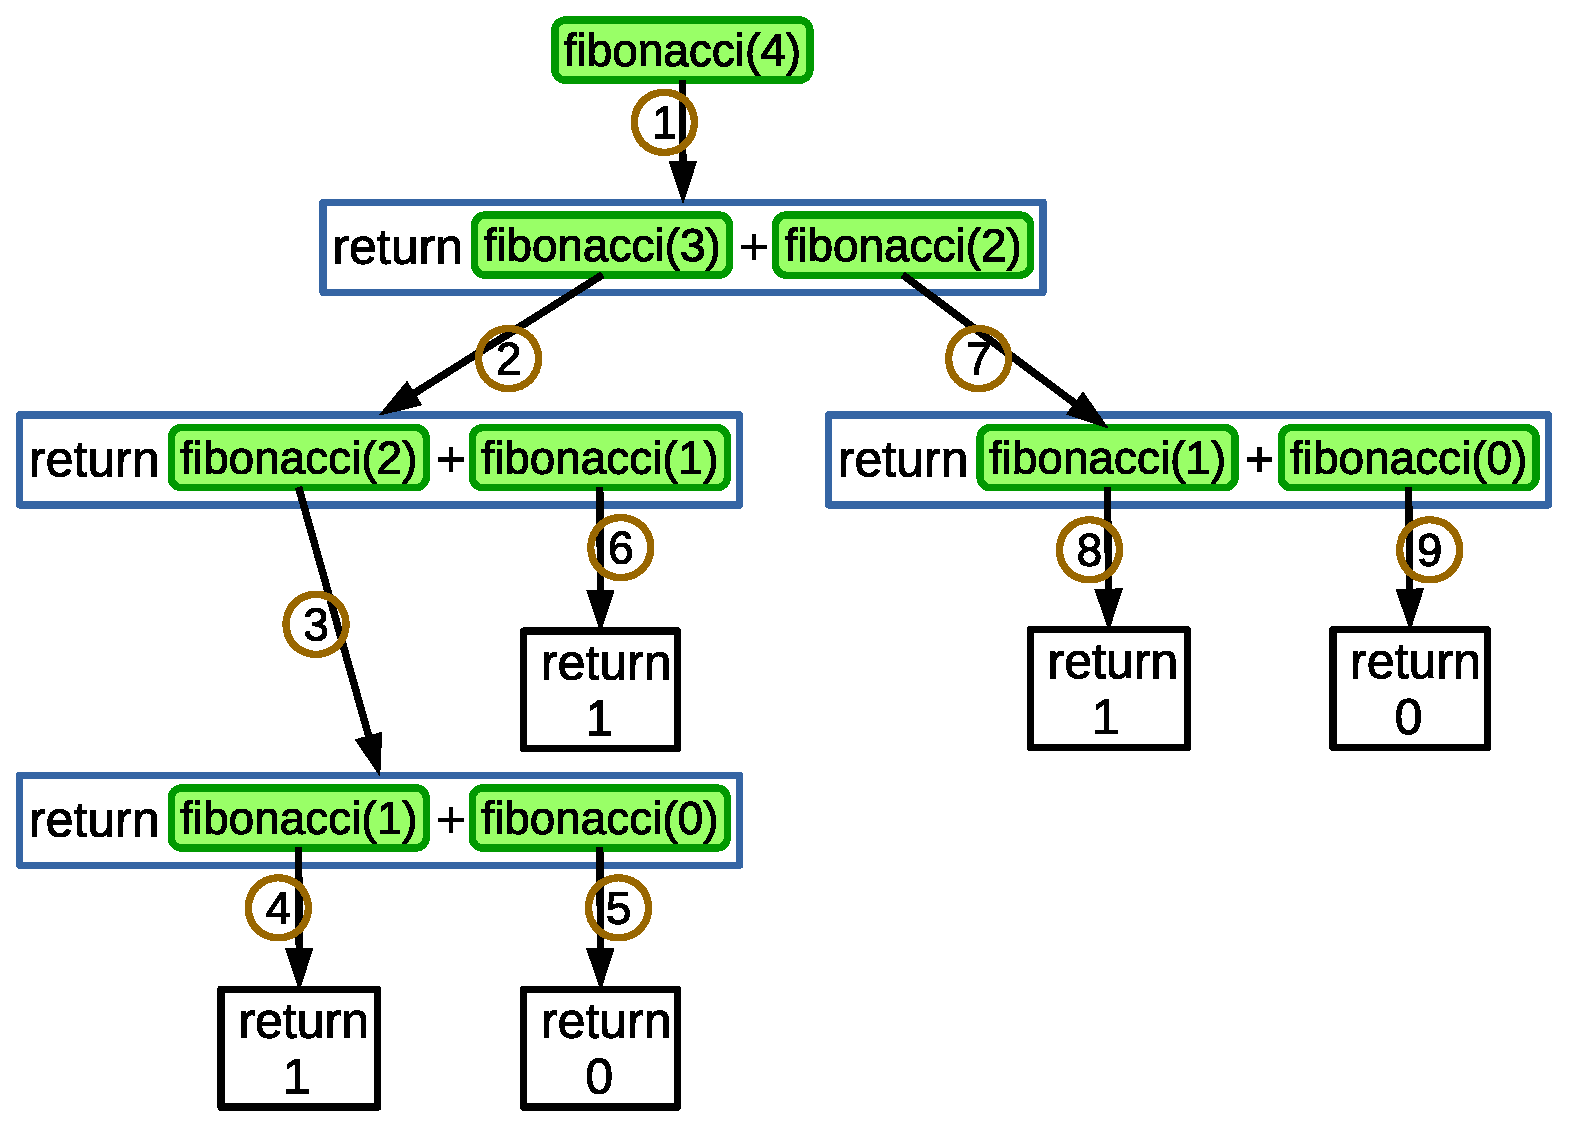
\includegraphics[height=2in]{figs2/recursion-fibonacci-depiction-0.eps}}
\afterfig

This next image depicts the value being returned by each call and the order in which those returns occur. You'll note that the initial call (where we pass in the argument 4 asking for number in the fifth position of the sequence) contains the number 3, which is the fifth number in the sequence. That is calculated based on the summing of the values from the recursive calls right below, which use the sums of values from the recursive calls below them.

\beforefig
\centerline{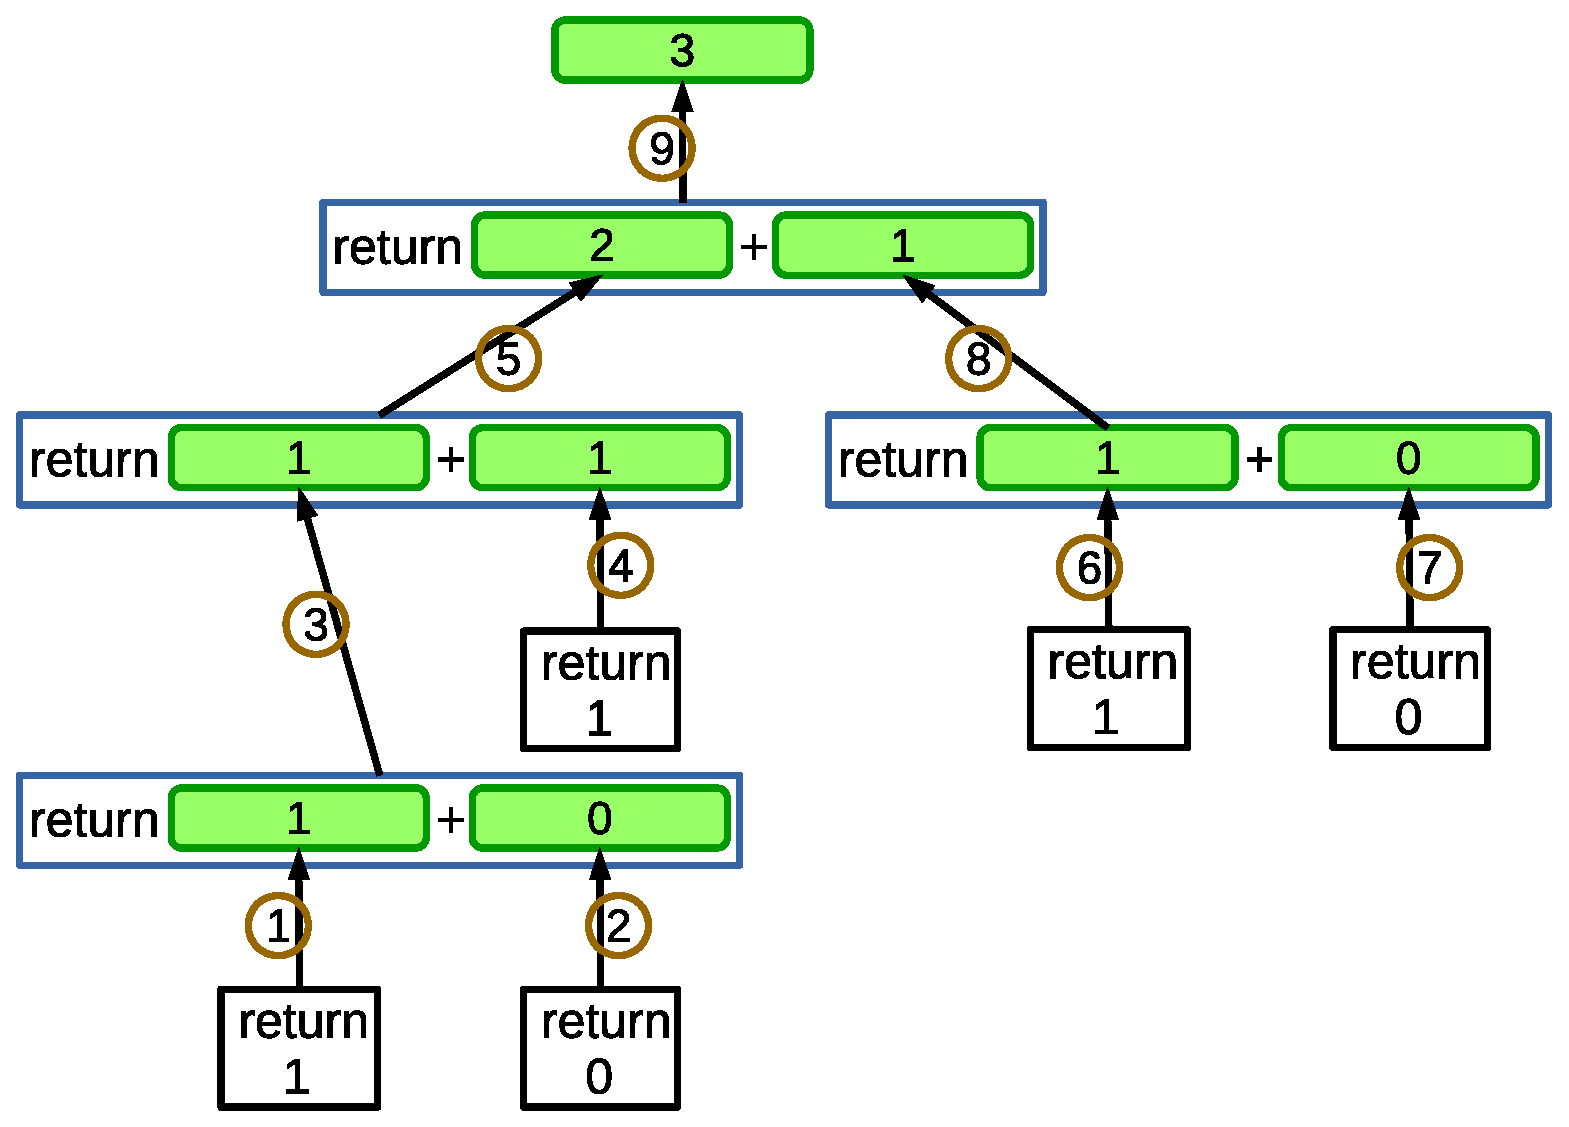
\includegraphics[height=2in]{figs2/recursion-fibonacci-depiction-1.eps}}
\afterfig

\section{Searching an ordered array}

Another example of a common recursive process is searching an ordered array for a specific value. For example, imagine we are creating a program to check the spelling of words. We already have an array of words that is stored in alphabetical order. Our program needs to accept a word from the user and tell him or her whether it is spelled correctly, or at least if it is a word that is in our array of words.

One way we could write the search would be to start at the beginning of the array and hunt through until we either find a match or arrive at the end of the array. If we find a match we can stop searching and tell the user that the word is spelled correctly. If we reach the end of the array we know the word isn't in our array and we tell the user we can't find that word.

This is a fairly inefficient approach to searching the array. If there are 1,000,000 (one million) words in the array, we will have to hunt through all million words in order to determine that a word is misspelled. If we wanted to use this to spell check a term paper, it would take a long time to run. Is there a better way?

Consider how you would do this task manually, perhaps using a dictionary. You would not start reading words at the beginning and go sequentially through until you matched the word or got to the end of the dictionary. Instead, what would you do? You would jump to the section of the dictionary that begins with the same letter that the word begins with. You would then jump several pages forward, check if the word was further on or earlier and jump forward or back in smaller and smaller increments as appropriate.

With this approach when are you done? Just like the earlier sequential approach, if you find a match you are done and you know the word is spelled correctly. What about the case where the word isn't in the dictionary? You know you are done when you find the location where the word would be if it were there. In other words, when you find two words next to each other where the first comes before the word you seek and the second comes after, you know that your word isn't present.

\section{Binary search}

To search this way using our ordered array example with a computer program we have to make one simplification to the process just described. As humans looking at a dictionary, which is generally organized to make jumping to a specific first letter easy, we can get to the correct part of the dictionary very fast. Our array, however, doesn't have a way to know where each set of words beginning with a specific letter starts. Instead we'll have the computer jump to the middle of the array and check for which of three conditions is true:

\begin{enumerate}
	\item The word in the middle of the array matches the word we are searching for
	\item The word in the middle of the array comes before (in alphabetical order) the word we are searching for
	\item The word in the middle of the array comes after the word we are searching for
\end{enumerate}

If the word is a match, we are done. We found the word and can return a result indicating the word is spelled correctly.

What about the other two cases? Based on our comparison with the word in the middle of the array we know whether the word we are searching for comes before or after the word at that location in the array.

We then logically divide the array into two parts, the set of words in the first half of the array and the set of words in the second half of the array. What we are creating are two \textbf{subarrays}, each containing half of the words that were in the original array. 

If the word we seek comes after the word we found in the middle of the original array then we know that our word, if it is present in the array at all, would have to be in the second subarray (remember the array is alphabetically ordered). In this case we do not need to look at the first subarray at all, our word can't be there.

We then treat that subarray as our array to be searched and repeat the process. We jump to the middle of that subarray and check to see which of the three conditions (listed above) are met.

In terms of set size, after our first comparison we have divided the number of words to be searched in half. After the second comparison we have reduced it to one-quarter. The third comparison reduces the amount of the array remaining to one-eighth of the original. You may notice a pattern here. With each comparison we are reducing the remaining amount of the array to search by a factor of 2 of what it was previously.

It turns out this approach of searching is amazingly efficient. In fact, to search our 1,000,000 words, the worst case number of comparisons is the square root of 1,000,000. That turns out to be 1,000. Remember though, the key to being able to do this is to have the array elements in ascending order. The name of this form of search is known as a \textbf{binary search}.

\index{binary search}

We use the term \textit{binary} for the search because it continually divides the remainder of the set in half, creating two subarrays. One subarray may hold a matching value and the other can be ignored.

How does this relate to recursion? Reviewing the process of a \textit{binary search} you'll note that it is carrying out the same operation on smaller subsets of the data. The operation always jumps to the middle of the remaining subarray, checks whether the value matches the one we seek or, if it doesn't match, figures out if the value would be earlier or later in the subarray.

The stop conditions are reached when either:

\begin{enumerate}
	\item A match is found
	\item The subdividing of the array has reduced down to a subset with one element and that element's value does not match the word we are seeking
\end{enumerate}

For this example, the information a recursive method would need includes the sorted array of words, the current start and end positions of the subarray being searched and the word being sought.

The method would check the center of the subarray for the word. If the method finds a match it is done and returns a success result, either a Boolean \texttt{true} or perhaps the array index location containing the word. 

If the word is not matched at the center of the subarray, the method will check whether the word is alphabetically greater or less than the word found in the middle of the array. It then makes a recursive call, replacing the beginning or ending value of the subarray with the location of the old center, offset by one. For example, if the word being sought is greater than the one found then the recursive call needs to check the elements from the old center plus one to the end of the subarray.

\section{Depicting a successful binary search}

Let's illustrate the process of a binary search without worrying about programming it yet. First, we'll work through a depiction of the process where the value we are searching for is in the array. 

For our example, we start with an array containing 10 fruit names in alphabetical order. In the image we see each word and to the left the element number in the array which contains that value. The array has 10 values so the array elements are numbered 0 to 9.

\beforefig
\centerline{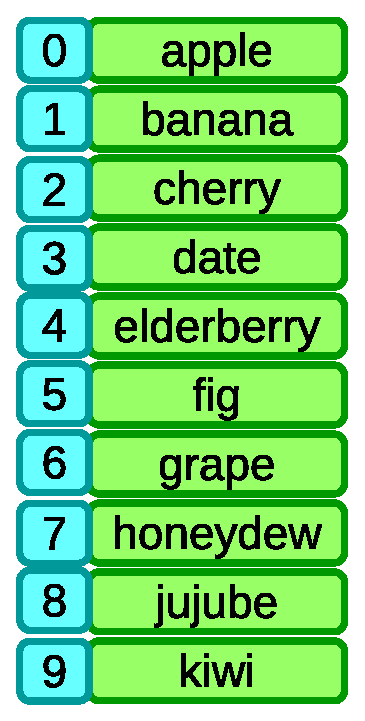
\includegraphics[height=2in]{figs2/recursion-binsearch-initiallist.eps}}
\afterfig

We want to see if the word \textbf{jujube} matches one of our words. We start by finding the middle of the array. To find the middle we add the starting index value to the ending index value and divide by 2. For this process we always use integer division (no fractional part). Given our 10 element array we calculate \texttt{(0 + 9) / 2} resulting in the integer value \texttt{4}. We compare our search term, \textbf{jujube}, to the word located in element 4, which is \textbf{elderberry}.

\beforefig
\centerline{\includegraphics[height=2in]{figs2/recursion-binsearch-success-1.eps}}
\afterfig

The words do not match, so we check to see if \textbf{jujube} comes before or after \textbf{elderberry}. It comes after, meaning that if it is in the list it must be in an element further down the array. All the elements before the one containing \textbf{elderberry}, as well as the element containing \textbf{elderberry}, cannot contain our word and do not need to be looked at.

Since we know the word would come after the position just checked, we change the starting position to be one greater than the position just checked, which is the value  5.

\beforefig
\centerline{\includegraphics[height=2in]{figs2/recursion-binsearch-success-2.eps}}
\afterfig

Now we need to repeat this process on the remaining subarray. We calculate the middle element of the remaining elements. Our updated starting element number (as described above) is 5 (one past elderberry) and the end is still 9. Our calculation is then \texttt{(5 + 9) / 2} which results in \texttt{7}. We compare our search term, \textbf{jujube}, to the word located in element 7, which is \textbf{honeydew}.

\beforefig
\centerline{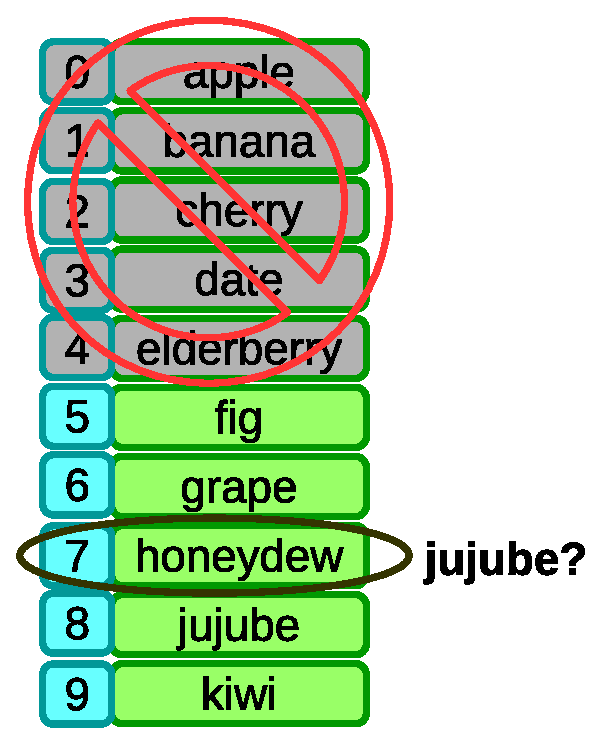
\includegraphics[height=2in]{figs2/recursion-binsearch-success-3.eps}}
\afterfig

The words do not match, so we check to see if \textbf{jujube} comes before or after \textbf{honeydew}. It comes after, meaning that if it is in the list it must be in an element further down the array. All the elements before the one containing \textbf{honeydew}, as well as the element containing \textbf{honeydew} cannot contain our word and do not need to be looked at.

Since we know the word would come after the position just checked, we again change the starting position to be one greater than the position just checked, which is the value  8.

\beforefig
\centerline{\includegraphics[height=2in]{figs2/recursion-binsearch-success-4.eps}}
\afterfig

Again we repeat this process on the remaining subarray. We calculate the middle element of the remaining elements. Our new starting element number is 8 and the end is still 9. Our calculation is then \texttt{(8 + 9) / 2} which results in \texttt{8}. We compare our search term, \textbf{jujube}, to the word located in element 8, which is \textbf{jujube}.

\beforefig
\centerline{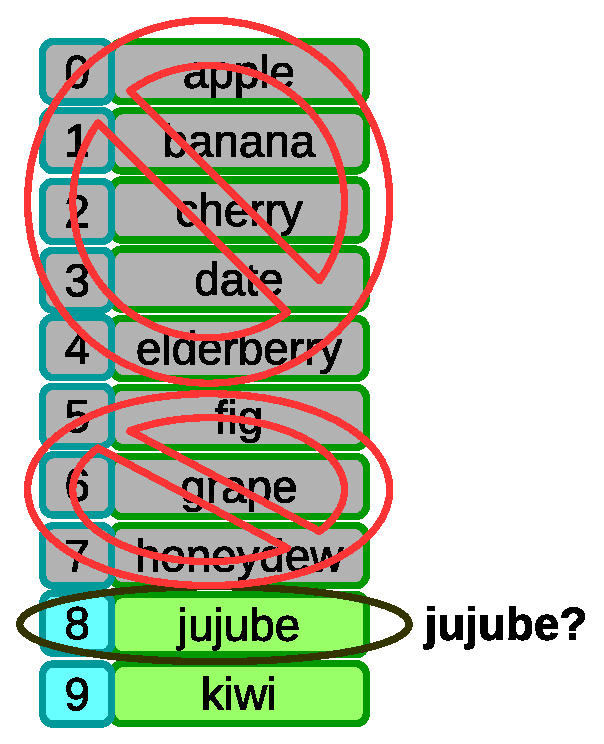
\includegraphics[height=2in]{figs2/recursion-binsearch-success-5.eps}}
\afterfig

The words match! The search is completed having made only 3 comparisons in our list of 10 elements.

\beforefig
\centerline{\includegraphics[height=2in]{figs2/recursion-binsearch-success-6.eps}}
\afterfig

\section{Depicting an unsuccessful binary search}

Here is a depiction of the binary search process where the value we are searching for is \textit{not} in the array. We start with the same array of 10 fruit names in alphabetical order. 

\beforefig
\centerline{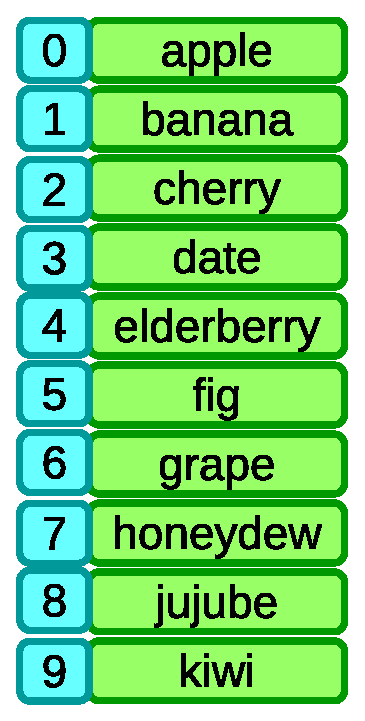
\includegraphics[height=2in]{figs2/recursion-binsearch-initiallist.eps}}
\afterfig

We want to see if the word \textbf{celery} matches one of our words. As before, we start by finding the middle of the array, element 4. We compare our search term, \textbf{celery}, to the word located in element 4, which is \textbf{elderberry}.

\beforefig
\centerline{\includegraphics[height=2in]{figs2/recursion-binsearch-failure-1.eps}}
\afterfig

The words do not match, so we check to see if \textbf{celery} comes before or after \textbf{elderberry}. It comes before, meaning that if it is in the list it must be in an element earlier in the array. All the elements after the one containing \textbf{elderberry}, as well as the element containing \textbf{elderberry}, cannot contain our word and do not need to be looked at.

Since we know the word would come before the position just checked, we change the ending position to be one less than the position just checked, which is the value 3.

\beforefig
\centerline{\includegraphics[height=2in]{figs2/recursion-binsearch-failure-2.eps}}
\afterfig

Again, we need to repeat this process on the remaining subarray. We calculate the middle element of the remaining elements. Our updated ending element number (as descrbied above) is 3 (one before elderberry) and the beginning is still 0. Our calculation is then \texttt{(0 + 3) / 2} which results in \texttt{1}. We compare our search term, \textbf{celery}, to the word located in element 1, which is \textbf{banana}.

\beforefig
\centerline{\includegraphics[height=2in]{figs2/recursion-binsearch-failure-3.eps}}
\afterfig

The words do not match, so we check to see if \textbf{celery} comes before or after \textbf{banana}. It comes after, meaning that if it is in the list it must be in an element further down the array. All the elements before the one containing \textbf{banana}, as well as the element containing \textbf{banana} cannot contain our word and do not need to be looked at.

Since we know the word would come after the position just checked, we change the starting position to be one greater than the position just checked, which is the value 2.

\beforefig
\centerline{\includegraphics[height=2in]{figs2/recursion-binsearch-failure-4.eps}}
\afterfig

As usual, we repeat the process on the remaining subarray. We calculate the middle element of the remaining elements. Our updated starting element number is 2 and the end is still 3. Our calculation is then \texttt{(2 + 3) / 2} which results in \texttt{2}. We compare our search term, \textbf{celery}, to the word located in element 2, which is \textbf{cherry}.

\beforefig
\centerline{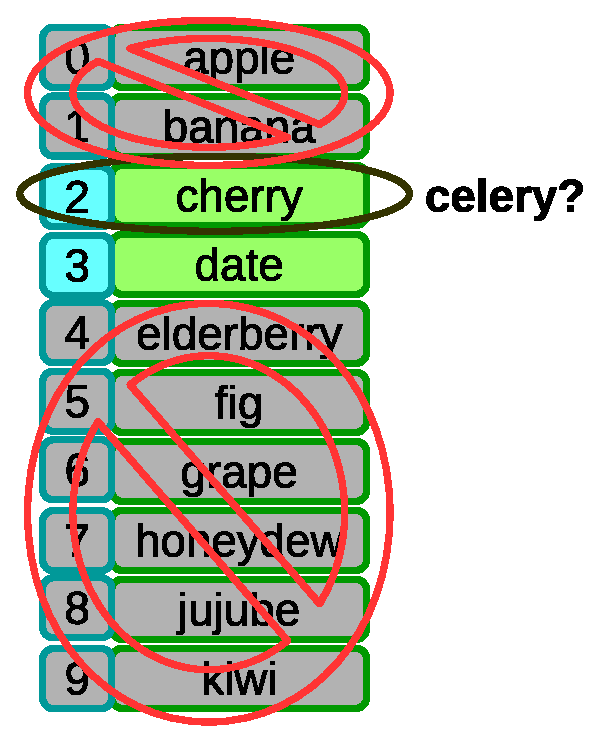
\includegraphics[height=2in]{figs2/recursion-binsearch-failure-5.eps}}
\afterfig

The words do not match, so we check to see if \textbf{celery} comes before or after \textbf{cherry}. It comes before, meaning that if it is in the list it must be in an element earlier in the array. 

Since we know the word would come before the position just checked, we change the ending position to be one less than the position just checked, which is the value 1. 

\beforefig
\centerline{\includegraphics[height=2in]{figs2/recursion-binsearch-failure-6.eps}}
\afterfig

We now find that the starting element position is 2 and the ending element position 1. Since start is greater than end we know the word can't be in the array. 

Fundamentally, \textbf{\textit{all the earlier elements and all the later elements have been ruled out}}. Therefore the word must not be in the list. We have completed the search having made only 3 comparisons in our list of 10 elements.

\section{Implementing a recursive binary search}

Let's look at the code to implement the binary search process we just described. We'll call our class \texttt{WordSearch} and create a recursive method called \texttt{binarySearch} to implement the logic.

\index{recursive method}

There are four pieces of information the method needs:

\begin{enumerate}
	\item The ordered array of words
	\item The word we are searching for
	\item The current starting array element number
	\item The current ending array element number
\end{enumerate}

In the binary search process we will first calculate the center element. We will also need a variable to house the result of comparing the word being sought to the word in the center element of the subarray.

Next we need to compare the words (strings). Java has a string comparison method \texttt{compareToIgnoreCase()} which is perfect for our purposes. It will return 0 (zero) if the words match, a negative number if the word comes before the word being compared and a positive number if the word comes after the word being compared.

\index{compareToIgnoreCase}

For example, the Java code:

\beforeverb
\begin{verbatim}
int comparison = "Grape".compareToIgnoreCase("Apple");
System.out.println(comparison);
\end{verbatim}
\afterverb

Would output the value:

\beforeverb
\begin{verbatim}
6
\end{verbatim}
\afterverb

This means that the word \textit{Grape} comes after (alphabetically) the word \textit{Apple}. We don't need to be concerned with the specific value of 6. All that matters to us in this case is that if the number is greater than 0, the word comes after the word being compared and if it is negative the word comes before the word being compared.\footnote{If you are curious, the value returned is the lexical distance between the first unique letters encountered in the words. In this case the letter 'G' is 6 letters greater than the letter 'A'.}

The next part of the method will need to evaluate the result of the comparison, which we'll store in a variable called \texttt{comparison}. 

\begin{enumerate}
	\item If the value is 0 then we have found a match and we'll return the array index position of the element containing the word. 
	\item If the value is less than 0 we will update the ending array element number to be one less than the current center position (e.g. we know the word has to be earlier in the array).
	\item If the value is greater than 0 we will update the starting array element number to be one more than the current center position (e.g. we know the word has to be later in the array).
\end{enumerate}

Finally we need to determine whether we have reached the end of the process, meaning there is no smaller subset of the original array left to search. The easiest way to figure that out is to compare the updated start and end positions. If they cross, meaning that the start position becomes greater than the end position, we have finished the search and not found a match. If the start position is equal to or less than the end position we need to recurse and check the new subarray.

Here is the entire method, which implements the process just described. Make sure that each part makes sense and that you can see how the code relates to the explanation above.

\beforeverb
\begin{verbatim}
public class WordSearchNoTracing {
 private int binarySearch(String[] wordList, String searchTerm,
                                      int startPos, int endPos) {
  int checkPosition = (startPos + endPos) / 2;
  int comparison;

  // Compare the search term to the word in the center element of the
  // subarray
  comparison = searchTerm.compareToIgnoreCase(wordList[checkPosition]);

  if (comparison == 0) {
   // The words matched - return the matching position in the array
   return checkPosition;
  } else if (comparison < 0) {
   // The search term comes earlier in the array, change the ending
   // position
   endPos = checkPosition - 1;
  } else {
   // The search term comes later in the array, change the beginning
   // position
   startPos = checkPosition + 1;
  }

  // Check that there are still words left to check
  if (startPos <= endPos) {
   // Make a recursive call to search the new subarray
   return binarySearch(wordList, searchTerm, startPos, endPos);
  } else {
   // If the set was reduced to a single element with no match then the
   // word is not present
   return -1;
  }
 }

 public static void main(String[] args) {
  String[] fruits = { "apple", "banana", "cherry", "date", "elderberry", "fig",
      "grape", "honeydew", "jujube", "kiwi" };
  WordSearchNoTracing instance = new WordSearchNoTracing();

  int foundPosition = instance.binarySearch(fruits, "jujube", 0, fruits.length - 1);
  System.out.println("Find jujube? " + foundPosition);

  System.out.println("=============================");
  
  foundPosition = instance.binarySearch(fruits, "carrot", 0, fruits.length - 1);
  System.out.println("Find carrot? " + foundPosition);
 }
}
\end{verbatim}
\afterverb

When we run this we see the following output:

\beforeverb
\begin{verbatim}
Find jujube? 8
=============================
Find carrot? -1
\end{verbatim}
\afterverb

This means that \textit{jujube} was found in element 8 of the \texttt{fruits} array and \textit{carrot} was not found in the array (we chose to use -1 as the signal for not finding a match).

Let's add a few print statements so that we can see what is happening when the \texttt{binarySearch} method runs. Here is an updated version that includes some \texttt{System.out.println} calls to display the internal values as the recursive calls are made. 


\beforeverb
\begin{verbatim}
public class WordSearch {
 private int binarySearch(String[] wordList, String searchTerm, 
                                      int startPos, int endPos) {
  int checkPosition = (startPos + endPos) / 2;
  int comparison;

  System.out.println(
    "BinarySearch called for searchTerm:" + searchTerm + " 
               startPos:" + startPos + " endPos:" + endPos);

  // Compare the search term to the word in the center element of the
  // subarray
  comparison = searchTerm.compareToIgnoreCase(wordList[checkPosition]);

  System.out.println("checkPosition:" + checkPosition +
       " WordAtPosition:" + wordList[checkPosition] + 
       " comparison:" + comparison);

  if (comparison == 0) {
   // The words matched - return the matching position in the array
   System.out.println("Words matched at checkPosition: " + checkPosition);
   System.out.println();
   return checkPosition;
  } else if (comparison < 0) {
   // The search term comes earlier in the array, change the ending
   // position
   endPos = checkPosition - 1;
  } else {
   // The search term comes later in the array, change the beginning
   // position
   startPos = checkPosition + 1;
  }

  // Check that there are still words left to check
  if (startPos <= endPos) {
   // Make a recursive call to search the new subarray
   System.out.println("Make a recursive call. startPos:" + 
                             startPos + " endPos:" + endPos);
   System.out.println();
   return binarySearch(wordList, searchTerm, startPos, endPos);
  } else {
   // If the set was reduced to a single element with no match then the
   // word is not present
   System.out.println("No more elements to be searched. startPos:" + 
                                       startPos + " endPos:" + endPos);
   System.out.println();
   return -1;
  }
 }

 public static void main(String[] args) {
  String[] fruits = { "apple", "banana", "cherry", "date", "elderberry", "fig",
      "grape", "honeydew", "jujube", "kiwi" };
  WordSearch instance = new WordSearch();

  int foundPosition = instance.binarySearch(fruits, "jujube", 0, fruits.length - 1);
  System.out.println("Find jujube? " + foundPosition);

  System.out.println("=============================");

  foundPosition = instance.binarySearch(fruits, "carrot", 0, fruits.length - 1);
  System.out.println("Find carrot? " + foundPosition);
 }
}
\end{verbatim}
\afterverb

When we run this we see some details about how the recursive calls are operating:

\beforeverb
\begin{verbatim}
BinarySearch called for searchTerm:jujube startPos:0 endPos:9
checkPosition:4 WordAtPosition:elderberry comparison:5
Make a recursive call. startPos:5 endPos:9

BinarySearch called for searchTerm:jujube startPos:5 endPos:9
checkPosition:7 WordAtPosition:honeydew comparison:2
Make a recursive call. startPos:8 endPos:9

BinarySearch called for searchTerm:jujube startPos:8 endPos:9
checkPosition:8 WordAtPosition:jujube comparison:0
Words matched at checkPosition: 8

Find jujube? 8
=============================
BinarySearch called for searchTerm:carrot startPos:0 endPos:9
checkPosition:4 WordAtPosition:elderberry comparison:-2
Make a recursive call. startPos:0 endPos:3

BinarySearch called for searchTerm:carrot startPos:0 endPos:3
checkPosition:1 WordAtPosition:banana comparison:1
Make a recursive call. startPos:2 endPos:3

BinarySearch called for searchTerm:carrot startPos:2 endPos:3
checkPosition:2 WordAtPosition:cherry comparison:-7
No more elements to be searched. startPos:2 endPos:1

Find carrot? -1
\end{verbatim}
\afterverb

Make sure to study the output and trace through the recursive method calls that are executed in these examples. Drawing a table of values and keeping track of the \textit{stack} of parameter and local variable values may be helpful as well.


\iffalse

\section{Tower of Hanoi}

A classic mathematical puzzle which requires this type of problem solving is known as the \textbf{Tower of Hanoi}.\footnote{https://en.wikipedia.org/wiki/Tower\textunderscore of\textunderscore Hanoi}

The puzzle is comprised of a base with three vertical posts and a set of disks with different diameters. The disks have a hole in the center so that they may be stacked on the vertical posts. The initial setup requires the player to stack, in order from largest (on the bottom) to smallest (on the top), all of the disks on one of the posts. 

The objective of the game is to move the disks and recreate the ordered stack on a different post. The rules are simple:

\begin{enumerate}
	\item Only one disk may be moved at a time
	\item A move consists of picking up one disk and moving it to another post. The disk must be the top most disk on one of the posts
	\item A larger diameter disk may never be placed on a smaller diameter disk
\end{enumerate}

It turns out that an effective strategy for solving this puzzle is to break the problem down into smaller steps. Instead of worrying about all the disks we can concentrate on the first two. We can move them onto the two empty posts. We can then move the smaller of the two on top of the larger of the two. We can then move the third disks to the empty post, put the smallest disk back on the original post and the second-smallest disk on the  
subset 

\fi

\section{Glossary}

\begin{description}

\item[recurse:] Having a method call itself, typically with a subset of the data that was provided to the initial method call. 
\index{recurse}

\item[recursion:] The use of a method that uses its own definition to apply the same logic over and over. Typically this is used to break a large problem into smaller pieces and ultimately solve the larger problem by combining the results of the recursive calls.
\index{recursion}

\item[recursive method:] A method that uses recursion.
\index{recursive method}

\item[stack:] A data structure where information (data) is placed in an ordered list. In the case of recursion, the stack holds the data from earlier calls to a recursive method that are waiting on results from their recursive calls. As recursive calls end, the previous data is retrieved from the stack and restored for the earlier method call to use.
\index{stack}

\end{description}

\newpage

\section{Exercises}

\begin{ex}
Write a program that takes an ordered array of integers and uses a binary search to find a specific number. Assume the numbers are all positive allowing you to use -1 as the signal for not finding a match. You should be able to use the example WordSearch class from the chapter as a starting point for this program.
\end{ex}

\begin{ex}
Write a program that prompts the user for a positive number and then sums all the numbers from 1 up to the entered value. The program \textbf{may \textit{not} use a loop}. Rather, it must use a recursive method to carry out the summing process.
Here is an example of what a run of the program would look like:

\beforeverb
\begin{verbatim}
Enter a positive number: 5
Result: 15
\end{verbatim}
\afterverb

\end{ex}


\begin{ex}
Sometimes when programmers get bored or want to have a bit of fun,
they add a harmless {\bf Easter Egg}\footnote{\url{en.wikipedia.org/wiki/Easter_egg_(media)}} to their program. Modify the program from the previous exercise so that it prints a funny
message when the user types a specific value. For example you might have the program print the message \texttt{ Answer to the Ultimate Question of Life, the Universe, and Everything} when the user enters the number 42. 
The program should behave normally for all other supplied values.  Here are a couple of sample executions of the program:

\beforeverb
\begin{verbatim}
Enter a positive number: 42
Answer to the Ultimate Question of Life, the Universe, and Everything
Result: 903

Enter a positive number: 7
Result: 28
\end{verbatim}
\afterverb
%
We are not encouraging you to put Easter Eggs in your 
programs---this is just an exercise.

\end{ex}


% LaTeX source for ``Introduction to Computer Science (Python Edition)''
% Copyright (c) 2021- David S. Read, All Rights Reserved
% Built upon, ``Python for Informatics: Exploring Information''
% Copyright (c)  2010-  Charles R. Severance, All Rights Reserved

\chapter{Strings}
\label{strings}


\section{A string is a sequence}
\index{sequence}
\index{character}
\index{bracket operator}
\index{operator!bracket}

A string is a {\bf sequence} of characters.  
You can access the characters one at a time with the
bracket operator:

\beforeverb
\begin{verbatim}
>>> fruit = 'banana'
>>> letter = fruit[1]
\end{verbatim}
\afterverb
%
\index{index}
The second statement extracts the character at index position 1 from the 
{\tt fruit} variable and assigns it to the {\tt letter} variable.  

The expression in brackets is called an {\bf index}.  
The index indicates which character in the sequence you
want (hence the name).

But you might not get what you expect:

\beforeverb
\begin{verbatim}
>>> print(letter)
a
\end{verbatim}
\afterverb
%
For most people, the first letter of \verb"'banana'" is {\tt b}, not
{\tt a}.  But in Python, the index is an offset from the
beginning of the string, and the {\bf offset of the first letter is zero}.

\beforeverb
\begin{verbatim}
>>> letter = fruit[0]
>>> print(letter)
b
\end{verbatim}
\afterverb
%
So {\tt b} is the 0th letter (``zero-eth'') of \verb"'banana'", {\tt a}
is the 1th letter (``one-eth''), and {\tt n} is the 2th (``two-eth'')
letter.

\beforefig
\centerline{\includegraphics[height=0.50in]{figs2/string.eps}}
\afterfig

\index{index!starting at zero}
\index{zero, index starting at}

You can use any expression, including variables and operators, as an
index, but the value of the index has to be an integer.  Otherwise you
get:

\index{index}
\index{exception!TypeError}
\index{TypeError}

\beforeverb
\begin{verbatim}
>>> letter = fruit[1.5]
TypeError: string indices must be integers
\end{verbatim}
\afterverb
%

\section{Getting the length of a string using {\tt len}}

\index{len function}
\index{function!len}

{\tt len} is a built-in function that returns the number of characters
in a string:

\beforeverb
\begin{verbatim}
>>> fruit = 'banana'
>>> len(fruit)
6
\end{verbatim}
\afterverb
%
To get the last letter of a string, you might be tempted to try something
like this:

\index{exception!IndexError}
\index{IndexError}

\beforeverb
\begin{verbatim}
>>> length = len(fruit)
>>> last = fruit[length]
IndexError: string index out of range
\end{verbatim}
\afterverb
%
The reason for the {\tt IndexError} is that there is no letter in {\tt
'banana'} with the index 6.  Since we started counting at zero, the
six letters are numbered 0 to 5.  To get the last character, you have
to subtract 1 from {\tt length}:

\beforeverb
\begin{verbatim}
>>> last = fruit[length-1]
>>> print(last)
a
\end{verbatim}
\afterverb
%
Alternatively, you can use negative indices, which count backward from
the end of the string.  The expression {\tt fruit[-1]} yields the last
letter, {\tt fruit[-2]} yields the second to last, and so on.

\index{index!negative}
\index{negative index}


\section{Traversal through a string with a loop}
\label{for}

\index{traversal}
\index{loop!traversal}
\index{for loop}
\index{loop!for}
\index{statement!for}
\index{traversal}
\index{while loop}
\index{loop!while}
\index{statement!while}

A lot of computations involve processing a string one character at a
time.  Often they start at the beginning, select each character in
turn, do something to it, and continue until the end.  This pattern of
processing is called a {\bf traversal}.  

\label{ch6StringTraversal}
One way to write a traversal
is with a {\tt while} loop:

\beforeverb
\begin{verbatim}
index = 0
while index < len(fruit):
    letter = fruit[index]
    print(letter)
    index = index + 1
\end{verbatim}
\afterverb
%
This loop traverses the string and displays each letter on a line by
itself.  The loop condition is {\tt index < len(fruit)}, so
when {\tt index} is equal to the length of the string, the
condition is false, and the body of the loop is not executed.  The
last character accessed is the one with the index {\tt len(fruit)-1},
which is the last character in the string.

Another way to write a traversal is with a {\tt for} loop:

\beforeverb
\begin{verbatim}
for char in fruit:
    print(char)
\end{verbatim}
\afterverb
%
Each time through the loop, the next character in the string is assigned
to the variable {\tt char}.  The loop continues until no characters are
left.


\section{String slices}
\label{slice}

\index{slice operator}
\index{operator!slice}
\index{index!slice}
\index{string!slice}
\index{slice!string}

A segment of a string is called a {\bf slice} or {\bf substring}.  Selecting a slice is
similar to selecting a character:

\beforeverb
\begin{verbatim}
>>> s = 'Monty Python'
>>> print(s[0:5])
Monty
>>> print(s[6:12])
Python
\end{verbatim}
\afterverb
%
The operator {\tt [n:m]} returns the part of the string from the 
``n-eth'' character to the ``m-eth'' character, including the first {\bf but
excluding the last}.  

If you omit the first index (before the colon), the slice starts at
the beginning of the string.  If you omit the second index, the slice
goes to the end of the string:

\beforeverb
\begin{verbatim}
>>> fruit = 'banana'
>>> fruit[:3]
'ban'
>>> fruit[3:]
'ana'
\end{verbatim}
\afterverb
%
If the first index is greater than or equal to the second the result
is an {\bf empty string}, represented by two quotation marks:

\index{quotation mark}

\beforeverb
\begin{verbatim}
>>> fruit = 'banana'
>>> fruit[3:3]
''
\end{verbatim}
\afterverb
%
An empty string contains no characters and has length 0, but other
than that, it is the same as any other string.


\index{copy!slice}
\index{slice!copy}

When you take a slice from a string, the slice is a new string. It contains a copy of the characters from the range of the slice.

The slice (or substring) convention of including the first index character and excluding the last is common when working with strings in many languages. There are two advantages to this approach. First, you may use the length of the string as the second value in the slice to get the last character in the string. Second, if you subtract the starting index from the ending index the result is the number of characters placed in the slice.

\section{Strings are immutable}
\index{mutability}
\index{immutability}
\index{string!immutable}

It is tempting to use the {\tt []} operator on the left side of an
assignment, with the intention of changing a character in a string.
For example:

\index{TypeError}
\index{exception!TypeError}

\beforeverb
\begin{verbatim}
>>> greeting = 'Hello, world!'
>>> greeting[0] = 'J'
TypeError: object does not support item assignment
\end{verbatim}
\afterverb
%
The ``object'' in this case is the string and the ``item'' is
the character you tried to assign.  For now, an {\bf object} is
the same thing as a value, but we will refine that definition
later.  An {\bf item} is one of the values in a sequence.

\index{object}
\index{item assignment}
\index{assignment!item}
\index{immutability}
\index{concatenate}

The reason for the error is that
strings are {\bf immutable}, which means you can't change an
existing string.  The best you can do is create a new string
that is a variation on the original:

\beforeverb
\begin{verbatim}
>>> greeting = 'Hello, world!'
>>> new_greeting = 'J' + greeting[1:]
>>> print(new_greeting)
Jello, world!
\end{verbatim}
\afterverb
%
This example concatenates a new first letter onto
a slice of {\tt greeting}.  It has no effect on
the original string.

\index{concatenation}

\section{Looping and counting}
\label{counter}

\index{counter}
\index{counting and looping}
\index{looping and counting}
\index{looping!with strings}

\label{ch6LetterCount}
The following program counts the number of times the letter {\tt a}
appears in a string:

\beforeverb
\begin{verbatim}
word = 'banana'
count = 0
for letter in word:
    if letter == 'a':
        count = count + 1
print(count)
\end{verbatim}
\afterverb
%
This program demonstrates another pattern of computation called a {\bf
counter}.  The variable {\tt count} is initialized to 0 and then
incremented each time an {\tt a} is found.
When the loop exits, {\tt count}
contains the result---the total number of {\tt a}'s.

\section{The {\tt in} operator}
\label{inboth}

\index{in operator}
\index{operator!in}
\index{boolean operator}
\index{operator!boolean}

The word {\tt in} is a boolean operator that takes two strings and
returns {\tt True} if the first appears as a substring in the second:

\beforeverb
\begin{verbatim}
>>> 'a' in 'banana'
True
>>> 'seed' in 'banana'
False
\end{verbatim}
\afterverb
%

\section{String comparison}

\index{string!comparison}
\index{comparison!string}

The comparison operators work on strings.  To see if two strings are equal:

\beforeverb
\begin{verbatim}
if word == 'banana':
    print('All right, bananas.')
\end{verbatim}
\afterverb
%
Other comparison operations are useful for putting words in alphabetical
order:

\beforeverb
\begin{verbatim}
if word < 'banana':
    print('Your word,' + word + ', comes before banana.')
elif word > 'banana':
    print('Your word,' + word + ', comes after banana.')
else:
    print('All right, bananas.')
\end{verbatim}
\afterverb
%
Python does not handle uppercase and lowercase letters the same way
that people do.  All the uppercase letters come before all the
lowercase letters, so:

\beforeverb
\begin{verbatim}
Your word, Pineapple, comes before banana.
\end{verbatim}
\afterverb
%
A common way to address this problem is to convert strings to a
standard format, such as all lowercase, before performing the
comparison.  Keep that in mind in case you have to defend yourself
against a man armed with a Pineapple.

To understand how we could convert a string to lowercase characters we need to delve into accessing a string's methods.

\section{{\tt string} methods}

Strings are an example of Python {\bf objects}.  An object is also known as an {\bf instance}. Each object contains
data (in this case the actual string itself) and has access to {\bf methods}, which
are effectively functions that are built for each instance to use. The data and methods are defined by the type\footnote{We will spend a great deal of time later in the semester creating our own types and objects}.

We can list the methods available to an object (instance) using Python's {\tt dir} function, which lists the methods available
for an object.  We've already seen that the {\tt type} function shows the type of an object. We can use the {\tt help} function to read documentation for a method, if the programmer of the method included such documentation.

\beforeverb
\begin{verbatim}
>>> stuff = 'Hello world'
>>> type(stuff)
<type 'str'>
>>> dir(stuff)
['capitalize', 'center', 'count', 'decode', 'encode', 
'endswith', 'expandtabs', 'find', 'format', 'index', 
'isalnum', 'isalpha', 'isdigit', 'islower', 'isspace', 
'istitle', 'isupper', 'join', 'ljust', 'lower', 'lstrip', 
'partition', 'replace', 'rfind', 'rindex', 'rjust', 
'rpartition', 'rsplit', 'rstrip', 'split', 'splitlines', 
'startswith', 'strip', 'swapcase', 'title', 'translate', 
'upper', 'zfill']
>>> help(str.capitalize)
Help on method_descriptor:

capitalize(...)
    S.capitalize() -> string
    
    Return a copy of the string S with only its first character
    capitalized.
>>>
\end{verbatim}
\afterverb
%

While the {\tt dir} function lists the methods, and you 
can use {\tt help} to get some simple documentation on a method, 
a better source of documentation for string methods would be
\url{https://docs.python.org/3/library/stdtypes.html#string-methods}.

Calling a {\bf method} is similar to calling a function---it 
takes arguments and returns a value---but the syntax is different.
We call a method by appending the method name to the variable name
using the period as a delimiter.

For example, the
method {\tt upper} returns a new string with
all uppercase letters using the string it is run on as the original value:

\index{method}
\index{string!method}

Instead of the function syntax {\tt upper(word)}, it uses
the method syntax {\tt word.upper()}.

\index{dot notation}

\beforeverb
\begin{verbatim}
>>> word = 'banana'
>>> new_word = word.upper()
>>> print(new_word)
BANANA
\end{verbatim}
\afterverb
%
This form of dot notation specifies the name of the method, {\tt
upper}, and the name of the string to apply the method to, {\tt
word}.  The empty parentheses indicate that this method takes no
argument.

\index{parentheses!empty}

A method call is called an {\bf invocation}; in this case, we would
say that we are invoking {\tt upper} on the {\tt word} object (instance).

\index{invocation}

For example, there is a string method named {\tt find} that
searches for the position of one string within another:

\beforeverb
\begin{verbatim}
>>> word = 'banana'
>>> index = word.find('a')
>>> print(index)
1
\end{verbatim}
\afterverb
%
In this example, we invoke {\tt find} on {\tt word} and pass
the letter we are looking for as a parameter.

The {\tt find} method can find substrings as well as characters:

\beforeverb
\begin{verbatim}
>>> word.find('na')
2
\end{verbatim}
\afterverb
%
It can take as a second argument the index where it should start:

\index{optional argument}
\index{argument!optional}

\beforeverb
\begin{verbatim}
>>> word.find('na', 3)
4
\end{verbatim}
\afterverb
%
One common task is to remove white space (spaces, tabs, or newlines) from
the beginning and end of a string using the {\tt strip} method:

\beforeverb
\begin{verbatim}
>>> line = '  Here we go  '
>>> line.strip()
'Here we go'
\end{verbatim}
\afterverb
%
Some methods such as {\bf startswith} return boolean values.

\beforeverb
\begin{verbatim}
>>> line = 'Please have a nice day'
>>> line.startswith('Please')
True
>>> line.startswith('p')
False
\end{verbatim}
\afterverb
%
\label{ch6StartsWithExample}
You will note that {\tt startswith} requires case to match, so sometimes
we take a line and map it all to lowercase before we do any checking
using the {\tt lower} method.

\beforeverb
\begin{verbatim}
>>> line = 'Please have a nice day'
>>> line.startswith('p')
False
>>> line.lower()
'please have a nice day'
>>> line.lower().startswith('p')
True
\end{verbatim}
\afterverb
%
In the last example, the method {\tt lower} is called
and then we use {\tt startswith}
to see if the resulting lowercase string
starts with the letter ``p''.  As long as we are careful
with the order, we can make multiple method calls in a
single expression.

\section{Parsing strings}

Often, we want to look into a string and find a substring.  For example
if we were presented a series of lines formatted as follows:

\beforeverb
\begin{alltt}
From stephen.marquard@{\bf uct.ac.za} Sat Jan  5 09:14:16 2008
\end{alltt}
\afterverb

and we wanted to pull out only the second half of the address (i.e.,
{\tt uct.ac.za}) from each line, we can do this by using the {\tt find}
method and string slicing.   

First, we will find the position of the at-sign (@) in the string.  Then we will
find the position of the first space \emph{after} the at-sign.  And then we
will use string slicing to extract the portion of the string which we 
are looking for.

\beforeverb
\begin{verbatim}
>>> data = 'From stephen.marquard@uct.ac.za Sat Jan  5 09:14:16 2008'
>>> atpos = data.find('@')
>>> print(atpos)
21
>>> sppos = data.find(' ',atpos)
>>> print(sppos)
31
>>> host = data[atpos+1:sppos]
>>> print(host)
uct.ac.za
>>> 
\end{verbatim}
\afterverb
%
We use a version of the {\tt find} method which allows us to specify
a position in the string where we want {\tt find} to start looking.
When we slice, we extract the characters 
from ``one beyond the at-sign through up to \emph{but not including} the 
space character''.  

The documentation for the {\tt find} method is available at
\url{https://docs.python.org/3/library/stdtypes.html#string-methods}.

\section{Format strings}	

\index{format strings}
\index{strings!format}

A {\bf format string} contains text and {\bf replacement fields}, which are delineated with curly braces, \{\}. Format strings allow us to create strings that combine text with other values, including literals and variables.

As an example, if we were writing a game and wanted to display the current score we might display the message:
\beforeverb
\begin{verbatim}
Current score is 5
\end{verbatim}
\afterverb

However, the score value, 5 as shown above, can't be part of the hardcoded string's text. Instead it is probably being stored in a variable, since it can change as the user plays the game. The current score needs to be included in the string where the 5 is shown.

That's where a format string becomes useful, allowing us to combine text with replacement fields. Here is a format string that could be used for the score example. It starts with the text {\tt Current score is} and then includes a replacement field to specify that some value should be inserted at that point in the string:

\beforeverb
\begin{verbatim}
'Current score is {}'
\end{verbatim}
\afterverb


Later, we'll see that we can include values in the replacement field to control the formatting of data. If the braces are left empty, {\tt \{\}}, the default representation for the data will be used. In all cases, the result is a string.

We call the {\tt format} method to provide the values used in place of the replacement fields in the format string. Let's put the score example together:

\beforeverb
\begin{verbatim}
>>> score = 6
>>> message = 'Current score is {}'.format(score)
>>> print(message)
Current score is 6
\end{verbatim}
\afterverb

The {\tt message} variable is assigned a value using a format string. The resulting value is \verb"'Current score is 6'", where the {\tt 6} is the {\tt score} variable's value being passed to the {\tt format} method. If you think about all the programs that you use and all the ways they show you information, mixing data with text, this technique becomes very handy.

We can place more than one replacement field in a string. Here is a basic example which uses two variables' values as part of the string being printed:

\beforeverb
\begin{verbatim}
>>> camels = 42
>>> elk = 25
>>> message = 'There are {} camels and {} elk.'.format(camels, elk)
>>> print(message)
There are 42 camels and 25 elk.
\end{verbatim}
\afterverb
%
Again, the {\tt message} variable is assigned a value using a format string. The resulting value is \verb"'There are 42 camels and 25 elk.'", where {\tt 42} and {\tt 25} are values taken from the variables passed to the {\tt format} method.

Replacement fields may appear anywhere in a format string,
so you can embed values anywhere in a sentence. Here is an example using three replacement fields, one at the begining, one near the middle, and one at the very end:

\beforeverb
\begin{verbatim}
>>> label_id = 1
>>> camels = 42
>>> mood = 'happy'
>>> print('{}: The {} camels are {}'.format(label_id, camels, mood))
1: The 42 camels are happy
\end{verbatim}
\afterverb
%

Values passed to the {\tt format} method may be any sort of data, such as integers, floats, and strings. By default, for each replacement field in the string, there must be a variable passed to {\tt format}. The values are used in left to right order.

You can control the formatting of data as it is included in the string. For instance, you can limit the number of decimal places displayed for a number or set the value to be left or right justified. Formatting is controlled by adding {\bf format specifications} within the curly braces of the replacement field.

Let's demonstrate some formatting capabilities. We'll begin by formatting numeric values, limiting the width of a value and the number of decimal places displayed.

To set the desired width (number of characters occupied by the number) and the number of decimal places, we define a format specification starting with a colon, followed by the total number of characters to display (width), a dot, the number of digits after the decimal point to display, and the letter {\bf f}, indicating a floating point value.

Our next examples will set the number of decimal places without limiting the width (we'll place no number before the dot in the format specification of the replacement field). Look carefully at the output and be sure you understand what is happening.

\beforeverb
\begin{verbatim}
>>> print('{:.0f}'.format(3000.14159))
3000
>>> print('{:.1f}'.format(3000.14159))
3000.1
>>> print('{:.2f}'.format(3000.14159))
3000.14
>>> print('{:.5f}'.format(3000.14159))
3000.14159
>>> print('{:.10f}'.format(3000.14159))
3000.1415900000
>>>
\end{verbatim}
\afterverb
%
 
Now let's try setting the width as well. \emph{Note that the width is a minimum.} If the whole number portion of a value is too large for the width, it will not be truncated. Instead, the width will be increased to include all the digits to the left of the decimal point. 


\beforeverb
\begin{verbatim}
>>> print('{:1.0f}'.format(3000.14159))
3000
>>> print('{:4.0f}'.format(3000.14159))
3000
>>> print('{:10.0f}'.format(3000.14159))
      3000
>>> print('{:10.2f}'.format(3000.14159))
   3000.14
\end{verbatim}
\afterverb
%

{\bf Why do the last two examples start with empty spaces?} Hint: the third printed value contains 6 spaces before the 3000 and the fourth printed value contains 3 spaces before the 3000.14

You can format string values in a similar way, controlling the width and also the text justification (left, right, and centered). The characters \textbf{$>$}, \textbf{$<$}, and \textbf{\^} are used to control right, left, and center justification, respectively. Justification works with numeric values as well. As with numbers, the width given in the replacement field is the minimum number of characters Python will use. If the string is longer, then the width will grow to accomodate.

\newpage

\beforeverb
\begin{verbatim}
>>> print('{:2}'.format('Hi!'))
Hi!
>>> print('{:3}'.format('Hi!'))
Hi!
>>> print('{:20}'.format('Hi!'))
Hi!                 
>>> print('{:<20}'.format('Hi!'))
Hi!                 
>>> print('{:>20}'.format('Hi!'))
                 Hi!
>>> print('{:^20}'.format('Hi!'))
        Hi!         
\end{verbatim}
\afterverb
%

{\bf Based on the last 4 print statements, what is the default justification for text values?} Now review the numeric formatting we discussed earlier and determine what the default justification is for numbers.

If you include the precision when formatting a string, then the string {\bf will be truncated}, if it is longer than the precision value. For example:


\beforeverb
\begin{verbatim}
>>> print('{:.3}'.format('Hi!'))
Hi!
>>> print('{:.2}'.format('Hi!'))
Hi
>>> print('{:20.2}'.format('Hi!'))
Hi                  
>>> print('{:>20.2}'.format('Hi!'))
                  Hi
>>> print('{:^20.1}'.format('Hi!'))
         H
\end{verbatim}
\afterverb
%

Again, review the replacement field and the output to be sure you can explain what is happening.

A couple of common errors you may encounter with format strings are having more replacement fields than values being passed to the {\tt format} method, and defining the replacement field for one type of information but passing a different type of value to the {\tt format} method. Here are examples of those situations:

\index{exception!IndexError}
\index{IndexError}
\index{exception!ValueError}
\index{ValueError}

\beforeverb
\begin{verbatim}
>>> print('{} {} {}'.format('Hello', 'World!'))
Traceback (most recent call last):
File "<stdin>", line 1, in <module>
IndexError: Replacement index 2 out of range for positional args tuple
>>> print('{:.2f}'.format('Hi'))
Traceback (most recent call last):
File "<stdin>", line 1, in <module>
ValueError: Unknown format code 'f' for object of type 'str'
\end{verbatim}
\afterverb
%
In the first example, there aren't enough values being passed, so Python displays an \textbf{IndexError}. In the
second example, the value being passed is the wrong type; the replacement field was defined for a floating point value and the {\tt format} method is being passed a string, so Python displays a \textbf{ValueError}.

Format strings and replacement field options are powerful. They allow you to make the output of your Python programs look organized and professional. However, they can be overwhelming as you start using them. Be patient, they'll become second nature as you write more sophisticated programs. You
can read more about format strings at
\url{https://docs.python.org/3/library/string.html#formatstrings}


\section{Debugging}
\index{debugging}

A skill that you should cultivate as you program is always
asking yourself, ``What could go wrong here?'' or alternatively,
``What crazy thing might our user do to crash our (seemingly) 
perfect program?''

For example, look at the program which we used to demonstrate
the {\tt while} loop in the chapter on iteration:

\beforeverb
\begin{verbatim}
while True:
    line = input('> ')
    if line[0] == '#' :
        continue
    if line == 'done':
        break
    print(line)

print 'Done!'
\end{verbatim}
\afterverb
%
Look what happens when the user enters an empty line of input:

\beforeverb
\begin{verbatim}
> hello there
hello there
> # don't print this
> print this!
print this!
> 
Traceback (most recent call last):
  File "copytildone.py", line 3, in <module>
    if line[0] == '#' :
\end{verbatim}
\afterverb
%
The code works fine until it is presented an empty line.  Then
there is no zero-th character, so we get a traceback.  There are two
solutions to this to make line three ``safe'' even if the line is 
empty.

One possibility is to simply use the {\tt startswith} method
which returns {\tt False} if the string is empty.

\beforeverb
\begin{verbatim}
    if line.startswith('#') :
\end{verbatim}
\afterverb
%
\index{guardian pattern}
\index{pattern!guardian}
Another way is to safely write the {\tt if} statement using the {\bf guardian}
pattern and make sure the second logical expression is evaluated 
only where there is at least one character in the string.:

\beforeverb
\begin{verbatim}
    if len(line) > 0 and line[0] == '#' :
\end{verbatim}
\afterverb
%

\section{Glossary}

\begin{description}

\item[counter:] A variable used to count something, usually initialized
to zero and then incremented.
\index{counter}

\item[empty string:] A string with no characters and length 0, represented
by two quotation marks.
\index{empty string}

\item[format operator:] An operator, {\tt \%}, that takes a format
string and a tuple and generates a string that includes
the elements of the tuple formatted as specified by the format string.
\index{format operator}
\index{operator!format}

\item[format sequence:] A sequence of characters in a format string,
like {\tt \%d}, that specifies how a value should be formatted.
\index{format sequence}

\item[format string:] A string, used with the format operator, that
contains format sequences.
\index{format string}

\item[flag:] A boolean variable used to indicate whether a condition
is true.
\index{flag}

\item[invocation:] A statement that calls a method.
\index{invocation}

\item[immutable:] The property of a sequence whose items cannot
be assigned.
\index{immutability}

\item[index:] An integer value used to select an item in
a sequence, such as a character in a string.
\index{index}

\item[item:] One of the values in a sequence.
\index{item}

\item[method:] A function that is associated with an object and called
using dot notation.
\index{method}

\item[object:] Something a variable can refer to.  For now,
you can use ``object'' and ``value'' interchangeably.
\index{object}

\item[search:] A pattern of traversal that stops
when it finds what it is looking for.
\index{search pattern}
\index{pattern!search}

\item[sequence:] An ordered set; that is, a set of
values where each value is identified by an integer index.
\index{sequence}

\item[slice:] A part of a string specified by a range of indices.
\index{slice}

\item[traverse:] To iterate through the items in a sequence,
performing a similar operation on each.
\index{traversal}

\end{description}


\section{Exercises}

\begin{ex}
	Given that {\tt fruit} is a string, what does
	{\tt fruit[:]} mean?
\end{ex}

\begin{ex}
	Write a {\tt while} loop that starts at the last character in the string
	and works its way backwards to the first character in the string, 
	printing each letter on a separate line, except backwards. A similar program can be found on page \pageref{ch6StringTraversal}.
\end{ex}

\begin{ex}
	\index{encapsulation}
	
	Encapsulate the code from the letter counting example program (page \pageref{ch6LetterCount}) in a function named {\tt count}, and generalize it so that it accepts the string and the
	letter as arguments.
	
	You should then call the function a couple of times passing a different string and letter to count. Make sure the results are correct.
\end{ex}

\begin{ex}
	\index{count method}
	\index{method!count}
	
	There is a string method called {\tt count} that is similar
	to the function shown in the example on page \pageref{ch6StartsWithExample}.  Read the documentation
	of this method at
	\url{https://docs.python.org/3/library/stdtypes.html#string-methods}
	and write an invocation that counts the number of times the 
	letter {\tt a} occurs
	in \verb"'banana'". Be sure your code works regardless of the case of the letters. That means the count should work for {\tt A} and \verb"'banANA'" as well as {\tt a} and \verb"'BANAna'". In all cases it should find 3.
\end{ex}

\begin{ex}
Take the following Python code that stores a string:`

\beforeverb
\begin{alltt}
str = 'X-DSPAM-Confidence: {\bf 0.8475}'
\end{alltt}
\afterverb

Use {\tt find} and string slicing to extract the portion
of the string after the colon character and then use the 
{\tt float} function to convert the extracted string 
into a floating point number.

\end{ex}


\begin{ex}
\index{string method}
\index{method!string}

Read the documentation of the string methods at
\url{https://docs.python.org/3/library/stdtypes.html#string-methods}.
You might want to experiment with some of them to make sure
you understand how they work.  {\tt strip} and
{\tt replace} are particularly useful.

The documentation uses a syntax that might be confusing.
For example, in \verb"find(sub[, start[, end]])", the brackets
indicate optional arguments.  So {\tt sub} is required, but
{\tt start} is optional, and if you include {\tt start},
then {\tt end} is optional.
\end{ex}
\input{07-files.tex}
\input{08-lists.tex}
\input{09-dictionaries.tex}
\input{10-tuples.tex}
\input{11-regex.tex}
%\input{12-network.tex}
%\input{13-web.tex}
%\input{14-database.tex}
%\input{15-viz.tex}
%\input{16-tasks.tex}
% LaTeX source for ``Introduction to Computer Science (Python Edition)''
% Copyright (c) 2021- David S. Read, All Rights Reserved

\chapter{Exploring Computer Science}

\section{What is Computer Science}
\index{Defining Computer Science}
\index{What is Computer Science}
\index{Computer Science}

Computer Science (CS) is a term used to describe a very broad field. Our everyday exposure to CS may leave us with a rather narrow view of computing. We often associate the concept of computing with hardware, such as cell phones ad laptop computers. However, the field of CS goes far beyond these everyday devices and the programs we often use to play games, interact on social media, or make online purchases.



\section{Impact of CS on Society}
\index{Impact of CS on Society}
\index{Society and CS}

CS has invaded our public and personal lives, often in ways we do not perceive. Its increasing presence is enabled by several factors including the low cost of computing devices, widespread access to the Internet, a prioritization of convience, and a desire on the part of corporations and governments to collect data for monitoring and monetization.

Forms and platforms: cell phones, cameras, GPS, tracking data, aggregation, risk assessment... 

Trading privacy for convience: crowdsourcing, "free" services

Bias


\section{Technology, the Internet of Things, and CS}
\index{Technology and CS}
\index{Internet of Things}
\index{IoT}

With the creation of an electronic computer, as discussed at the beginning of the book, governments, corporations, and individuals began to appreciate the value of a fast programmable calculator. Ongoing research found ways to reduce the size and energy consuption of these devices. Through the following decades, computers physically shrank while storing more data and running more calculations per second. 

This trend of being able to do more with less, identified by Moore as Moore's law, focuses on hardware. However, this observation isn't limited to computing hardware. Further, hardware is not the only area of advancement. We discussed the impact of algorithms and applications such as neural networks, that significantly support the application of CS to many fields.


\section{Intersection of CS and Career}
\index{Intersection of CS and Career}
\index{CS in the Workplace}

Computing's history began with a focus on banking and related fields, such as tax and payroll processing. From there it broadened into fields such as mechanical engineering, weather forecasting, and space exploration. Its uses generally delt with processing of numeric data and carrying out somewhat tedious but rather straightfoward calculations.

Once the computer was scaled down to a desktop size, in the early 1980s, there was a shift to provide programs that required less formal training to use. Two types of programs became successful in the workplace: word processors and spreadsheets.

Spreadsheets mimicked a common paper-based tool used by accountants. The electronic spreadsheet allowed the user to setup their financial calculations in a flexible and reusable manner. Those outside of finance began to find uses for these programs to store, sort, and report on all sorts of information.

Word processors allowed workers to create written documents in a streamlned manner. Prior to word processors, documentation and correspondence was typically hand-written or dictated and then typed by a secretary or assistant. The typed version was dificult to change and often had to be retyped for even small updates. Moving to a word processor allowed for people to skip the extra steps and maintain a typed document in a flexible and sharable manner.

From these humble beginnings the desktop computer became a standard office appliance, eventaully replacing typewriters and changing the role of a secretary or office assistant. This shift of role is now seen in many jobs as computers change the way work is performed across industries.

While the economy through much of the late 19th and early-to-mid 20th century was driven by manufacturing, a manufactring ecnomy. We have seen a shift in the last 40 years where companies derive value from information processing. The term "information economy" is used to describe this shift, and it impacts many careers. 

Note that manufacturing and information can co-exist in an economy. As information becomes more prevalent, the type of work changes. For example, while manufacturing in the early 20th century involved mostly human-operated machines, robots are now utilied for much of the direct manufacturing, while computers, information, are used to control them. Instead of operating levers on a drill press, a worker uses a computer to manipulates values that control the press.

Newer uses: retrieval of "space junk", exploration of Mars...

More everyday work examples: HVAC, robotic surgery, inventory management/just-in-time, trains...

Household: smart light bulbs, fitbit, Nest...

	
\section{CS-specific Careers}
\index{CS-specific Careers}
\index{Careers in CS}
\index{Jobs in CS}

Infrastructure/Operations/IT, Data security/CISO/pen tester/red team/blue team, software engineer, CIO/data management, QA, Data Science/Machine Learning/AI

CS in other fields: climate change, biodiversity, water management, ecology, education, modeling in many domains, waste management, logistics



\section{Glossary}

\begin{description}
	
	\item[Lorem Ipsum:]  Lorem ipsum dolor sit amet, consectetur adipiscing elit, sed do eiusmod tempor incididunt ut labore et dolore magna aliqua. Ut enim ad minim veniam, quis nostrud exercitation ullamco laboris nisi ut aliquip ex ea commodo consequat.
	\index{Lorem Ipsum}
	
\end{description}

\section{Exercises}

\begin{ex}
	Look up Moore's Law and explain the concept More was describing and its implications on computers, and other electronic devices. Where have you seen evidence of this?	
\end{ex}
\begin{ex}
	Research the term "information economy." Define and explain it in your own words. Think of a career or field of interest to you and suggest ways that computers might change how your work would be done.
\end{ex}




%\nocite{*}


\appendix
%% LaTeX source for ``Introduction to Computer Science (Java/Pi Edition)''
% Copyright (c) 2015- David S. Read, All Rights Reserved

\chapter{Raspberry Pi Setup for CS-106}

\index{file}
\index{type!file}

\section{The Raspberry Pi Hardware}

\beforefig
\centerline{\includegraphics[height=3.50in]{pi_images/Raspi-3-Layout.jpg}}
\afterfig

\index{Raspberry Pi}

Review the image above. All of the major connection points are labeled. We'll be making use of several of these during the setup process.

The Raspberry Pi\footnote{The official website for information on the Raspberry Pi is \url{https://www.raspberrypi.org/}} is a complete computer. It contains all the components of a computer which we cover in the first chapter of this book. Further, it is designed to make it possible to attach a lot of different types of hardware to it.\footnote{See \url{https://www.raspberrypi.org/help/what-is-a-raspberry-pi/} for an overview of the Raspberry Pi}

We generally only connect devices to our computers using commodity interfaces such as USB ports. The Pi lets us make more direct connections into the system. This ability to connect specialized hardware is largely provided by the GPIO header. We'll start working with the GPIO header when we start working on our labs.

For now, you will need to do four things in order to complete the steps outlined in this setup chapter:

\begin{enumerate}
	\item Insert a micro-SD card that has the \textbf{NOOBS} software on it. Your instructor will work through getting that ready for you.
	\item Connect a USB keyboard and mouse
	\item Connect a monitor to the HDMI video port
	\item Connect a power supply to the micro USB port (located next to the HDMI connector)
\end{enumerate}

\textbf{Micro-SD Card} \newline
\beforefig
\centerline{\includegraphics[height=1.50in]{pi_images/micro-sd-card.jpg}}
\afterfig

\index{Micro-SD Card}

The micro-SD card acts as the Pi's disk drive. It houses the operating system as well as user files (such as the programs you write). A minimum size of 8-gigabytes (8GB) is recommended for use with your Pi.

SD cards are manufactured to support different speeds for reading and writing data, known as the card's \textit{transmission speed}. The cards will be marked with a \textbf{class} number.\footnote{The documentation for understanding an SD card's class and managed by the SD Association. See \url{https://www.sdcard.org/developers/overview/speed\_class/}} The class is used to indicate the minimum read and write speed of the card. For example, a class 10 SD card has a minimum transmission speed of 10 megabytes per second while a class 4 SD card has a minimum speed of 4 megabytes per second.

\textbf{\textit{It is recommended that you use a card speed of class 10 or faster for your Pi's SD card.}} Slower cards will have noticeably poorer performance when loading and saving programs and data.

The SD card should have the operating system installer placed on it. The defacto Pi OS installer is called NOOBS (New Out Of Box Software). This is the installer that we will leverage throughout these setup instructions.

Note that the micro-SD card is inserted with the metal connections facing the underside of the Pi. Here is a closeup of a micro-SD card inserted into the Pi. We are looking at the Pi from the bottom. Note that the printed side of the card (side opposite the metal connectors) is facing away from the bottom of the Pi:

\beforefig
\centerline{\includegraphics[height=1.0in]{pi_images/micro-sd-insert-into-pi.jpg}}
\afterfig


\textbf{HDMI Connection} \newline
The Pi's default monitor connection uses HDMI. If you are connecting to a monitor that does not support HDMI you will need to use an adapter. Your instructor will have information regarding whether this is necessary in your case.

\index{HDMI}

Connect the HDMI cable (or adapter) to the HDMI port on the Pi and connect the other end to the input for the monitor.

\textbf{Power Supply} \newline
The Pi requires its power be supplied using a micro-USB connection. Most typical USB power supplies (commonly used with cell phones and tablets) should work as long as they use a micro-USB connector.

The Pi does not have a power switch. To turn on the Pi, connect it to a power source. When you are finished with the Pi you should shut down the operating system according to its instructions. Once shutdown, you may disconnect the Pi's power source.

\newcommand{\footnoteref}[1]{\textsuperscript{\ref{#1}}}

\textbf{Software} \newline
The remainder of this chapter will walk through the steps required to setup and install the software required to use the Pi for our class. Some of the steps will take a while to complete since it has to copy a lot of data around on the SD card or download data from various sites in the Internet. Here is an overview of the major tasks and estimate of elapsed time for each step.\footnote{\label{SdClass}These times are based on using a class 10 SD card. Times for slower SD cards will be longer. For example, when using a class 4 SD card the entire installation process took over 3 hours to complete.} \newline

\begin{center}
	\begin{tabular}{ | c | c | p{5cm} | }
		\hline
		\multicolumn{1}{|c|}{\textbf{Step}} & \multicolumn{1}{c|}{\textbf{Duration}} & \multicolumn{1}{c|}{\textbf{Notes}} \\ \hline
		Install the OS & 15 minutes\footnoteref{SdClass} &  \\ \hline
		Configure Raspbian & 5 minutes & \\ \hline
		Update packages & 15 minutes\footnoteref{SdClass} & This may take longer depending on Internet connection speed and the number of updated packages \\ \hline
		Install Eclipse & 20 minutes\footnoteref{SdClass} & This may vary based on Internet connection speed \\ \hline
		Configure Java and PiLib & 5 minutes & \\ \hline		
		Install Chromium & 5 minutes\footnoteref{SdClass} & This may vary based on Internet connection speed \\ \hline	
		\textbf{Total Setup Time} & About an hour\footnoteref{SdClass} & \\ \hline
	\end{tabular}
\end{center}

\section{Installing the Operating System (OS)}

\index{Raspberry Pi setup}
\index{setup!Raspberry Pi}
\index{operating system setup}
\index{Raspian operating system setup}
\index{NOOBS}

Note that the Raspberry Pi's website contains a lot of information regarding setting up the Pi. The following instructions are specific to our use in this class. Much of what is shown here (at least for the initial OS setup) is similar to the instructions you find there.\footnote{See \url{https://www.raspberrypi.org/help/quick-start-guide/} and \url{https://www.raspberrypi.org/help/noobs-setup/} for some background and information on the Pi's setup process}

\begin{enumerate}
	\item \textbf{Verifying the OS}

Once you have NOOBS downloaded onto your micro SD card, insert the micro SD card into the slot on the underside of the Pi. Next you should connect your Pi to a keyboard (USB connector), mouse (USB connector) and monitor (HDMI connector). Finally, boot up your Pi by connecting a power source to the micro-USB port. 

The first time you turn on your Pi you will see a screen that looks like this:

\beforefig
\centerline{\includegraphics[height=1.75in]{pi_images/setup/OpeningScreen1.jpg}}
\afterfig

On the bottom of the screen you will find the language and keyboard options. Make sure that both the language and keyboard options are set to "US". Next, near the top of the screen, click on the checkbox next to the "Raspbian" option.

\item \textbf{Starting the Installation}

Once that is checked click "Install" in the top-left corner of the window. You should see a dialog pop-up that looks like this:

\beforefig
\centerline{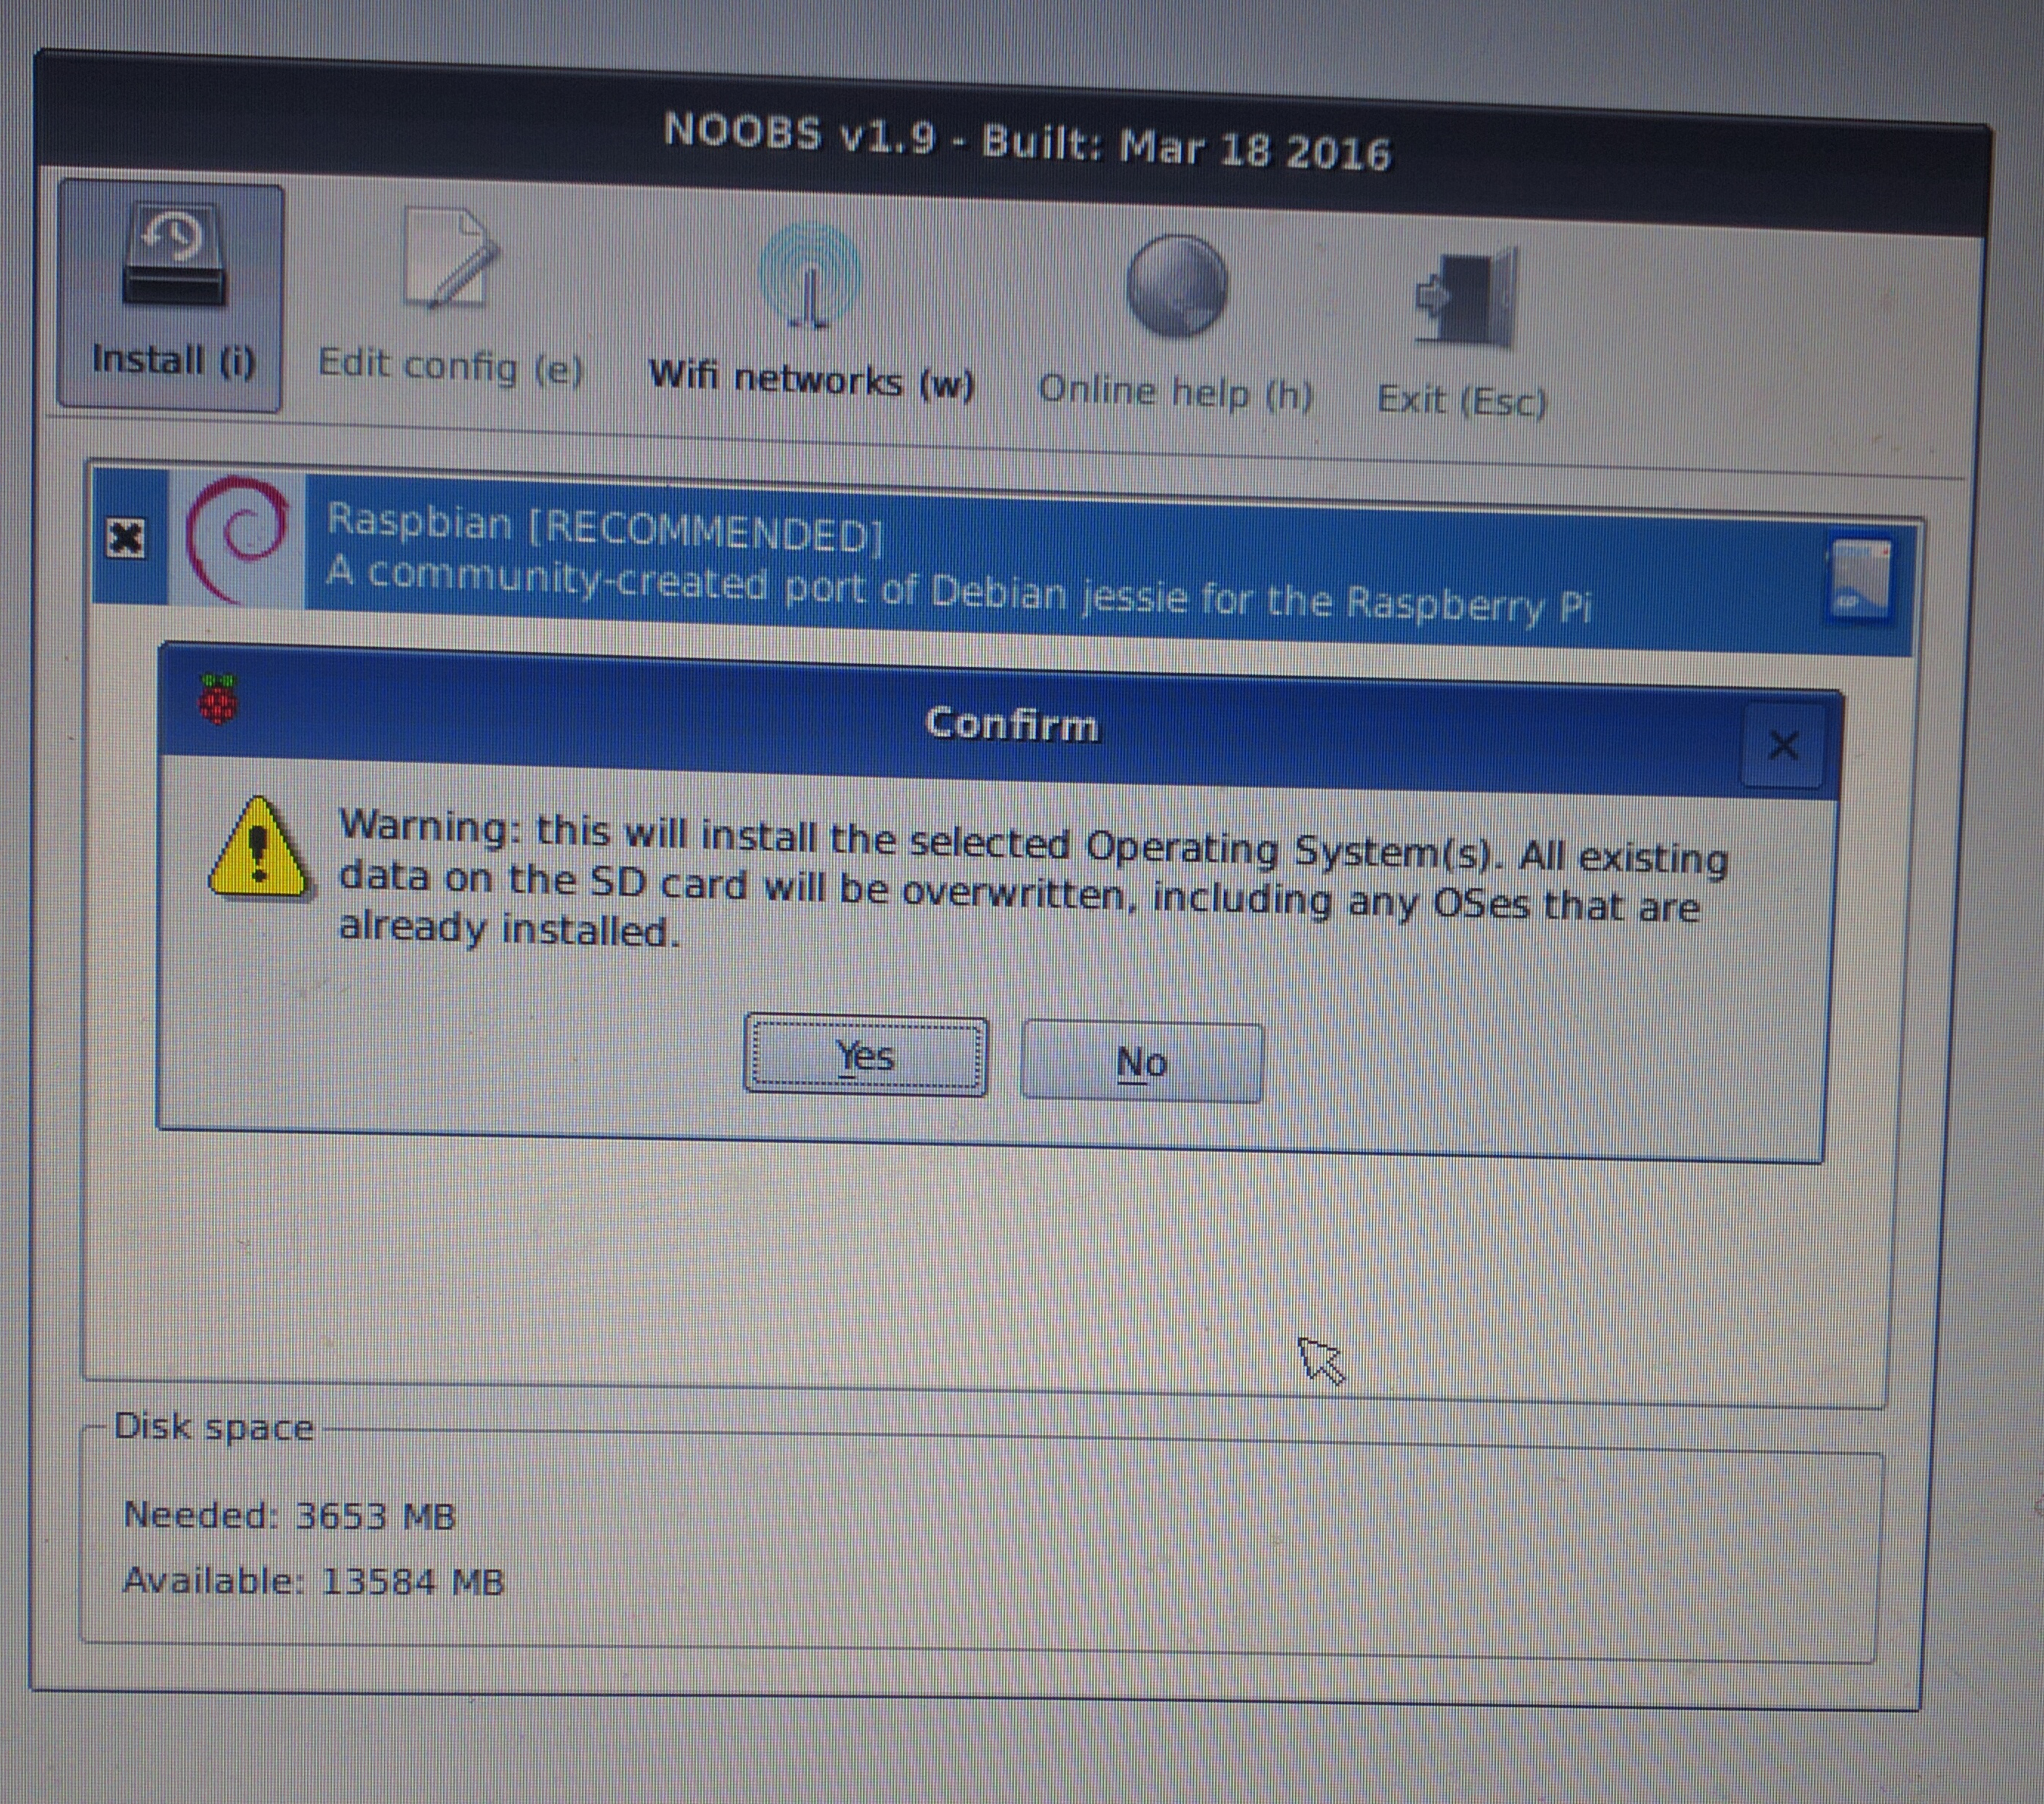
\includegraphics[height=1.75in]{pi_images/setup/OpeningScreen2.jpg}}
\afterfig

On that screen, select "Yes" in order to confirm the installation of Raspbian. \textbf{NOTE:} the installation process will take about 15 minutes\footnoteref{SdClass} to complete.

Once the installation is complete, a dialog will pop up saying that the OS has been installed successfully, click "OK" to finish the installation. 

\beforefig
\centerline{\includegraphics[height=1	in]{pi_images/setup/OpeningScreen3.jpg}}
\afterfig

The Pi will then restart. Once the standard Raspbian graphical desktop opens you may continue.

\end{enumerate}

\section{Configuring your Pi}

\index{configuration!Raspberry Pi}
\index{Raspberry Pi configuration}

\begin{enumerate}
	
	\item \textbf{Connecting to the Internet}

Now that you have your OS installed you need to connect your Pi to the network. Click on the icon in the upper-right of the screen and select the proper network name for your connection.

\beforefig
\centerline{\includegraphics[height=1	in]{pi_images/setup/NoInternet.jpg}}
\afterfig
	
If the network you select requires a password (shared secret) you will be prompted to enter the password. Once the correct password has been entered you will be connected to the network.

Note that some WiFi networks require you to authenticate using a user id and password entered in your browser. To verify that you have an Internet connection open the Epiphany browser (Menu|Internet|Epiphany) and attempt to access a web site.

\item \textbf{Changing the Default Password}

You should now change the password for your Pi to a unique password that only you know.\footnote{The default password for the \texttt{pi} account is \texttt{raspberry}} Open up a terminal window using the terminal icon located with the set of icons in the upper-left corner of the screen:

\index{setting!password}
\index{password!changing}

\beforefig
\centerline{\includegraphics[height=1 in]{pi_images/setup/Terminal.jpg}}
\afterfig

Once the terminal opens, enter the command \textbf{\texttt{sudo~raspi-config}}. Note that you \textbf{must press the \texttt{Enter}} key after typing a terminal command.\footnote{For the remainder of this setup guide we'll skip the reminder to press the \textbf{Enter} key after typing each command. Just remember it is needed.} After entering the command your screen should look like this:

\beforefig
\centerline{\includegraphics[height=1 in]{pi_images/setup/configuration_tool_menu.jpg}}
\afterfig

This is the main \textbf{Configuration Tool} menu. 

\beforefig
\centerline{\includegraphics[height=1 in]{pi_images/setup/change_password_choice.png}}
\afterfig


With \textbf{Change User Password} (the first option) selected, press the \textbf{Enter} key. Your screen should now look like this:

\beforefig
\centerline{\includegraphics[height=1.0 in]{pi_images/setup/ChangePassword2.jpg}}
\afterfig

Press \textbf{Enter} again to proceed to the password change screen. The screen will return to the terminal prompt which will now prompt you to enter the new password.

As you type your password \textit{you will not see any characters being displayed on the screen.} Press \textbf{Enter} once you have typed your desired password.

\beforefig
\centerline{\includegraphics[height=1.5 in]{pi_images/setup/ChangePassword3.jpg}}
\afterfig

You will be prompted to re-enter your password. Once you complete the second password entry, and press \textbf{Enter}, a message will be displayed telling you that your password has been changed. Press \textbf{Enter} one more time and you will be returned to the \textbf{Configuration Tool} menu.

\item \textbf{Setting the Boot Mode}

By default, when the Pi starts up it will launch the graphical environment and log into the \texttt{pi} user account. This means that any user who boots your Pi is logged in, bypassing your password setting. You should change this so that a login screen is presented when the Pi boots.

\index{setting!boot mode}
\index{boot mode!setting}

From the \textbf{Configuration Tool} menu, which should be the current menu after completing the earlier password setting step, use the down arrow to select option three, \textbf{Boot Options}, and press \textbf{Enter}.

\beforefig
\centerline{\includegraphics[height=1.5 in]{pi_images/setup/boot_options_choice.png}}
\afterfig

You will be presented with a menu of user interface options. Press \textbf{Enter} to choose the \textbf{B1 Desktop / CLI} option (the first option).

\beforefig
\centerline{\includegraphics[height=1.5 in]{pi_images/setup/desktop_cli_choice.png}}
\afterfig

\newpage 

Next, use the down arrow to choose the \textbf{B3 Desktop} option and press \textbf{Enter}. This will set the Pi to boot into the graphical environment, presenting a login screen to the user.

\beforefig
\centerline{\includegraphics[height=1.0 in]{pi_images/setup/desktop_login_boot_choice.png}}
\afterfig

Again, you will return to the \textbf{Configuration Tool} menu.

% \newpage

\item \textbf{Changing the Locale}

From the \textbf{Configuration Tool} menu use the down arrow to select option four, \textbf{Localisation Options}, and press \textbf{Enter}.

\index{setting!locale}
\index{locale!choosing}

\beforefig
\centerline{\includegraphics[height=1.5 in]{pi_images/setup/localisation_options_choice.png}}
\afterfig

Next choose the \textbf{Change Locale} option and press \textbf{Enter}.

\beforefig
\centerline{\includegraphics[height=0.75 in]{pi_images/setup/change_locale_choice.png}}
\afterfig

Using the up and down arrow keys scroll through the list of locales and highlight the \textbf{en\_US ISO-8859-1} line. Make sure the item is selected (e.g. shows an asterisk next to the item). You toggle the selection (asterisk) by pressing the spacebar while the line is highlighted.

\beforefig
\centerline{\includegraphics[height=1.5 in]{pi_images/setup/locale_en_us_iso.png}}
\afterfig

Use the \textbf{Tab} key to highlight the \textbf{Ok} option and press the \textbf{Enter} key.

You will then be shown a screen where you choose the default locale. Use the up and down arrow keys to highlight the \textbf{en\_US} option and press \textbf{Enter}.

\beforefig
\centerline{\includegraphics[height=1.5 in]{pi_images/setup/configure_default_locale.png}}
\afterfig

Again, you will return to the \textbf{Configuration Tool} menu.

% \newpage

\item \textbf{Changing the Timezone}

The next step is to set the timezone of your Pi. From the \textbf{Configuration Tool} menu select option four again, \textbf{Localisation Options}, and press \textbf{Enter}. Next, select option \textbf{I2, Change Timezone} and press \textbf{Enter}.

\index{setting!timezone}
\index{timezone!setting}

\beforefig
\centerline{\includegraphics[height=0.75 in]{pi_images/setup/ChangeTimezone1.jpg}}
\afterfig

Use the up and down arrows to navigate to the \textbf{US} option under the \textbf{Geographic area} and press \textbf{Enter}.

\beforefig
\centerline{\includegraphics[height=1.5 in]{pi_images/setup/ChangeTimezone2.jpg}}
\afterfig

Next, select the \textbf{Eastern} option under the \textbf{Time zone} and press \textbf{Enter}.

\beforefig
\centerline{\includegraphics[height=1.5 in]{pi_images/setup/ChangeTimezone3.jpg}}
\afterfig

\newpage

\item \textbf{Changing the Keyboard Layout}

The next step is to set the keyboard layout for your Pi. From the same menu screen select option four again, \textbf{Localisation Options}, and press \textbf{Enter}. Next, select option \textbf{I3, Change Keyboard Layout} and press \textbf{Enter}.

\index{setting!keyboard layout}
\index{keyboard layout!setting}

\beforefig
\centerline{\includegraphics[height=0.75 in]{pi_images/setup/change_keyboard_layout_choice.png}}
\afterfig

% \newpage

Using the up and down arrow keys select the \textbf{Generic 104-key PC} option and press \textbf{Enter}.

\beforefig
\centerline{\includegraphics[height=1.5 in]{pi_images/setup/keyboard_choice_generic.png}}
\afterfig

You will be asked to choose the keyboard layout language. Use the up and down arrows to select the \textbf{English (US)} option and press \textbf{Enter}.

\beforefig
\centerline{\includegraphics[height=1.5 in]{pi_images/setup/keyboard_language_choice_english.png}}
\afterfig

You will then be asked to configure the \textit{AltGr} setting. Using the up and down arrows choose the \textbf{The default for the keyboard layout} option and press \textbf{Enter}.

\beforefig
\centerline{\includegraphics[height=1.5 in]{pi_images/setup/keyboard_layout_choice_default_altgr.png}}
\afterfig

Next you will be asked to configure the \textit{Compose key} setting. Using the up and down arrows choose the \textbf{No compose key} option and press \textbf{Enter}.

\beforefig
\centerline{\includegraphics[height=1.5 in]{pi_images/setup/keyboard_layout_default_compose_key.png}}
\afterfig

Finally you will be asked whether you want to enable the \textit{Ctrl-Alt-Backspace key combination} function. Using the \textbf{Tab} key select the \textbf{No} option and press the \textbf{Enter} key.

\beforefig
\centerline{\includegraphics[height=0.75 in]{pi_images/setup/keyboard_layout_default_altctlbksp.png}}
\afterfig

You will be brought back to the \textbf{Configuration Tool} menu again. You may exit the menu by using the \textbf{Tab} key to select the \textbf{Finish} option and pressing \textbf{Enter}. 

\textit{If you changed the boot option as suggested in an earlier step} you will be asked whether or not the Pi should be rebooted. If asked, you may use the \textbf{Tab} key to choose the \textbf{No} option and press the \textbf{Enter} key.

\beforefig
\centerline{\includegraphics[height=0.75 in]{pi_images/setup/reboot_request_screen.jpg}}
\afterfig

At this point you will return to the terminal prompt.

\item \textbf{Updating the Packages}

Now we need to update several packages on the Pi. These packages represent programs that are installed on the Pi as part of the NOOBS setup process but may have been updated since the NOOBS installer was created.

\index{updating system packages}
\index{system updates}

Enter the command \textbf{\texttt{sudo~apt-get~update}} into the terminal. This process will take a couple of minutes to run.

\beforefig
\centerline{\includegraphics[height=1.5 in]{pi_images/setup/UpdatePackages1.jpg}}
\afterfig

\newpage

Next, enter the command \textbf{\texttt{sudo~apt-get~upgrade}} into the terminal. You will be asked if you want to continue the upgrade. Type the letter \textbf{\texttt{Y}} and press the \textbf{Enter} key to continue.  \textit{This process may take 15 minutes or more to complete depending on your Internet connection speed.}\footnoteref{SdClass}

\beforefig
\centerline{\includegraphics[height=1.5 in]{pi_images/setup/UpdatePackages2.jpg}}
\afterfig

\item \textbf{Installing Eclipse}

\index{Eclipse installation}

A popular Java Integrated Development Environment (IDE) is Eclipse. To install Eclipse enter the command \textbf{\texttt{sudo~apt-get~install~eclipse}} on the terminal's command line. Again, you will be asked if you want to continue, and again you will type the letter \textbf{\texttt{Y}} and press the \textbf{Enter} key to continue. This step may take 20 minutes or more\footnoteref{SdClass} to complete.

\index{Eclipse!installation}
\index{install!Eclipse}

\beforefig
\centerline{\includegraphics[height=1.5 in]{pi_images/setup/UpdatePackages3.jpg}}
\afterfig

\item \textbf{Configuring Java}

To setup the proper Java compiler, enter the command \textbf{\texttt{sudo~update-alternatives~--config~javac}} and then enter the number next to the option containing the term \textbf{oracle}. In the example shown below this is option number 2.

\beforefig
\centerline{\includegraphics[height=1.5 in]{pi_images/setup/UpdatePackages4.jpg}}
\afterfig

To setup the proper Java runtime, enter the command \textbf{\texttt{sudo~update-alternatives~--config~java}} and again, enter the number next to the option containing the term \textbf{oracle}. In the example shown below this is option number 2.

\beforefig
\centerline{\includegraphics[height=1.5 in]{pi_images/setup/UpdatePackages5.jpg}}
\afterfig

%\item \textbf{Java-GPIO Setup Script}

%At this point your instructor will provide you with a script to be run that creates a Java configuration that will allow you to run Java programs %that use the GPIO header. Refer to the information from you instructor to complete this step.

\end{enumerate}

\iffalse % Comment out this section since there is no need to run Java as root for PiLib anymore

\section{Configuring Eclipse}

Now we will configure Eclipse. First open Eclipse, which can be found under the Programming section of the Pi menu.

\index{Eclipse!configuration}
\index{configure!Eclipse}

\beforefig
\centerline{\includegraphics[height=2.5 in]{pi_images/setup/ConfigureEclipse1.jpg}}
\afterfig

Once Eclipse opens, you will be asked which Workspace you would like to use. The default workspace is what we will be using, so just click \textbf{OK} to continue.

\beforefig
\centerline{\includegraphics[height=2.5 in]{pi_images/setup/ConfigureEclipse2.jpg}}
\afterfig

Next, click on the \textbf{Workbench} option to continue to Eclipse's Java workbench.

\beforefig
\centerline{\includegraphics[height=1.5 in]{pi_images/setup/ConfigureEclipse3.jpg}}
\afterfig

Under the \textbf{Window} menu, click on the \textbf{Preferences} option on the bottom.

\beforefig
\centerline{\includegraphics[height=3.0 in]{pi_images/setup/ConfigureEclipse4.jpg}}
\afterfig

Expand the \textbf{Java} selection by clicking the plus sign \textbf{+} next to it, and select the \textbf{Installed JREs} option. Select the \textbf{jdk-8-oracle} JRE and click the \textbf{Duplicate} button.

\beforefig
\centerline{\includegraphics[height=3.0 in]{pi_images/setup/ConfigureEclipse5.jpg}}
\afterfig

A screen will pop up allowing you to edit the JRE definition before you create the duplicate. Change the \textbf{JRE name:} by removing the \textbf{(1)} (including the space) and appending \textbf{\texttt{-root}}. Next, under the \textbf{Default VM arguments}, add \textbf{\texttt{--run-as-root}}. Verify your changes by comparing them to the screenshot below:

\beforefig
\centerline{\includegraphics[height=3.0 in]{pi_images/setup/ConfigureEclipse6.jpg}}
\afterfig

Click the \textbf{Finish} button and make sure that the checkbox next to the JRE that you just created (with the name ending with -root) is not checked. To complete the process and click the \textbf{OK} button.

\beforefig
\centerline{\includegraphics[height=2.5 in]{pi_images/setup/ConfigureEclipse7.jpg}}
\afterfig

\fi % Comment out this section since there is no need to run Java as root for PiLib anymore

%\newpage

\section{Setup the PiLib Server}\label{setupPiLibServer}

\index{PiLib}
\index{library!PiLib}
\index{PiLib!Server program}

To simplify working with the GPIO interface and breadboard components we will use a library, \textbf{PiLib}, that provides two features:

\index{PiLib server!installation}
\index{install!PiLib server}

\begin{enumerate}
	\item Allows a library of functions available to our Java program to control the LEDs and react to the buttons being pressed
	\item Provides a web-based view of the current GPIO operations. This allows you to view the configured LEDs and buttons as well as see each LED's state (on/blink/off) and interact with buttons (by pressing them via a mouse click) 
\end{enumerate}

The PiLib library is made up of two parts, the server program and the client library. The client library will be included in each lab and will be described in the lab appendix. The server has to be installed on your Pi and then started each time you want to run a program that uses the client library to interact with the breadboard (LEDs and buttons).

Your instructor will give you the address of a website to download the \textbf{\texttt{PiLibServerDist.tar.gz}} file. I recommend for convenience you place that file in your home directory. Once you've placed the file in your home directory, access a terminal and type the following commands:

\texttt{\$ cd} \linebreak
\texttt{\$ tar xvzf PiLibServerDist.tar.gz}

\textit{Note that the} \texttt{\$} \textit{(dollar sign) is the terminal prompt.} You do not type the \texttt{\$}. Also, your terminal prompt may look different than a plain dollar sign.

The first command (\texttt{cd}) assures your terminal is accessing your home directory. You don't need to type the first command if your terminal automatically opens in your home directory.

The second command will create a directory called \textbf{\texttt{PiLibServerDist}} that contains the server program and a script to run it.

See the section \textbf{\textit{Starting the PiLib Server}} in the labs appendix for information on using the PiLib Server.

\section{Your Pi Is Configured}

\textbf{Congratulations!} Your Pi is now setup with an up-to-date operating system and configured so that it is ready for you to complete the course labs.

\index{Login screen}

Remember that the next time you start up your Pi it will prompt you for a login id and password. The login account name, unless you change it, is \textbf{\texttt{pi}}. The password is whatever you set it to earlier in this setup process. (If you don't change it, the default password is \texttt{raspberry})

Here is what the login screen looks like:

\beforefig
\centerline{\includegraphics[height=1.0 in]{pi_images/setup/login_screen.jpg}}
\afterfig

Fill in the user id and password then press \textbf{\texttt{Log In}} and you will see the graphical desktop.
%% LaTeX source for ``Introduction to Computer Science (Java/Pi Edition)''
% Copyright (c) 2015- David S. Read, All Rights Reserved

\chapter{Raspberry Pi Labs}


\section{A Platform for Experimentation and Learning}

\index{Raspberry Pi}

In the early days of home computing the machines were very basic and packaged software was limited to 
some simple games and very basic office tools. Many computers were targeted at hobbyists who would 
write their own programs. There was no Internet full of information and media to consume,
so the computer was a device for active experimentation rather than passive entertainment.

Over the years computers have become more sophisticated, expensive and central to many household operations
(such as paying bills) while the Internet grew up and provided a nearly inexhaustible amount
of content and functionality to use and explore. Computers transitioned from experimental
workshops for hobbyists to a common appliance, leveraged by all family members for a variety
of purposes.

The Raspberry Pi\footnote{Another small computing device good for experimentation is the Arduino} was created
by several individuals who work in the computer science field and felt that having an affordable
computer for basic experimentation would be of interest to the general public. It appears they were correct
given the increasing popularity of the Pi, including its use in production environments.

This chapter will introduce you to the Raspberry Pi 3 while providing a series of lab exercises for you
to complete. The labs are intended to meet two goals: 

\begin{itemize}
	
\item Have some fun building simple circuits and interacting with them using programs you write.

\item Reinforce the principles of object oriented programming by associating physical objects (LEDs and buttons)
with virtual objects (instances of classes) and seeing how the attributes and behaviors in the
virtual environments manifest in the physical world.

\end{itemize}

\section{Introducing the Raspberry Pi 3}

\begin{figure}[H]
	\centering
	%	\begin{mdframed}
	\includegraphics[height=3.50in]{pi_images/Raspi-3-Layout.jpg}
	%	\end{mdframed}
	\caption{The Raspberry Pi 3 with key components labeled}
	\label{fig:raspberrypi3}
\end{figure}

Hereafter I'll generally refer to the Raspberry Pi as the Pi.

The Pi is a great environment for learning about computing devices and programming. It has several key 
advantages over programming on a general computer system:

\begin{itemize}
	\item it is a relatively inexpensive full-featured computing device
	\item it is capable of running a variety of commodity software development tools
	\item it provides access to input and output signals via its General Purpose Input/Output (GPIO) connector
\end{itemize}

The first two advantages are straightforward. The GPIO interface deserves a little more definition.

\section{GPIO - General Purpose Input/Output}

\index{GPIO}

We often interact with computers using screens, keyboards and mice. Sometimes we use other input devices
such as scanners and drawing tablets. We can output information to printers or other computers across a network.
Often that is the limit of our direct computer interactions. However, inside the computer there are
a variety of electrical signals being used to communicate between the computer's components. These core components, which
we discussed in chapter 0, include the CPU, main memory, disk drives and network cards.

Typically we don't have any easy way to interface directly with these types of signals. For example, many computers
have a light which indicates when the disk drive is being accessed. Generally we don't have access to that
electrical signal, we just see the light flickering.

The Pi's J8 GPIO interface allows us to attach devices to the Pi and use them for input and output. For example
we can connect an LED to a GPIO pin and then write a program that turns the LED on and off. Similarly we
can connect a button to another GPIO pin and use the button as a signal for a program to take a certain
action when the button is pressed.

Figure~\ref{fig:j8header} is a close-up of the GPIO J8 40-pin interface that depicts several pin numbers (these are \textbf{\textit{not}} the GPIO numbers, which we'll see shortly). The pins are simply numbered sequentially:

\begin{figure}[H]
	\centering
	%	\begin{mdframed}
	\includegraphics[height=1.30in]{pi_images/j8header-photo-transparentbg.png}
	%	\end{mdframed}
	\caption{Raspberry Pi 3's J8 Header with several pins labeled}
	\label{fig:j8header}
\end{figure}

To allow our programs to interface with the pins we need a way to identify which physical pins we want to 
control from within our program. The Pi uses a numbering scheme where the controllable pins are assigned
a GPIO number. Unfortunately different versions of the Pi have used different GPIO numbering schemes. 

To
deal with this numbering confusion, the Java library we will be using, known as Pi4J\footnote{Short for \textbf{Pi \textit{for} Java}. You can read more about this library at \url{http://pi4j.com/}}, assigns consistent GPIO numbers to the
pins regardless of which Pi device we are using. 

\pagebreak

Figure~\ref{fig:pi4jgpio} depicts the GPIO numbers assigned by the Pi4J library. We will use these numbers throughout the chapter. You'll want to keep 
track of this figure for quick reference when you are building the lab circuits.

\begin{figure}[H]
	\centering
	%	\begin{mdframed}
	\includegraphics[height=6.0in]{pi_images/j8header-2b-dsr-flat.png}
	%	\end{mdframed}
	\caption{The Pi's J8 pin and row numbers with the Pi4J GPIO numbering}
	\label{fig:pi4jgpio}
\end{figure}

The bold numbers at the extreme right and left of the diagram are the GPIO numbers. The numbers in green give the row number of the pin (useful when we are describing the wiring for a lab project since they line up with the row numbers printed on the breadboard). The small vertically-oriented (sideways) numbers are the physical pin numbers which we generally won't be concerned with.

\pagebreak

\section{Breadboards - Easy Wiring}

\index{breadboard}

In order to create our lab project circuits, we will use
a breadboard which allows us to easily connect different
electrical devices to the Pi without worrying about soldering. A breadboard has a set of electrically-connected
holes into which we insert jumper wires, LEDs,
buttons, etc.

Figure~\ref{fig:breadboard} is a picture of the breadboard we will be using for the labs:

\begin{figure}[H]
	\centering
	%	\begin{mdframed}
	\includegraphics[height=2in]{pi_images/half-size-breadboard-600x600_grande.jpg}
	%	\end{mdframed}
	\caption{Standard half-size breadboard}
	\label{fig:breadboard}
\end{figure}

Note that there are 14 columns of holes. The first and last two columns are special (marked with + and -). The center set of 10 columns are labeled a-j in two groups, a-e and f-j. There are 30 rows of holes available for columns a-j.

Let's consider how the breadboard is wired internally. The connection points for the first and last two columns (labeled + and -) are electrically connected by column. The connection points in the columns labeled a-e and the ones in columns f-j are connected horizontally in groups of 5. For example a connection to point a1 is connected to holes b1, c1, d1 and e1. Similarly f1 is connected to g1, h1, i1 and j1.

These images below attempt to clarify how the holes are tied together:

%\beforefig
%\centerline{\includegraphics[height=2.00in]{pi_images/Breadboard_Remarked_grande.png}}
%\afterfig

\iffalse % comment out images displayed one above the other

\beforefig
\centerline{\includegraphics[height=2.0in]{pi_images/verticalpower.png}}
\afterfig

\beforefig
\centerline{\includegraphics[height=2.0in]{pi_images/horizontal-rows.png}}
\afterfig

\fi % end of skipping images

\begin{tabular}{p{0.4\textwidth} p{0.3\textwidth}}
	\vspace{0pt} \includegraphics[height=1.4in]{pi_images/verticalpower.png} &
	\vspace{0pt} \includegraphics[height=1.4in]{pi_images/horizontal-rows.png}
\end{tabular}



This layout will make more sense once you complete the first lab 
and put together your initial set of components.

\section{Connecting the Pi and a Breadboard}

It may have occurred to you that there is no way to directly attach the breadboard to the Pi. For that we need two more pieces of equipment: a breakout board and ribbon cable.

A breakout board\footnote{Also called a cobbler breakout} provides a way to connect the 40 pins from the J8 GPIO interface to separate sets of holes on the breadboard. A ribbon cable then allows us to connect the breakout board to the Pi.

Figure~\ref{fig:piwithbreadboard} shows the entire setup, connecting the Pi to the ribbon cable, which attaches to the breakout board which is installed on the breadboard. This is the basic workbench we will be using for our Pi labs.

\begin{figure}[H]
	\centering
	%	\begin{mdframed}
	\includegraphics[height=2.5in]{pi_images/breadboard-cobbler-pi.jpg}
	%	\end{mdframed}
	\caption{Raspberry Pi, ribbon cable, breakout board and breadboard}
	\label{fig:piwithbreadboard}
\end{figure}

\section{Electronics - keeping it basic}

This book is not intended to make you an electrical engineer. Each lab will clearly spell out all of the 
connections you need to make in order to setup the 
breadboard for the specific assignment. Your job will be
to write programs. In this case the programs will control
(or be controlled by) devices attached to the Pi via the breadboard.

\pagebreak

The basic components you will be working with are:

\begin{enumerate}
\item \textbf{Jumper cables}

\index{jumper cable}
\index{breadboard!jumper cable}

\beforefig
\centerline{\includegraphics[height=1.50in]{pi_images/breadboard-jumper-cables.jpg}}
\afterfig

Jumper cables have a pin at each end that are easily inserted into the breadboard holes. The cables are used to connect one set of holes to another set of holes. For example, when we need to connect an LED to a GPIO pin we will insert one end of a jumper cable into the same row as the GPIO pin and insert the other end of the jumper into a hole in the same row with the LED's wire.

\item \textbf{Resistors}

\beforefig
\centerline{\includegraphics[height=0.50in]{pi_images/resistor3-500x500.jpg}}
\afterfig

A resistor, as its name implies, resists the flow of electricity through a circuit. In our case we want to be sure that we do not damage the Pi or our LEDs with too high a current flow.

The resistors have two connecting wires whose orientation doesn't matter. When we list two holes on the breadboard for the resistor's wires to be inserted into, you can insert either end of the resistor into either hole.

\item \textbf{Buttons}

\index{button}
\index{breadboard!button}

\beforefig
\centerline{\includegraphics[height=0.70in]{pi_images/button_large.jpg}}
\afterfig

The buttons we will use are known as momentary contact buttons. This means that they only make contact (complete a circuit) while being held down. Our programs can then respond to the button being pressed when the Pi detects that a circuit has been completed by the button. Here is a diagram of how the switch is wired.

\beforefig
\centerline{\includegraphics[height=0.70in]{pi_images/button_schematic.png}}
\afterfig

Like resistors, each button has two connection points and their orientation does not matter. When we list two holes on the breadboard for the button's terminals to be inserted into, you can insert either end of the button into either hole.

\iffalse % Ignoring this information for the 4 connection buttons

\beforefig
\centerline{\includegraphics[height=1.00in]{pi_images/Push-Switch-fs8-1024x269.png}}
\afterfig

The buttons we will use are known as momentary contact buttons. This means that they only make contact (complete a circuit) while being held down. Our programs can then respond to the button being pressed when the Pi detects that a circuit has been completed by the button. Above is a picture of a button with a diagram of how the switch is wired.

Don't worry about the A-B-C-D labeling yet. We'll formally work through connecting the switch in the first lab to use one. It turns out the orientation of the button will matter when we place it on the breadboard.

\textbf{\underline{Take note that the orientation of buttons matters}}. Looking at the bottom of the buttons you'll note that they have four contacts. In one direction the contacts are closer together than in the other. Looking at the diagram above, the A-D and B-C contacts are more widely spaced than the A-B and C-D contacts.

For our labs, \textbf{when inserting the buttons into the breadboard you will need to place them so that the more widely spaced contacts are arranged on opposite sides of the breadboard's center line}. That is, A-B goes on one side of the center line and C-D go on the other. \textit{If you're unsure about their placement, check with your instructor.}

\fi % End of ignored section discussing the 4 contact buttons

\item \textbf{LEDs}

\index{LED}
\index{breadboard!LED}

\beforefig
\centerline{\includegraphics[height=1.50in]{pi_images/led_2.jpg}}
\afterfig

The acronym LED stands for Light Emitting Diode. A key term is diode. A diode is sensitive to the direction of electrical current flow. There is a right way and wrong way to connect one.

The anode end must tie to the positive side of the circuit while the cathode end must tie to the negative side. You can identify the anode on the LED since it has a longer connector wire. 

If the wire lengths are too close to differentiate you can also look for a flat spot on one side of the LED. The wire nearest the flat spot will be the cathode.


\end{enumerate}

Those are the only components we will work with for this set of labs. They extend our keyboard and screen with new ways to interact with the computer, pressing a button to provide input and lighting an LED to provide output.

\section{PiLib - classes for components}

\index{PiLib}
\index{library!PiLib}

We've toured through the hardware we'll be using. Now we need to describe the software that will allow us to turn on LEDs and detect button presses.

\textbf{\underline{Widget Control}} \newline

The library, called PiLib, is comprised of several classes that are used to represent the physical components. Developers often call such components widgets. The base class in PiLib for interacting with
physical components is Widget. This class is abstract so you won't be creating any instances of it.

Each Widget subclass will represent a physical component such as an LED or button. Since any physical component must be connected to a GPIO pin in order to be accessible from the Pi, the Widget class has an attribute representing the GPIO number (as depicted in the earlier Pi4J numbering diagram).

Below is an overview of the specific Widget subclasses that you will be using. The first time each one is used in a lab we will go into more detail.

Also, note that there is complete JavaDoc for PiLib. It can be found with the library itself as well as at:  \url{https://monead.com/iot/PiLibClient/}.

\index{PiLib!JavaDoc location}

The four classes of interest are:

\begin{enumerate}
	\item \textbf{Widget} \newline
	This represents any widget. Each of the classes listed below are subclasses of Widget. The Widget class has a few special static methods including \textbf{\texttt{gpioReset()}} which removes old GPIO pin mappings.
	
\index{Widget class}
\index{PiLib!Widget class}
\index{gpioReset() method}
\index{Widget.gpioReset() method}
\index{PiLib!gpioReset() method}

	You'll normally want to call that at the beginning of your program to be sure there aren't any old GPIO pin mappings configured. You call the method by simply including the statement \textbf{\texttt{Widget.gpioReset();}} in your program before creating your mappings. You may also call it at the end of your program to remove mappings and leave the environment in a clean state. 
	
	The Widget class also defines the static methods \textbf{\texttt{turnOffAllLeds()}}, \textbf{\texttt{turnOnAllLedsSolid()}} and \textbf{\texttt{turnOnAllLedsBlink()}} which are convenience methods to quickly set all the LEDs to a specific mode.

\index{turnOffAllLeds() method}
\index{Widget.turnOffAllLeds() method}
\index{PiLib!turnOffAllLeds() method}
\index{turnOnAllLedsSolid() method}
\index{Widget.turnOnAllLedsSolid() method}
\index{PiLib!turnOnAllLedsSolid() method}
\index{turnOnAllLedsBlink() method}
\index{Widget.turnOnAllLedsBlink() method}
\index{PiLib!turnOnAllLedsBlink() method}
	
	For controlling \texttt{BinaryLed} instances (see below) the \textbf{\texttt{Widget.setBinaryValue()}} method takes an \texttt{int} parameter which is the value you want displayed by the \texttt{BinaryLed} instances.
	
\index{BinaryLed class}
\index{PiLib!BinaryLed class}

	If you review the JavaDoc for the Widget class you will see that it also contains a method called \texttt{shutdown()}. You will rarely use this method since it shuts down the PiLibServer. \textit{You cannot make further use of the library methods (for instance you can't call methods on the Led instances) once the  \texttt{shutdown()} method is called until you restart the PiLibServer program.} 

	\item \textbf{Button} \newline
	This represents the operations and attributes that are allowed for a button. The operations are detecting that the button has been pressed, getting a count of times it has been pressed and resetting the button's counter.
	
	The three methods of interest provided by the Button class are \textbf{\texttt{getPressCount()}}, \textbf{\texttt{clearPressCount()}} and \textbf{\texttt{waitForPress()}}. See the JavaDoc for details.

\index{Button class}
\index{PiLib!Button class}
\index{getPressCount() method}
\index{Button.getPressCount() method}
\index{PiLib!Button.getPressCount() method}
\index{clearPressCount() method}
\index{Button.clearPressCount() method}
\index{PiLib!Button.clearPressCount() method}
\index{waitForPress() method}
\index{Button.waitForPress() method}
\index{PiLib!Button.waitForPress() method}
	
	\item \textbf{Led} \newline
	This represents the operations that are allowed for an LED. The operations include turning the LED off, turning it on and making it blink. There are no additional attributes associated with an LED.
	
	The three methods of interest provided by the Led class are \textbf{\texttt{turnOff()}}, \textbf{\texttt{turnOnSolid()}} and \textbf{\texttt{turnOnBlink()}}. See the JavaDoc for details.
					
\index{Led class}
\index{PiLib!Led class}
\index{turnOff() method}
\index{Led.turnOff() method}
\index{PiLib!Led.turnOff() method}
\index{turnOnSolid() method}
\index{Led.turnOnSolid() method}
\index{PiLib!Led.turnOnSolid() method}
\index{turnOnBlink() method}
\index{Led.turnOnBlink() method}
\index{PiLib!Led.turnOnBlink() method}
	
	\item \textbf{BinaryLed} \newline
	This represents an LED that is being used in a group
	with other LEDs as a way to represent binary numbers. Don't worry about binary if you aren't familiar with it. We'll cover it in a later lab. The \texttt{Widget.setBinaryValue()} method (described above) is used to make displaying of binary numbers easy.
	
	\texttt{BinaryLed} is a subclass of \texttt{Led} meaning it inherits the \texttt{Led} class's methods \textbf{\texttt{turnOff()}}, \textbf{\texttt{turnOnSolid()}} and \textbf{\texttt{turnOnBlink()}}. See the PiLib JavaDoc for details.
					
\index{BinaryLed class}
\index{PiLib!BinaryLed class}
\index{turnOff() method}
\index{BinaryLed.turnOff() method}
\index{PiLib!BinaryLed.turnOff() method}
\index{turnOnSolid() method}
\index{BinaryLed.turnOnSolid() method}
\index{PiLib!BinaryLed.turnOnSolid() method}
\index{turnOnBlink() method}
\index{BinaryLed.turnOnBlink() method}
\index{PiLib!BinaryLed.turnOnBlink() method}
	
\end{enumerate}

The classes that you will use in your programs send commands to a server program. That program must be running on your Pi. The server, \textbf{PiLibServer}, needs special permissions in order to access the GPIO pins. See the section, \textbf{\textit{Starting the PiLib Server}} for information in using the PiLib server program.

\textbf{\underline{Utilities}} \newline

In addition to classes for controlling the widgets, PiLib has several utility methods to make working with the Pi and interacting with users a little simpler. Each of these methods is in the \textbf{\texttt{Utility}} class.

\begin{enumerate}
	\item \textbf{Collecting user input} \newline
	Many labs require our program to ask the user for information that must be supplied using the keyboard. Java makes it fairly easy to read input from the keyboard, however there is a redundant set of code that has to be written each time we want to get another piece of information.
	
	To simplify keyboard input, the \texttt{Utility} class contains the method \textbf{\texttt{readKeyboardLine()}}. The method waits for the user to type some characters and press the \textbf{Enter} key. Once the user presses \textbf{Enter} the method returns a \textbf{String} containing any characters the user typed prior to pressing \textbf{Enter}.
	
	Here is a simple program that asks the user to enter their name, gets the information from the keyboard and then prints his or her response on the screen.
	
\beforeverb
\begin{verbatim}
import us.daveread.raspberrypi.gpio.lib.Utility;

public class DemokeyboardInput {
 public static void main(String[] args) {
  String name;

  System.out.print("What is your name? ");
  name = Utility.readKeyboardLine();

  System.out.println("You replied with the name " + name);
 }
}\end{verbatim}
\afterverb

Here is an example of what this would look like when it is run:

\beforeverb
\begin{verbatim}
What is your name? Dave
You replied with the name Dave
\end{verbatim}
\afterverb


	\item \textbf{Pausing Program Execution} \newline
	When you are working with the LEDs you will often need to have your program pause so that the LED stays on or off for a defined period of time. For instance, if you wrote a program to turn on an LED, the LED would turn off as soon as the program ended. If you want to have the LED stay on for a couple of seconds before the program ends (turning off the LED) you need a way to pause the program.
	
	The \texttt{Utility} class contains the method \textbf{\texttt{pause()}} which will cause the program to stop executing statements for a defined period of time. You tell the \texttt{pause()} method how long to pause by passing the number of milliseconds to pause as a parameter.
	
	Here is an example of using the \texttt{pause()} method to print out the message, \textit{Hello World! Glad to meet you.} one word at a time. The amount of time the program pauses is different between different words.
	
	The program pauses for 1 second (1000 milliseconds) after printing \textit{Hello}. It pauses one half-second after printing \textit{World!} Looking at the code you can see the other pause lengths being used. Give the program a try to experience how the output will be presented.
	
\beforeverb
\begin{verbatim}
import us.daveread.raspberrypi.gpio.lib.Utility;

public class DemoPause {
 public static void main(String[] args) {
  System.out.println("Hello");
  Utility.pause(1000);
  System.out.println("World!");
  Utility.pause(500);
  System.out.println("Glad");
  Utility.pause(1500);
  System.out.println("to");
  Utility.pause(250);
  System.out.println("meet");
  Utility.pause(750);
  System.out.println("you.");
  Utility.pause(1250);    
 }
}\end{verbatim}
\afterverb
	
\end{enumerate}

\section{Starting the PiLibServer}

If you have not installed the PiLib server please see the section \textbf{\textit{Setup the PiLib Server}} on page \pageref{setupPiLibServer} in the \textit{Raspberry Pi Setup} appendix.

\index{PiLib}
\index{library!PiLib}
\index{PiLib!Server program}

Whenever you want to use the PiLib server program you will use a terminal (accessing your home directory) and type the following command:

\textbf{\texttt{\$ PiLibServerDist/runServerSudo.sh}}

\textit{Note that the} \texttt{\$} \textit{(dollar sign) is the terminal prompt.} You do not type the \texttt{\$}. Also, your terminal prompt may look different than a plain dollar sign.

This command starts the server. Your screen should contain a message similar to:

\texttt{2016-06-16 10:37:55,869 [us.daveread.raspberrypi.gpio.lib.server.PiLibServer] [main] (PiLibServer.java:45) WARN  us.daveread.raspberrypi.gpio.lib.server.PiLibServer  - PiLib service ready}

You must leave the terminal open (running) while working on your Pi Lab program. You may close the PiLib Server by selecting the terminal and typing \textbf{\texttt{[Ctrl]C}}. That is, hold the [Ctrl] key and press the letter \textbf{C}.

\section{PiLib Server Web Control}

The PiLib Server supports a web-based interface for three purposes:

\begin{enumerate}
	\item Client library control
	\item Viewing the current GPIO configuration
	\item Interacting with the GPIO configuration
\end{enumerate}

\textbf{\underline{View Current GPIO Configuration}}

If you want to view the current configuration, use the following address in your browser (note that the PiLib server must be running when you do this):

\textbf{\texttt{\url{http://localhost:5162/PiLib}}}

If you are not running a program that has setup GPIO mappings then you will see an empty page containing the message, \textit{No widgets have been created} (figure~\ref{fig:servernowidget}). Otherwise you will see a graphical representation for each mapped LED and button (figure~\ref{fig:serverwithwidget}).

\begin{figure}[H]
	\centering
%	\begin{mdframed}
	\includegraphics[height=1.50in]{pi_images/PiLibServerNoWidgets.png}
%	\end{mdframed}
	\caption{PiLib Server web page with no widgets}
	\label{fig:servernowidget}
\end{figure}

\begin{figure}[H]
	\centering
	%	\begin{mdframed}
	\includegraphics[height=1.8in]{pi_images/PiLibServerWithWidgets.png}
	%	\end{mdframed}
	\caption{PiLib Server web page with widgets configured}
	\label{fig:serverwithwidget}
\end{figure}

You may find this view helpful when building your Pi labs since you can see what GPIOs are configured for which components as well as seeing the state of the LEDs and interacting with the buttons. If you have your project setup and LEDs aren't lighting when expected or button presses aren't being detected, you can use this web page to see if the issue is with components on the breadboard or with the program.

\textbf{\underline{PiLib Server Test Web Page}}

If you want to test out a GPIO configuration without writing Java code you can setup several simple arrangements of components. The web URL for this is:

\textbf{\texttt{\url{http://localhost:5162/PiLib/test}}}

You may use this web page (figure~\ref{fig:servertestpage}) to modify the GPIO Configuration, mapping LEDs and buttons to GPIO numbers as well as clearing old mappings or even shutting-down the PiLib server. This page is intended for basic testing of the GPIO server. You will probably not find it particularly useful as you work through the Pi lab exercises.

\begin{figure}[H]
	\centering
	%	\begin{mdframed}
	\includegraphics[height=1.8in]{pi_images/PiLibServerTestPage.png}
	%	\end{mdframed}
	\caption{PiLib Server test page (top of page)}
	\label{fig:servertestpage}
\end{figure}

\section{Wiring Tests}
\label{wiringTestDescription}
\index{PiLab Wiring Test}
\index{Wiring Test!PiLab}

\beforefig
\begin{wrapfigure}{r}{40mm}
	\centerline{\includegraphics[height=1in]{images/approved-151676_960_720.png}}
\end{wrapfigure}
\afterfig

Every Pi Lab project includes a test program to check that all of the components are properly connected and working. The class file will always be called \textbf{\texttt{WiringTest.java}}.

For each lab, after wiring your breadboard and connecting it to your Pi, you should open the \textbf{\texttt{WiringTest}} program and run it. Depending on the components being used for your lab the program will exercise each one.

Generally it will turn on all the LEDs and then, if the lab uses buttons, it will have you press each button in sequence and report that the press was detected.

\beforefig
\begin{wrapfigure}{l}{40mm}
\centerline{\includegraphics[height=1in]{images/exclamation-mark-red-md.png}}
\end{wrapfigure}
\afterfig

If one or more of the components aren't working when the \texttt{WiringTest} is run you will need to fix it. Here are the three most common issues I've seen which cause the test to fail:

\begin{itemize}
	\item The PiLib Server has not been started
	\item The ribbon cable connector which plugs into the Pi is loose or not aligned correctly
	\item The components are not wired correctly on the breadboard. A common wiring mistake is connecting resistors to the wrong power rail (such as connecting to 3V3+ when the connection should be to 3V3--).
\end{itemize}

Make sure that the \texttt{WiringTest} works before proceeding. Your own program won't work correctly if the test isn't working.

Now that we have discussed the PiLib client and server components as well as how to test our breadboard wiring, let's give it all a try with our first lab.


\clearpage

\section{Lab 1 - Part 1}

\textbf{Learning Goals}

\begin{enumerate}
	\item Create a working circuit with 1 LED controlled by a Java program running on the Pi
	\item Explore the Led class methods that allow us to control a physical LED
	\item Understand the relationship between virtual objects (instances of a class) and their physical counterparts
\end{enumerate}

\textbf{Overview}

You will use your breadboard to connect an LED to a GPIO pin. With this setup you will write a Java program which controls the LED. In a second part of the lab you will add a second LED and control both of them with a program.

\textbf{Breadboard Configuration}

\hfill

{\centering
\fbox{\begin{minipage}{300pt}
\textbf{\underline{WARNING:} NEVER connect or disconnect the breadboard's ribbon cable from your Raspberry Pi when the Pi is powered-up. NEVER change the wiring on your
breadboard when it is connected to your powered-up Raspberry Pi. \textit{You 
can do \underline{permanent damage} (including rendering your Pi unusable)
if you are changing connections while your Pi is running.} Your best bet is to do the wiring when your Pi is disconnected from a power source.}
\end{minipage}
}\par
}

\hfill

For each lab we'll provide two images of the configured breadboard. One image will depict the components using drawings that clearly show the connection points. The other image will be a photo of a completed breadboard to help you validate the overall arrangement of the components.

In addition to the images there will be a step by step set of connection instructions. If you are unsure of a connection, verify it with the instructor, TA or a classmate.

\pagebreak

\underline{Wiring Depiction}

\beforefig
\centerline{\includegraphics[height=2in]{pi_images/lab01images/PiLab01-1Light.png}}
\afterfig

\underline{Wiring Steps}

\textbf{Remember, your Pi must be disconnected from a power source while wiring the circuit.}

\begin{enumerate}
	\item Insert an LED anode (longer wire) into hole \textbf{d22}
	\item Insert the same LED's cathode into hole \textbf{d23}
	
	\item Insert a jumper from hole \textbf{a6} to hole \textbf{a22}
	
	\item Insert a resistor between hole \textbf{a23} and a \textbf{3V3--} (negative) hole adjacent to row 23.
	
	\item If your ribbon cable is not connected to the Pi and the breakout board, connect it now (making sure your Pi is disconnected from any power source)
\end{enumerate}

\underline{Completed Breadboard Picture}

\beforefig
\centerline{\includegraphics[height=2in]{pi_images/lab01images/PiLab01-1Light-photo.jpg}}
\afterfig

\underline{GPIO Assignments}

\begin{center}
	\begin{tabular}{c | c | c}
		\hline
		\textbf{Type} & \textbf{GPIO} & \textbf{Description} \\ \hline
		Led & 0 & Only LED for part 1 \\ 
		\hline	
	\end{tabular}
\end{center}

\vspace{10pt}

Start up your Pi and bring up the Eclipse environment. 	Remember to start the \textbf{PiLib Server}. Download and setup the PiLab01 project from the class website.

\underline{Run the Wiring Test}

Open the \textbf{\texttt{WiringTest}} program and run it. For information about wiring tests and common problems when testing your breadboard project please see the description on page \pageref{wiringTestDescription}.

\textbf{Program Implementation}

The project contains two additional source code files containing classes named \texttt{ControlOneLight} and \texttt{ControlTwoLights}. We will start by working on the \texttt{ControlOneLight} class, since we only have one light on our breadboard.

Open the source file for \texttt{ControlOneLight} and review the code. The class has a \texttt{main()} method containing all the code that controlls the light.

Our goal at this point is to walk through the code and understand what it is doing. First run the program and make sure the LED lights up. 

When the program runs it attempts to turn on the light for 2 seconds, turn it off for 2 seconds, make it blink for 4 seconds and finally turn it off as the program ends. If the LED isn't lighting up when you run the program, check your breadboard connections very carefully. If you can't find a problem, try a different LED, perhaps the one you are using is broken.

\textbf{Exploring the \texttt{ControlOneLight} Class}

This simple program uses most of the building blocks that we'll need for more advanced labs. Lets take the time to understand what the code is doing.

Here is the complete program:

\beforeverb
\begin{verbatim}
package edu.skidmore.cs106.pi.lab01;

import us.daveread.raspberrypi.gpio.lib.client.Led;
import us.daveread.raspberrypi.gpio.lib.client.Utility;
import us.daveread.raspberrypi.gpio.lib.client.Widget;

/**
 * Controls a single LED, turning it on, blinking and off.
 * @author readda
 */
public class ControlOneLight {
 /**
  * Creates an Led instance and uses different methods to control the LED.
  * @param args
  *          Command line arguments - not used
  */
 public static void main(String[] args) {
  // Reset old mappings
  Widget.gpioReset();

  // Declare an Led variable
  Led myLight;

  // Create an instance of the Led class
  myLight = new Led(0);

  // Turn the light on for 2 seconds
  myLight.turnOnSolid();
  Utility.pause(2000);

  // leave the light off for 2 seconds
  myLight.turnOff();
  Utility.pause(2000);

  // Make the light blink for 3 seconds
  myLight.turnOnBlink();
  Utility.pause(4000);

  // Turn off the light
  myLight.turnOff();

  System.out.println("Program ends");
 }
}
\end{verbatim}
\afterverb

The \texttt{package} and \texttt{import} statements are covered in other parts of the course. For our purposes note that the library classes that we are using are located in a separate package and need to be imported. You will generally just import these into each lab. One other class, Button, will also need to be imported when we starting using buttons.

As we've covered elsewhere, the program starts running by executing the code in the \texttt{main()} method.

The first statement we see is \texttt{Widget.gpioReset()}. Remember this assures that there aren't any old GPIO pin mappings left from some other program. It is a good practice to include this statement before setting up your widgets.

%The keywords \texttt{try} and \texttt{finally} are also covered separately in the class. When using the PiLib library for these labs simply follow this template approach to your main method:

%\begin{enumerate}
%	\item Start a \texttt{try} block
%	\item Write your code within the \texttt{try} block
%	\item End the \texttt{try} block
%	\item Start a \texttt{finally} block that contains one statement: %\texttt{GpioWidgetPool.close()}
%	\item End the {finally} block and the \texttt{main} method.
%\end{enumerate}

The next statement is a declaration of a variable named \texttt{myLight} of type \texttt{Led}. 

\beforeverb
\begin{verbatim}
Led myLight;
\end{verbatim}
\afterverb

The \texttt{Led} class represents a physical LED, providing the behaviors (methods) for turning it on and off.

Next we create an instance of the \texttt{Led} class and associate it with GPIO 0. We place that new instance in the variable, \texttt{myLight}, which we had declared above. Here is the statement that creates and assigns the instance:

\beforeverb
\begin{verbatim}
myLight = new Led(0);
\end{verbatim}
\afterverb

Note that the way we associate an instance of an Led (and we'll see this is true for any widget) with a GPIO number is to include that number within the parentheses as we create the instance. Put another way, the GPIO number is a parameter we pass to the Led class' constructor.

Now that we have an instance of an Led that is associated with a GPIO pin, we can use the class' methods to control the LED. The next statement turns on the Led connected to GPIO 0:

\beforeverb
\begin{verbatim}
myLight.turnOnSolid();
\end{verbatim}
\afterverb

We've seen this syntax in previous chapters but let's highlight what is happening. We are telling Java to use the Led instance stored in the variable \texttt{myLight} and to run the code in the method \texttt{turnOn()} on that instance. The \texttt{turnOn()} method is written to supply power to the instance's GPIO pin.

After this line of code executes the LED will be on. However, we need a way to make the program wait a couple of seconds so that the light stay on. Remember, by default the program just keeps executing its statements one after the other as fast as it can. 

In order to pause the program so that the light stays on for a couple of seconds we can use Java's ability to make a program "sleep" for a period of time. The \texttt{Utility} class contains a \texttt{pause()} method that we can use for this purpose. The method takes one parameter, the number of milliseconds to pause.

In the next statement we have our program pause for 2 seconds (2000 milliseconds).

\beforeverb
\begin{verbatim}
Utility.pause(2000);
\end{verbatim}
\afterverb


Our program will pause its execution for two seconds before moving onto the next statement. This means the light will stay on for those two seconds.

We next turn off the LED and have it remain off for two seconds. Here are the statements that do that:

\beforeverb
\begin{verbatim}
myLight.turnOff();
Utility.pause(2000);
\end{verbatim}
\afterverb

After those two seconds pass we turn on the light in blinking mode. We want it to blink for 4 seconds. Here are the statements for that operation:

\beforeverb
\begin{verbatim}
myLight.turnOnBlink();
Utility.pause(4000);
\end{verbatim}
\afterverb


Finally we turn the light off before exiting the program.

\beforeverb
\begin{verbatim}
myLight.turnOff();
\end{verbatim}
\afterverb

We end the program with a message on the console verifying that the program has ended.

\beforeverb
\begin{verbatim}
 System.out.println("Program ends");
 \end{verbatim}
\afterverb

\textbf{Note that if you don't remember to turn off the LEDs, they will remain on as long as the server program (PiLibServer) is running and the \texttt{Widget.gpioReset()} method hasn't been called.} If you want to assure that all LEDs are off when your program ends, simply include a call to \texttt{Widget.gpioReset()} at the end of your program.
	
\section{Lab 1 - Part 2}

\textbf{Learning Goals}

\begin{enumerate}
	\item Create a working circuit with 2 LEDs controlled by a Java program running on the Pi
	\item Creatively use the Led class methods that allow us to control our physical LEDs
	\item Reinforce the relationship between virtual objects (instances of a class) and their physical counterparts
\end{enumerate}

\textbf{Overview}

You will use your breadboard to connect two LEDs to two GPIO pins. With this setup you will write a Java program which controls the LEDs. 

\textbf{Breadboard Configuration}

\underline{Wiring Depiction}

\beforefig
\centerline{\includegraphics[height=2in]{pi_images/lab01images/PiLab01-2Light.png}}
\afterfig

\underline{Wiring Steps}

\textbf{Remember, your Pi must be disconnected from a power source while wiring the circuit.}

These steps assume your breadboard is setup as described in \textbf{Lab 1 - Part 1}. If it isn't , go through those wiring steps before returning to the ones below.

\begin{enumerate}
	\item Insert an LED anode (longer wire) into hole \textbf{g22}
	\item Insert the same LED's cathode into hole \textbf{g23}
	
	\item Insert a jumper from hole \textbf{j8} to hole \textbf{j22}

	\item Insert a resistor between hole \textbf{j23} and a \textbf{5V--} (negative) hole adjacent to row 23.
	
	\item If your ribbon cable is not connected to the Pi and the breakout board, connect it now (making sure your Pi is disconnected from any power source)
\end{enumerate}

\underline{Completed Breadboard Picture}

\beforefig
\centerline{\includegraphics[height=2in]{pi_images/lab01images/PiLab01-2Light-photo.jpg}}
\afterfig

\underline{GPIO Assignments}

\begin{center}
	\begin{tabular}{c | c | c}
		\hline
		\textbf{Type} & \textbf{GPIO} & \textbf{Description} \\ \hline
		Led & 0 & First LED \\ 
		\hline
		Led & 4 & Second LED \\ 
		\hline	
	\end{tabular}
\end{center}

\vspace{10pt}

Start up your Pi and remember to start the \textbf{PiLib Server}.  Bring up the Eclipse environment. Return to the PiLab01 project (which you setup in part 1 of this lab).

\underline{Run the Wiring Test}

Open the \textbf{\texttt{WiringTest}} program and run it. For information about wiring tests and common problems when testing your breadboard project please see the description on page \pageref{wiringTestDescription}.

\textbf{Program Implementation}

Open the source file for \texttt{ControlTwoLights} and review the code. The class has a \texttt{main()} method with a \texttt{try} and \texttt{finally} blocks. 

The implementation code has not been supplied. Your job is to use the concepts you learned in part one of this lab and create a program that does the following:

\begin{enumerate}
	\item Declare two variables of type Led. Consider naming them \texttt{myFirstLight} and \texttt{mySecondLight} though you are free to name them something different if you prefer.
	\item Create an instance of an Led associated with GPIO 0 and assign it to your first Led variable. We will call this \textbf{LED 1}
	\item Create an instance of an Led associated with GPIO 4 and assign it to your second Led variable. We will call this \textbf{LED 2}
	\item Turn on LED 1 in blinking mode while turning on LED 2 so that it stays steadily lit.
	\item Pause your program for 3 seconds, allowing the LEDs to blink and illuminate
	\item Switch the LEDs so that your LED 1 stays on steadily and LED 2 blinks
	\item Pause your program for another 3 seconds
	\item Turn off LED 1 and set LED 2 to stay steadily lit
	\item Pause your program for half a second (500 milliseconds)
	\item Turn on LED 1 (steady) and turn off LED 2
	\item Pause your program for half a second (500 milliseconds)
	\item Repeat the prior 4 steps 2 more times. Our goal is to have the LEDs flashing back and forth when the program gets to this part of the code.
\end{enumerate}

Test your program and adjust your code until the steps are working. Go ahead and experiment by creating other outputs. 

For example can you figure out how to send the message "SOS" in Morse Code? S is three short signals and O is three long signals. We would write it out as:

\beforeverb
\begin{verbatim}
dot-dot-dot dash-dash-dash dot-dot-dot (...  ---  ...)
\end{verbatim}
\afterverb

Using the LEDs we could define "long" as 1 second and short as a quarter second (250 milliseconds). We could define the time between signals as a quarter second and the time between letters as 1 second. With those timings, the code you write to depict "SOS" will turn an LED on and off for the correct durations.

Your solution will end up being sets of \texttt{turnOn()} and \texttt{pause()} statements followed by \texttt{turnOff()} and \texttt{pause()} statements. A video of what this lab might end up looking like when run is located at: \url{https://youtu.be/2a2cu42BZHE}

\textbf{End of Lab}

This concludes lab 1. You've covered a lot of ground in terms of wiring up your breadboard and controlling devices from your Java program. We'll build more complex circuits and programs as we build on this foundation.

\textbf{Remember to submit your completed lab using the process defined by your instructor.}

{\centering
\beforefig
\centerline{\includegraphics[height=1in]{pi_images/stop_sign_clip_art_16252.jpg}}
\afterfig
}

\newpage

\section{Lab 2 - Part 1}

\textbf{Learning Goals}

\begin{enumerate}
	\item Reinforce relationship between instances and physical LEDs
	\item Use user input to make decisions
\end{enumerate}

\textbf{Overview}

Create a circuit that has 4 LEDs. One of the 4 lights will be turned on based on keyboard input.

\textbf{Breadboard Configuration}

\underline{Wiring Depiction}

\beforefig
\centerline{\includegraphics[height=2in]{pi_images/lab02images/PiLab02-4Light.png}}
\afterfig

\underline{Wiring Steps}

\textbf{Remember, your Pi must be disconnected from a power source while wiring the circuit.}

\begin{enumerate}
	\item Insert an LED anode into hole \textbf{e22}
	\item Insert the same LED's cathode into hole \textbf{e23}
	\item Insert an LED anode into hole \textbf{e24}
	\item Insert the same LED's cathode into hole \textbf{e25}
	\item Insert an LED anode into hole \textbf{e26}
	\item Insert the same LED's cathode into hole \textbf{e27}
	\item Insert an LED anode into hole \textbf{e28}
	\item Insert the same LED's cathode into hole \textbf{e29}

	\item Insert a jumper from hole \textbf{a6} to hole \textbf{a22}
	\item Insert a jumper from hole \textbf{a7} to hole \textbf{a24}
	\item Insert a jumper from hole \textbf{a8} to hole \textbf{a26}
	\item Insert a jumper from hole \textbf{a10} to hole \textbf{a28}

	\item Insert a resistor between hole \textbf{a23} and a \textbf{3V3--} hole adjacent to row 23
	\item Insert a resistor between hole \textbf{a25} and a \textbf{3V3--} hole adjacent to row 25
	\item Insert a resistor between hole \textbf{a27} and a \textbf{3V3--} hole adjacent to row 27
	\item Insert a resistor between hole \textbf{a29} and a \textbf{3V3--} hole adjacent to row 29
	
	\item If your ribbon cable is not connected do so now.
\end{enumerate}

\underline{Completed Breadboard Picture}

\beforefig
\centerline{\includegraphics[height=2in]{pi_images/lab02images/PiLab02-4Light-photo.jpg}}
\afterfig

\underline{GPIO Assignments}

\begin{center}
	\begin{tabular}{c | c | c}
		\hline
		\textbf{Type} & \textbf{GPIO} & \textbf{Description} \\ \hline
		Led & 0 & First LED \\ 
		\hline
		Led & 2 & Second LED \\ 
		\hline
		Led & 3 & Third LED \\ 
		\hline
		Led & 12 & Fourth LED \\ 
		\hline	
	\end{tabular}
\end{center}

\vspace{10pt}

Start up your Pi and remember to start the \textbf{PiLib Server}. Bring up the Eclipse environment. Download and setup the PiLab02 project from the class website.

\underline{Run the Wiring Test}

Open the \textbf{\texttt{WiringTest}} program and run it. For information about wiring tests and common problems when testing your breadboard project please see the description on page \pageref{wiringTestDescription}.

\textbf{Program Implementation}

The project contains two source code files named \texttt{ControlWhichLight} and \texttt{ControlWhichAndHowLight}. We'll start by creating the code for the \texttt{ControlWhichLight} class, so open that file. The class has an empty \texttt{main()} method. You will write the code for this method.

When the program runs the user will be prompted to use the keyboard to enter a value telling the program which light to turn on. The program will then turn on the corresponding LED. The program will then wait for the user to press the \texttt{Enter} key, at which point the program ends.

Use the \texttt{Utility.readKeyboardLine()} method to get the String the user entered.

Each LED should light up when a certain String value is entered by the user. For example if the user types ``1" the first LED should light up. If the user types ``2" the second LED should light up. ``3" corresponds to the 3rd LED and ``4" corresponds to the 4th LED.

As an alternative to using \texttt{Utility.pause()} to force the LED to stay on for a few seconds at the end of the program, you can instead print a message telling the user to press \textbf{Enter} to exit the program and then call \texttt{Utility.readKeyboardLine()}.

\section{Lab 2 - Part 2}

\textbf{Overview}

Allow the user to choose which LED to turn on and if the light should blink or be solid.

\textbf{Breadboard Configuration}

Same as for part 1.

\textbf{Program Implementation}

In this part of the lab you will modify the code you wrote in part 1. You will use the \texttt{ControlWhichAndHowLight} class for this part of the lab. Start by copying your code from the \texttt{main()} method in \texttt{ControlWhichLight} to the \texttt{main()} method in \texttt{ControlWhichAndHowLight}. 

\textit{Now change the \texttt{ControlWhichAndHowLight} program as follows:}

When the program runs the user should be prompted to choose the LED they want to light up (as you did in part 1). The user will then be prompted to choose if they want the light to blink or be solid, perhaps using the letters ``b" and ``s" as the choices. The chosen light should then light up. So that the light stays on long enough to see, either use a \texttt{Utility.pause()} or \texttt{Utility.readKeyboardLine()} to keep the program from immediately ending, and thereby turning off the LED.

For example, if the user wants the first light to be solid the user would enter ``1" to the first prompt and ``s" to the second prompt. If the user wants to fourth light to blink they would enter ``4" to the first prompt and ``b" to the second.

\textbf{End of Lab}

This concludes lab 2. You controlled many LEDs with one program and learned how to make decisions based on user input. In the next lab you'll see how to use buttons instead of keyboard inputs in your programs.

\textbf{Remember to submit your completed lab using the process defined by your instructor.}

{\centering
	\beforefig
	\centerline{\includegraphics[height=1in]{pi_images/stop_sign_clip_art_16252.jpg}}
	\afterfig
}

\newpage

\section{Lab 3 - Part 1}

\textbf{Learning Goals}

\begin{enumerate}
	\item Use buttons as a source of user input
	\item See how loops can be used with buttons to control a program
\end{enumerate}

\textbf{Overview}

In part one you will explore a program that uses buttons to stop and end a program. In part two you will allow the user to use a button to turn a light on and off and another button to decide when to end the program.

\textbf{Breadboard Configuration}

\underline{Wiring Depiction}

\beforefig
\centerline{\includegraphics[height=2in]{pi_images/lab03images/PiLab03-ButtonLight.png}}
\afterfig

\underline{Wiring Steps}

\textbf{Remember, your Pi must be disconnected from a power source while wiring the circuit.}

\begin{enumerate}
	\item Insert a button into holes \textbf{d27} and \textbf{d30}
	\item Insert a button into holes \textbf{g27} and \textbf{g30}

    
    \item Insert the anode of an LED into hole \textbf{e22} the cathode into hole \textbf{e23}
            
    \item Insert a jumper from hole \textbf{b6} to hole \textbf{b22}
    \item Insert a jumper from hole \textbf{a7} to hole \textbf{a27}
    \item Insert a jumper from hole \textbf{j8} to hole \textbf{j27}
    
    \item Insert a resistor from hole \textbf{a23} to a \textbf{3V3--} hole adjacent to row 23    
    \item Insert a resistor from hole \textbf{a30} to a \textbf{3V3--} hole adjacent to row 30
    \item Insert a resistor from hole \textbf{j30} to a \textbf{5V--} hole adjacent to row 30
        
    \item If your ribbon cable is not connected do so now.
\end{enumerate}

\underline{Completed Breadboard Picture}

\beforefig
\centerline{\includegraphics[height=2in]{pi_images/lab03images/PiLab03-ButtonLightPhoto.jpg}}
\afterfig

\underline{GPIO Assignments}

\begin{center}
	\begin{tabular}{c | c | c}
		\hline
		\textbf{Type} & \textbf{GPIO} & \textbf{Description} \\ \hline
		Led & 0 & Only LED used \\ 
		\hline
		Button & 2 & Left-hand button (start output) \\ 
		\hline
		Button & 4 & Right-hand button (end program) \\ 
		\hline	
	\end{tabular}
\end{center}

\vspace{10pt}

Start up your Pi and remember to start the \textbf{PiLib Server}. Bring up the Eclipse environment. Download and setup the PiLab03 project from the class website.

\underline{Run the Wiring Test}

Open the \textbf{\texttt{WiringTest}} program and run it. For information about wiring tests and common problems when testing your breadboard project please see the description on page \pageref{wiringTestDescription}.

\textbf{Program Implementation}

The project contains two source code files for two classes named \texttt{ControlProgramWithButton} and \texttt{ControlLightWithButton}. We will start by working on the \texttt{ControlProgramWithButton} class. We'll use this to learn how to use the Button class.

Open the source file for \texttt{ControlProgramWithButton} and review the code. The class has a \texttt{main()} method containing all the code that uses the buttons.

Our goal at this point is to walk through the code and understand what it is doing. First, let's run the program and make sure the buttons are working.

When the program runs it waits (up to 10 seconds) for the user to press the left-hand (GPIO 2) button. Once pressed, the program starts outputting random numbers. The program will keep running until the user presses the right-hand (GPIO 4) button. 

\textit{If the program isn't detecting the button being pressed}, check your breadboard connections very carefully. If you can't find a problem, make sure the button is seated properly on the breadboard. Sometimes the button's pins don't make contact within the breadboard.

\textbf{Exploring the \texttt{ControlProgramWithButton} Class}

This simple program uses the two buttons in two different ways. Lets take the time to understand what the code is doing.

Here is the complete program:

\beforeverb
\begin{verbatim}
package edu.skidmore.cs106.pi.lab03;

import java.util.Random;

import us.daveread.raspberrypi.gpio.lib.client.Button;
import us.daveread.raspberrypi.gpio.lib.client.Utility;
import us.daveread.raspberrypi.gpio.lib.client.Widget;

/**
 * Uses two buttons to control the program's behavior.
 * @author readda
 */
public class ControlProgramWithButton {
  /**
   * Use one button to start outputting random numbers. Use the other button
   * to end the program.
   * @param args
   *          Command line arguments - not used
   */
 public static void main(String[] args) {
  // Reset old mappings
  Widget.gpioReset();

  // Declare a Button variable
  Button startProgram;

  // Declare another Button variable
  Button endProgram;

  // Declare a Random variable
  Random randomNumberGenerator;

  // Create an instance of the Button class tied to GPIO 2
  startProgram = new Button(2);

  // Create another instance of the Button class tied to GPIO 4
  endProgram = new Button(4);

  // Create and instance of the Random class
  randomNumberGenerator = new Random();

  // Output a message to the console telling the user to press the
  // button
  System.out.println("Press the GPIO 2 button to start showing random numbers");
  System.out.println("Otherwise, the program will start outputting number in 10 seconds");

  // Wait for the button to be pressed (max wait will be 10000
  // milliseconds which is 10 seconds)
   startProgram.waitForPress(10000);

  // Keep looping until the GPIO 4 button is pressed. Each time
  // through the loop will output a random number and the message telling
  // the user how to stop the program. The program will pause for one
  // half-second between iterations.
  while (endProgram.getPressCount() == 0) {
   System.out.println("Your random number is: " + randomNumberGenerator.nextInt());
   System.out.println("Press the GPIO 4 button to end the program\n");
   Utility.pause(500);
  }

  System.out.println("The program has ended.");
 }
}
\end{verbatim}
\afterverb

Note that the Button class is being imported similar to how we were importing the Led class in previous labs.

Lets explore the code inside the \texttt{main()} method.

The first statement we see is \texttt{Widget.gpioReset()}. Remember this assures that there aren't any old GPIO pin mappings left from some other program. It is a good practice to include this statement before setting up your widgets.

The next two statements declare variables named \texttt{startProgram} and \texttt{endProgram} of type \texttt{Button}. 

\beforeverb
\begin{verbatim}
Button startProgram;
Button endProgram;
\end{verbatim}
\afterverb

The \texttt{Button} class represents a physical button, providing the behaviors (methods) for detecting when a button is pressed and how many times it has been pressed.

The next statement declares a variable named \texttt{randomNumberGenerator} of type \texttt{Random}. We've used the \texttt{Random} class in other labs. It gives us an easy way to create random numbers so that our program doesn't keep outputting the same value over and over. 

\beforeverb
\begin{verbatim}
Random randomNumberGenerator;
\end{verbatim}
\afterverb

Next we create two instances of the \texttt{Button} class and associate them with GPIO 2 and GPIO 4. We place the new instances in the variables, \texttt{startProgram} and \texttt{endProgram}, which we had declared above. Here are the statements that create and assign the instances:

\beforeverb
\begin{verbatim}
startProgram = new Button(2);
endProgram = new Button(4);
\end{verbatim}
\afterverb

Note that the way we associate an instance of a Button (as we saw with the Led class) with a GPIO number is to include that number within the parentheses as we create the instance. Put another way, the GPIO number is a parameter we pass to the Button class' constructor.

We then create an instance of \texttt{Random} and assign it to the \texttt{randomNumberGenerator} variable.

\beforeverb
\begin{verbatim}
randomNumberGenerator = new Random();
\end{verbatim}
\afterverb

Now that we have our instances setup we are ready to use the buttons to control the program. 

We want the program to wait until the user presses the left-hand button (connected to GPIO 2 and named \texttt{startProgram}) before it starts outputting random numbers. The \texttt{Button} class defines the method \texttt{waitForPress()} that pauses the program until one of two things happen:

\begin{enumerate}
	\item The user presses the button; or
	\item The timeout for waiting for the button to be pressed is reached
\end{enumerate}

The \textbf{timeout} value is supplied to the \texttt{waitForPress()} method as a number indicating the maximum number of milliseconds the program should wait for the button to be pressed. The timeout feature is simply included so that if something is wrong with the breadboard's wiring, the program won't get permanently stuck waiting for the button press.\footnote{The fancy term for this type of method, one that stops the program until another event occurs (like pressing a button), is a \textbf{blocking call} or \texttt{synchronous call}. It is called this because the program is blocked from running until the event occurs. If you're wondering if there are such things as \texttt{non-blocking calls} the answer is "yes." They allow the program to keep running while they do their work and are also known as \textbf{asynchronous calls}.}

Before having the program wait for the button press, we need to let the user know that we are waiting on an action so that he or she knows what to do. We output a message to that effect. Here is the code that informs the user about pressing the button and then waits for the button to be pressed.


\beforeverb
\begin{verbatim}
System.out
  .println("Press the GPIO 2 button to start showing random numbers");
System.out
  .println("Otherwise, the program will start outputting number in 10 seconds");
startProgram.waitForPress(10000);
\end{verbatim}
\afterverb

As with using the Led instance, we've seen this syntax in previous chapters but let's again review what is happening. We are telling Java to use the Button instance stored in the variable \texttt{startProgram} and to run the code in the method \texttt{waitForPress()} on that instance. The \texttt{waitForPress()} method is written to pause the program until the user presses the button (or the timeout value is reached).

Once the left-hand button has been pressed we want the program to continuously output random numbers until the user presses the right-hand button (connected to GPIO 4 and named \texttt{endProgram}). We use a \texttt{while} loop to keep running the same code repeatedly (outputting the random numbers) until the lower button is pressed. 

We use a different approach to detecting the button press in this case. We don't want the program to stop running while we wait for the button to be pressed. Instead we just want to check whether it hs been pressed, and if not, continue running. The \texttt{Button} class defines another method, \texttt{getPressCount()} which allows us to detect if it has been pressed without waiting for it to be pressed. When you call \texttt{getPressCount()} it returns the number of times the button has been pressed. If it has not been pressed the value will be zero (0).

Our loop can then simply check the count of times that the \texttt{endProgram} button has been pressed. As long as that number is zero, the loop should keep running. Once it isn't zero, the loop must exit. Here is the loop control code that enforces that rule:

\beforeverb
\begin{verbatim}
while (endProgram.getPressCount() == 0) {
\end{verbatim}
\afterverb

The work inside the loop is to output a random number, remind the user how to end the program and then delay for a half-second so that the user has some opportunity to read the information scrolling by on the screen. Here is the remainder of the loop:

\beforeverb
\begin{verbatim}
 System.out.println("Your random number is: "
   + randomNumberGenerator.nextInt());
 System.out
   .println("Press the GPIO 4 button to end the program\n");
 Utility.pause(500);
}
\end{verbatim}
\afterverb

As verification so that the user knows that the button press to end the program was detected a message is printed indicating that the program is ended.

\beforeverb
\begin{verbatim}
System.out.println("The program has ended.");
\end{verbatim}
\afterverb

This ends the \texttt{main} method, which means the program will end as well.

\section{Lab 3 - Part 2}

\textbf{Learning Goals}

\begin{enumerate}
	\item Use a button to control an LED and another button to cause the program to end
	\item Reinforce the relationship between virtual objects (instances of a class) and their physical counterparts
\end{enumerate}

\textbf{Overview}

Using the existing breadboard setup you will write a Java program which controls an LED via a button.

\textbf{Breadboard Configuration}

Same as for part 1.

\textbf{Program Implementation}

Start up your Pi and bring up the Eclipse environment. Return to the PiLab03 project (which you setup in part 1 of this lab).

Open the source file for \texttt{ControlLightWithButton}. The class has a \texttt{main()} method with no code. You will write the code for this method.

When the program runs, the user will press the left-hand button to change the state of the light (turn the light on or off). The program will run until the user presses the right-hand button.

\textbf{\underline{Extra Challenge}} \newline
For an additional challenge, have the light cycle between off, blinking, and on as the user presses the left-hand button.

\textbf{End of Lab}

This concludes lab 3. You used multiple buttons to take in user input and learned how to use \texttt{while} loops along with checking whether a button has been pressed. In the next lab you'll use what you have learned so far to build a traffic light.

\textbf{Remember to submit your completed lab using the process defined by your instructor.}

{\centering
	\beforefig
	\centerline{\includegraphics[height=1in]{pi_images/stop_sign_clip_art_16252.jpg}}
	\afterfig
}


\newpage

\section{Lab 4 - Part 1}

\textbf{Learning Goals}

\begin{enumerate}
	\item Work with multiple Led and Button instances
	\item Manage the state of different LEDs as button inputs are received
\end{enumerate}

\textbf{Overview}

Create a circuit that has 3 LEDs and 2 buttons. The 3 LEDs are intended to mimic a standard three-light traffic signal. Use the upper button to cycle the light from green to yellow to red and back to green. The lower button is used to end the program.

\textbf{Breadboard Configuration}

\underline{Wiring Depiction}

\beforefig
\centerline{\includegraphics[height=2in]{pi_images/lab04images/PiLab04-StopLight.png}}
\afterfig

\underline{Wiring Steps}

\textbf{Remember, your Pi must be disconnected from a power source while wiring the circuit.}

\begin{enumerate}
	\item Insert a button in row 28 (e28 and f28)
	\item Insert a button in row 30 (e30 and f30)
	
	\item Insert the anode of an LED (red) into hole \textbf{e22} the cathode into hole \textbf{e23}
	\item Insert the anode of an LED (yellow) into hole \textbf{e24} the cathode into hole \textbf{e25}
	\item Insert the anode of an LED (green) into hole \textbf{e26} the cathode into hole \textbf{e27}
	
	\item Insert a jumper from hole \textbf{c10} to hole \textbf{c22}
	\item Insert a jumper from hole \textbf{b11} to hole \textbf{b24}
	\item Insert a jumper from hole \textbf{a12} to hole \textbf{a26}
	
	\item Insert a jumper from hole \textbf{i8} to hole \textbf{i28}
	\item Insert a jumper from hole \textbf{j9} to hole \textbf{j30}
	
	\item Insert a resistor from hole \textbf{a23} to a \textbf{3V3--} hole adjacent to row 23
	\item Insert a resistor from hole \textbf{a25} to a \textbf{3V3--} hole adjacent to row 25
	\item Insert a resistor from hole \textbf{a27} to a \textbf{3V3--} hole adjacent to row 27	
	\item Insert a resistor from hole \textbf{a28} to a \textbf{3V3--} hole adjacent to row 28
	\item Insert a resistor from hole \textbf{a30} to a \textbf{3V3--} hole adjacent to row 30
	
	\item If your ribbon cable is not connected do so now.
\end{enumerate}

\underline{Completed Breadboard Picture}

\beforefig
\centerline{\includegraphics[height=2in]{pi_images/lab04images/PiLab04-StopLightPhoto.jpg}}
\afterfig

\underline{GPIO Assignments}

\begin{center}
	\begin{tabular}{c | c | c}
		\hline
		\textbf{Type} & \textbf{GPIO} & \textbf{Description} \\ \hline
		Led & 12 & First LED (red) \\ 
		\hline
		Led & 13 & Second LED (yellow) \\ 
		\hline
		Led & 14 & Third LED (green) \\ 
		\hline
		Button & 4 & First button (cycle color) \\ 
		\hline
		Button & 5 & Second button (end program) \\ 
		\hline	
	\end{tabular}
\end{center}

\vspace{10pt}

Start up your Pi and remember to start the \textbf{PiLib Server}. Bring up the Eclipse environment. Download and setup the PiLab04 project from the class website.

\underline{Run the Wiring Test}

Open the \textbf{\texttt{WiringTest}} program and run it. For information about wiring tests and common problems when testing your breadboard project please see the description on page \pageref{wiringTestDescription}.

\newpage

\textbf{Program Implementation}

The project contains two source code files named \texttt{ControlTrafficLightManual} and \texttt{ControlTrafficLightAutomatic}. The first part of the lab involves writing the code that manually controls the lights. Open the \texttt{ControlTrafficLightManual} class to begin working. This class has an empty \texttt{main()} method. You will write the code for this method.

\textit{Your program is to work as follows:}

When the program runs the green light should be turned on by default. Each time the user presses the upper button the light should cycle to the next light in the sequence (green to yellow to red and back to green, like a standard traffic light). If the user presses the lower button the program ends.

There is one challenge you should plan for. You'll need to turn off the previous LED when you are turning on the next one.\footnote{Generally, it would be confusing to a driver if two of the lights were on simultaneously} 

A video of what this lab might end up looking like when run is located at: \url{https://youtu.be/B0zkpa2Jbo0}

\section{Lab 4 - Part 2}

\textbf{Overview}

Automate the traffic light and use the upper button to switch between two automated modes. 

\textbf{Breadboard Configuration}

Same as for part 1.

\textbf{Program Implementation}

For this part of the lab open the \texttt{ControlTrafficLightAutomatic} class. The class has an empty \texttt{main()} method. You will write the code for this method.

For this program you will create a traffic light that is automated (e.g. the user doesn't press a button to make it change colors). Instead, the upper button causes the automated traffic light to switch between two modes of operation. The two modes are:

\begin{enumerate}
	\item The traffic light cycles through green to yellow to red and back to green, repeatedly. The student is free to choose the timings for each color. Note that for traditional traffic lights, yellow is lit for a relatively short amount of time compared to green or red.
	\item The traffic light simply flashes the red light (yellow and green are never turned on)
\end{enumerate}

Every time the user presses the upper button, the automated mode of operation switches between the two listed above. Similar to part one, you'll need to be sure to account for turning off lights as other lights are turned on. Pressing the lower button causes the program to end.

A video of what this lab might end up looking like when run is located at: \url{https://youtu.be/H1ZX3ZFs3i8}

\textbf{End of Lab}

This concludes lab 4. You cycled through a set of LEDs based on button input as well as automated timings.

\textbf{Remember to submit your completed lab using the process defined by your instructor.}

{\centering
	\beforefig
	\centerline{\includegraphics[height=1in]{pi_images/stop_sign_clip_art_16252.jpg}}
	\afterfig
}

\newpage

\section{Lab 5 - Part 1}

\textbf{Learning Goals}

\begin{enumerate}
	\item Work with multiple LEDs and Buttons
	\item Manage the states of multiple LEDs as values are generated
\end{enumerate}

\textbf{Overview}

Create a circuit that has 7 LEDs and 2 buttons. The 7 LEDs will be used to display the 6 different values of a die. One button will be used to roll the die (and clear the roll value). The other will be used to end the program.

\textbf{Breadboard Configuration}

\underline{Wiring Depiction}

\beforefig
\centerline{\includegraphics[height=2in]{pi_images/lab05images/PiLab05-DieLight.png}}
\afterfig

\underline{Wiring Steps}

\textbf{Remember, your Pi must be disconnected from a power source while wiring the circuit.}

\begin{enumerate}
	\item Insert a button in row 28 (e28 and f28)
	\item Insert a button in row 30 (e30 and f30)
	
	\item Insert the anode of an LED (red) into hole \textbf{c21} the cathode into hole \textbf{c22}
	\item Insert the anode of an LED (blue) into hole \textbf{c23} the cathode into hole \textbf{c25}
	\item Insert the anode of an LED (green) into hole \textbf{c26} the cathode into hole \textbf{c27}
	
	\item Insert the anode of an LED (yellow) into hole \textbf{e24} the cathode into hole \textbf{f24}
	
	\item Insert the anode of an LED (red) into hole \textbf{h21} the cathode into hole \textbf{h22}
	\item Insert the anode of an LED (blue) into hole \textbf{h23} the cathode into hole \textbf{h25}
	\item Insert the anode of an LED (green) into hole \textbf{h26} the cathode into hole \textbf{h27}

	\item Insert a jumper from hole \textbf{a6} to hole \textbf{a21}
	\item Insert a jumper from hole \textbf{a7} to hole \textbf{a23}
	\item Insert a jumper from hole \textbf{a8} to hole \textbf{a24}
		
	\item Insert a jumper from hole \textbf{a10} to hole \textbf{a26}

	\item Insert a jumper from hole \textbf{j8} to hole \textbf{j21}
	\item Insert a jumper from hole \textbf{j9} to hole \textbf{j23}
	\item Insert a jumper from hole \textbf{j11} to hole \textbf{j26}
	
	\item Insert a jumper from hole \textbf{j12} to hole \textbf{j28}
	\item Insert a jumper from hole \textbf{j13} to hole \textbf{j30}
	
	\item Insert a resistor from hole \textbf{a22} to a \textbf{3V3--} hole adjacent to row 22
	\item Insert a resistor from hole \textbf{a25} to a \textbf{3V3--} hole adjacent to row 25
	\item Insert a resistor from hole \textbf{a27} to a \textbf{3V3--} hole adjacent to row 27	
	\item Insert a resistor from hole \textbf{a28} to a \textbf{3V3--} hole adjacent to row 28
	\item Insert a resistor from hole \textbf{a30} to a \textbf{3V3--} hole adjacent to row 30
	\item Insert a resistor from hole \textbf{j22} to a \textbf{5V--} hole adjacent to row 22
	\item Insert a resistor from hole \textbf{j24} to a \textbf{5V--} hole adjacent to row 24	
	\item Insert a resistor from hole \textbf{j25} to a \textbf{5V--} hole adjacent to row 25
	\item Insert a resistor from hole \textbf{j27} to a \textbf{5V--} hole adjacent to row 27
	
	\item If your ribbon cable is not connected do so now.
\end{enumerate}

\underline{Completed Breadboard Picture}

\beforefig
\centerline{\includegraphics[height=2in]{pi_images/lab05images/PiLab05-DieLightPhoto.jpg}}
\afterfig

\newpage

\underline{GPIO Assignments}

\begin{center}
	\begin{tabular}{c | c | c}
		\hline
		\textbf{Type} & \textbf{GPIO} & \textbf{Description} \\ \hline
		Led & 0 & Upper Left LED\\ 
		\hline
		Led & 2 & Middle Left LED\\ 
		\hline
		Led & 12 & Lower Left LED\\ 
		\hline
		Led & 3 & Center LED\\ 
		\hline
		Led & 4 & Upper Right LED\\ 
		\hline
		Led & 5 & Middle Right LED\\ 
		\hline
		Led & 6 & Lower Right LED\\ 
		\hline
		Button & 10 & Upper Button (roll the die) \\ 
		\hline
		Button & 11 & Lower Button (end program) \\ 
		\hline	
	\end{tabular}
\end{center}

\vspace{10pt}

Start up your Pi and remember to start the \textbf{PiLib Server}. Bring up the Eclipse environment. Download and setup the PiLab05 project from the class website.

\underline{Run the Wiring Test}

Open the \textbf{\texttt{WiringTest}} program and run it. For information about wiring tests and common problems when testing your breadboard project please see the description on page \pageref{wiringTestDescription}.

\textbf{Program Implementation}

The project contains two source code files named \texttt{Die} and \texttt{DieExtraChallenge}. Start out by writing the code in the \texttt{Die} class.

\textit{Your program is to work as follows:}

When the user presses the upper button the die is rolled. The result of the die roll (a random number) should then be displayed using the LEDs. Here is how each of the six possible values should be displayed by the LEDs:

{\centering
	\beforefig
	\centerline{\includegraphics[height=1in]{pi_images/lab05images/DieFaces.png}}
	\afterfig
}

\begin{enumerate}
	\item The center LED lights up
	\item The 2 middle LEDs light up
	\item The upper right, the center, and lower left LEDs light up
	\item The 2 upper and 2 lower LEDs light up
	\item The 2 upper, center, and 2 lower green LEDs light up
	\item All left and right LEDs light up
\end{enumerate}

The upper button can then be pressed again to produce anther die roll value. This repeated use of the upper button may continue for any number of rolls. 

The lower button will end the program.

A video of what this lab might end up looking like when run is located at: \url{https://youtu.be/Us-4H5NqiHE}

\textit{Once you get your electronic die working, move onto part 2 of the lab.}

\section{Lab 5 - Part 2}

For this part of the lab, start out by copying your code from \texttt{Die} to \texttt{DieExtraChallenge}. Then make the following update to the operation of the \texttt{DieExtraChallenge} class.

Add a feature that displays random die values (or consecutive values) until the user presses the upper button to get a roll value. Pressing the upper button again would return to displaying the random values until the upper button is pressed again to display a random roll.

The lower button will still exit the program.

A video of what part 2 of the lab might end up looking like when run is located at: \url{https://youtu.be/eRAkxTZcGa0}
 
\textbf{End of Lab}
  
This concludes lab 5. You generated random values and controlled a set of LEDs to format a electronic die.

\textbf{Remember to submit your completed lab using the process defined by your instructor.}

{\centering
	\beforefig
	\centerline{\includegraphics[height=1in]{pi_images/stop_sign_clip_art_16252.jpg}}
	\afterfig
}

\newpage

\section{Lab 6 - Part 1}

\textbf{Learning Goals}

\begin{enumerate}
	\item Keep track of LEDs and buttons
	\item Learn how to use buttons for multiple purposes
\end{enumerate}

\textbf{Overview}

Create a circuit that has 2 LEDs and 2 buttons. Write a game where the user tries to guess which LED will light up. After the user guesses the computer displays the correct answer.

\textbf{Breadboard Configuration}

\underline{Wiring Depiction}

\beforefig
\centerline{\includegraphics[height=2in]{pi_images/lab06images/PiLab06-GuessingGame.png}}
\afterfig

\underline{Wiring Steps}

\textbf{Remember, your Pi must be disconnected from a power source while wiring the circuit.}

\begin{enumerate}
	\item Insert a button into holes \textbf{d27} and \textbf{d30}
	\item Insert a button into holes \textbf{g27} and \textbf{g30}
	
	\item Insert the anode of an LED into hole \textbf{e23} the cathode into hole \textbf{e24}
	\item Insert the anode of an LED into hole \textbf{f23} the cathode into hole \textbf{f24}
	
	\item Insert a jumper from hole \textbf{b6} to hole \textbf{b23}
	\item Insert a jumper from hole \textbf{a7} to hole \textbf{a27}
	\item Insert a jumper from hole \textbf{i6} to hole \textbf{i23}	
	\item Insert a jumper from hole \textbf{j8} to hole \textbf{j27}

	\item Insert a resistor from hole \textbf{a24} to a \textbf{3V3--} hole adjacent to row 24
	\item Insert a resistor from hole \textbf{a30} to a \textbf{3V3--} hole adjacent to row 30
	\item Insert a resistor from hole \textbf{j24} to a \textbf{5V--} hole adjacent to row 24
	\item Insert a resistor from hole \textbf{j30} to a \textbf{5V--} hole adjacent to row 30
	
	\item If your ribbon cable is not connected do so now.
\end{enumerate}

\underline{Completed Breadboard Picture}

\beforefig
\centerline{\includegraphics[height=2in]{pi_images/lab06images/PiLab06-GuessingGamePhoto.jpg}}
\afterfig

\underline{GPIO Assignments}

\begin{center}
	\begin{tabular}{c | c | c}
		\hline
		\textbf{Type} & \textbf{GPIO} & \textbf{Description} \\ \hline
		Led & 0 & Left LED \\ 
		\hline
		Led & 1 & Right LED \\ 
		\hline
		Button & 2 & Left Button \\ 
		\hline
		Button & 4 & Right Button \\ 
		\hline	
	\end{tabular}
\end{center}

\vspace{10pt}

Start up your Pi and remember to start the \textbf{PiLib Server}. Bring up the Eclipse environment. Download and setup the PiLab06 project from the class website.

\underline{Run the Wiring Test}

Open the \textbf{\texttt{WiringTest}} program and run it. For information about wiring tests and common problems when testing your breadboard project please see the description on page \pageref{wiringTestDescription}.

\textbf{Program Implementation}

The project contains two source code files named \texttt{GuessingGame} and \texttt{GuessingGameExtraChallenge}. Start out by coding the \texttt{GuessingGame} class.

\textit{Your program is to work as follows:}

On startup the two LEDs will alternate lighting up, signaling the program is ready for user input. The user then presses one of the two buttons, indicating which LED they think the computer will choose. The computer then displays the LED that it picked. If the user picked correctly the LED will stay on solid. If the user picked incorrectly the LED will flash. Pressing either button will exit the program.

A video of what this lab might end up looking like when run is located at: \url{https://youtu.be/jsREOiKE2Aw}

\texttt{Once you have your guessing game working, move onto part 2 of the lab.}

\section{Lab 6 - Part 2}

For this part of the lab, start out by copying your code from \texttt{GuessingGame} to \texttt{GuessingGameExtraChallenge}. Then make the following update to the operation of the \texttt{GuessingGameExtraChallenge} class.

In this version you will allow the user to keep playing the game until they choose to have it end. Like your initial version, the program starts out waiting for the user to guess which light the computer will choose. Once the computer displays the result, the left-hand button allows the user to play again. When the button is pushed the two LEDs will alternate lighting up as they did on program startup and it will wait for the user to guess again.

If the user presses the right-hand button after their guess, the program will exit.

A video of what this lab might end up looking like when run is located at: \url{https://youtu.be/l13m_5HtuLc}

\textbf{End of Lab}

This concludes lab 6. You created a guessing game that the user can play against the computer.

\textbf{Remember to submit your completed lab using the process defined by your instructor.}

{\centering
	\beforefig
	\centerline{\includegraphics[height=1in]{pi_images/stop_sign_clip_art_16252.jpg}}
	\afterfig
}

\newpage

\section{Lab 7 - Part 1}

\textbf{Learning Goals}

\begin{enumerate}
	\item Work with binary numbers and represent them with LEDs
	\item See the effects of bitshifting
\end{enumerate}

\textbf{Overview}

Create a circuit that has 5 LEDs and 2 buttons. Write a program that allows the user to add or subtract one from a value which is then displayed (in binary) by the set of LEDs.

\textbf{Breadboard Configuration}

\underline{Wiring Depiction}

\beforefig
\centerline{\includegraphics[height=2in]{pi_images/lab07images/PiLab07-Binary.png}}
\afterfig

\underline{Wiring Steps}

\textbf{Remember, your Pi must be disconnected from a power source while wiring the circuit.}

\begin{enumerate}
%	\item Insert a button into holes \textbf{c27} and \textbf{c30}
%	\item Insert a button into holes \textbf{h27} and \textbf{h30}
	\item Insert a button into holes \textbf{a23} and \textbf{a26}
    \item Insert a button into holes \textbf{a27} and \textbf{a30}
	
%	\item Insert the anode of an LED into hole \textbf{b21} the cathode into hole \textbf{b22}
%	\item Insert the anode of an LED into hole \textbf{c23} the cathode into hole \textbf{c24}
%	\item Insert the anode of an LED into hole \textbf{d25} the cathode into hole \textbf{d26}
%	\item Insert the anode of an LED into hole \textbf{e28} the cathode into hole \textbf{e29}
%	\item Insert the anode of an LED into hole \textbf{i21} the cathode into hole \textbf{i22}
%	\item Insert the anode of an LED into hole \textbf{h23} the cathode into hole \textbf{h24}
%	\item Insert the anode of an LED into hole \textbf{g25} the cathode into hole \textbf{g26}
%	\item Insert the anode of an LED into hole \textbf{f28} the cathode into hole \textbf{f29}

	\item Insert the anode of an LED into hole \textbf{h21} the cathode into hole \textbf{h22}
    \item Insert the anode of an LED into hole \textbf{h23} the cathode into hole \textbf{c24}
    \item Insert the anode of an LED into hole \textbf{h25} the cathode into hole \textbf{h26}
    \item Insert the anode of an LED into hole \textbf{h27} the cathode into hole \textbf{h28}
    \item Insert the anode of an LED into hole \textbf{h29} the cathode into hole \textbf{h30}
					
%	\item Insert a jumper from hole \textbf{a6} to hole \textbf{a21}
%	\item Insert a jumper from hole \textbf{a7} to hole \textbf{a23}
%	\item Insert a jumper from hole \textbf{a8} to hole \textbf{a25}	
%	\item Insert a jumper from hole \textbf{a10} to hole \textbf{a27}
%	\item Insert a jumper from hole \textbf{a11} to hole \textbf{a28}

%	\item Insert a jumper from hole \textbf{j4} to hole \textbf{j21}
%	\item Insert a jumper from hole \textbf{j5} to hole \textbf{j23}
%	\item Insert a jumper from hole \textbf{j6} to hole \textbf{j25}	
%	\item Insert a jumper from hole \textbf{j8} to hole \textbf{j27}
%	\item Insert a jumper from hole \textbf{j9} to hole \textbf{j28}

    \item Insert a jumper from hole \textbf{a6} to hole \textbf{e26}
    \item Insert a jumper from hole \textbf{a7} to hole \textbf{e27}
	\item Insert a jumper from hole \textbf{j4} to hole \textbf{j21}
    \item Insert a jumper from hole \textbf{j5} to hole \textbf{j23}
    \item Insert a jumper from hole \textbf{j6} to hole \textbf{j25}	
    \item Insert a jumper from hole \textbf{j8} to hole \textbf{j27}
    \item Insert a jumper from hole \textbf{j9} to hole \textbf{j29}
		
%	\item Insert a resistor from hole \textbf{a22} to a \textbf{3V3--} hole adjacent to row 22
%	\item Insert a resistor from hole \textbf{a24} to a \textbf{3V3--} hole adjacent to row 24
%	\item Insert a resistor from hole \textbf{a26} to a \textbf{3V3--} hole adjacent to row 26
%	\item Insert a resistor from hole \textbf{a29} to a \textbf{3V3--} hole adjacent to row 29
%	\item Insert a resistor from hole \textbf{a30} to a \textbf{3V3--} hole adjacent to row 30	
%	\item Insert a resistor from hole \textbf{j22} to a \textbf{5V--} hole adjacent to row 22
%	\item Insert a resistor from hole \textbf{j24} to a \textbf{5V--} hole adjacent to row 24
%	\item Insert a resistor from hole \textbf{j26} to a \textbf{5V--} hole adjacent to row 26
%	\item Insert a resistor from hole \textbf{j29} to a \textbf{5V--} hole adjacent to row 29
%	\item Insert a resistor from hole \textbf{j30} to a \textbf{5V--} hole adjacent to row 30		
	
	
	\item Insert a resistor from hole \textbf{e23} to a \textbf{3V3--} hole adjacent to row 23
	\item Insert a resistor from hole \textbf{e30} to a \textbf{3V3--} hole adjacent to row 30
	\item Insert a resistor from hole \textbf{j22} to a \textbf{5V--} hole adjacent to row 22
	\item Insert a resistor from hole \textbf{j24} to a \textbf{5V--} hole adjacent to row 24
	\item Insert a resistor from hole \textbf{j26} to a \textbf{5V--} hole adjacent to row 26
	\item Insert a resistor from hole \textbf{j28} to a \textbf{5V--} hole adjacent to row 28
	\item Insert a resistor from hole \textbf{j30} to a \textbf{5V--} hole adjacent to row 30		
	
	\item If your ribbon cable is not connected do so now.
\end{enumerate}

%\newpage

\underline{Completed Breadboard Picture}

\beforefig
\centerline{\includegraphics[height=2in]{pi_images/lab07images/PiLab07-BinaryPhoto.jpg}}
\afterfig

\underline{GPIO Assignments}

\begin{center}
	\begin{tabular}{c | c | c}
%		\hline
%		\textbf{Type} & \textbf{GPIO} & \textbf{Description} \\ \hline
%		BinaryLed & 15 & Right-most LED (2\textsuperscript{0} $\equiv$ 1) \\ 
%		\hline
%		BinaryLed & 16 & Second-to-the-right LED (2\textsuperscript{1} $\equiv$ 2) \\ 
%		\hline
%		BinaryLed & 1 & Third-to-the-right LED (2\textsuperscript{2} $\equiv$ 4) \\ 
%		\hline
%		BinaryLed & 5 & Fourth-to-the-right LED (2\textsuperscript{3} $\equiv$ 8) \\ 
%		\hline
%		BinaryLed & 13 & Fourth-to-the-left LED (2\textsuperscript{4} $\equiv$ 16) \\ 
%		\hline
%		BinaryLed & 3 & Third-to-the-left LED (2\textsuperscript{5} $\equiv$ 32) \\ 
%		\hline
%		BinaryLed & 2 & Second-to-the-left LED (2\textsuperscript{6} $\equiv$ 64) \\ 
%		\hline
%		BinaryLed & 0 & Left-most LED (2\textsuperscript{7} $\equiv$ 128) \\ 
		\hline
		\textbf{Type} & \textbf{GPIO} & \textbf{Description} \\ \hline
		BinaryLed & 5 & Right-most LED (2\textsuperscript{0} $\equiv$ 1) \\ 
		\hline
		BinaryLed & 4 & Second-to-the-right LED (2\textsuperscript{1} $\equiv$ 2) \\ 
		\hline
		BinaryLed & 1 & Third-to-the-right LED (2\textsuperscript{2} $\equiv$ 4) \\ 
		\hline
		BinaryLed & 16 & Fourth-to-the-right LED (2\textsuperscript{3} $\equiv$ 8) \\ 
		\hline
		BinaryLed & 15 & Left-most LED (2\textsuperscript{4} $\equiv$ 16) \\ 
		\hline
		Button & 0 & Left Button (decrement)\\ 
		\hline
		Button & 2 & Right Button (increment)\\ 
		\hline	
	\end{tabular}
\end{center}

\vspace{10pt}

Start up your Pi and remember to start the \textbf{PiLib Server}. Bring up the Eclipse environment. Download and setup the PiLab07 project from the class website.

\underline{Run the Wiring Test}

Open the \textbf{\texttt{WiringTest}} program and run it. For information about wiring tests and common problems when testing your breadboard project please see the description on page \pageref{wiringTestDescription}.

%\newpage 

\textbf{Program Implementation}

The project contains two source code files named \texttt{BinaryNumbers} and \texttt{BinaryNumbersBitShift}. Start out by coding the \texttt{BinaryNumbers} class.

A couple of notes as you get started coding this lab:

\begin{enumerate}
	\item The LEDs are displaying a binary number with the \textbf{least significant bit (LSB) to the right.} \textit{This means that you'll need to create the BinaryLed instances (e.g. using the \texttt{BinaryLed} class) from the right-most LED (representing 2\textsuperscript{0}) to the left-most LED (representing 2\textsuperscript{4}).}
	\item The \texttt{Widget} class contains the method \texttt{setBinaryValue()} which takes the integer value to be displayed as its parameter. For example the call \texttt{Widget.setBinaryValue(22)} will cause the LEDs mapped to \texttt{BinaryLed} instances to be turned on and off to match the value \texttt{10110}, which is decimal 22 in binary.
\end{enumerate}

\textit{Your program is to work as follows:}

On startup the LEDs will display the number 1 (e.g. the right-most LED will be illuminated). Pressing the left-hand button will subtract one from the current value and update the LEDs while pressing the right-hand button will add 1 to the value and update the LEDs. The program should end if the value becomes either -1 or 32.

\textit{You may want to display the value on the console as well so that you can verify that the value displayed by the LEDs agrees with the value you are calculating.}

A video of what this lab might end up looking like when run is located at: \url{https://youtu.be/FA42EsYA1LY}

\texttt{Once you have your binary counting program working, move onto part 2 of the lab.}

\newpage

\section{Lab 7 - Part 2}

For this part of the lab, start out by copying your code from \texttt{BinaryNumbers} to \texttt{BinaryNumbersBitShifting}. Then make the following update to the operation of the \texttt{BinaryNumbersBitShifting} class.

In this version you will interpret the left-hand button as a left-shift request and the right-hand button as a right-shift request. Your program may use signed (\textgreater\textgreater) or unsigned right-shift (\textgreater\textgreater\textgreater) at your discretion. When the program starts, the user should be asked to enter a number (using the keyboard) between 1 and 31. The LEDs should initially display the entered value and then bit-shifting should be used to update that value. The program is to  exit if the bit-shifting operation changes the value to 0 (or less) or 32 (or more).

\textbf{Note: you are to use the shift operators (\textless\textless, \textgreater\textgreater, \textgreater\textgreater\textgreater), not the multiplication and division operators.}

\textit{You may want to display the value on the console as well so that you can verify that the value displayed by the LEDs agrees with the value you are calculating.}

A video of what this lab might end up looking like when run is located at: \url{https://youtu.be/7e-3w8dlngI}

\textbf{End of Lab}

This concludes lab 7. You displayed numbers as binary values and carried out bit-shifting.

\textbf{Remember to submit your completed lab using the process defined by your instructor.}

{\centering
	\beforefig
	\centerline{\includegraphics[height=1in]{pi_images/stop_sign_clip_art_16252.jpg}}
	\afterfig
}


%\input{AA-windows}
%\input{AB-apple}
%% The contents of this file is 
% Copyright (c) 2015- David S. Read, All Rights Reserved

\chapter{Object Oriented Notes}

\label{ooconcepts}

\section{Instances}
%\textbf{\underline{Instances}}

\index{instance}
\index{object}
\index{keyword!new}
\index{new keyword}

You may have noticed something different about the way we use some classes, such as Random, in our code. For example see the program in section \ref{usingRandomInstance} on page \pageref{usingRandomInstance} which demonstrates the generation of random numbers. 

The program includes the following line:

\texttt{Random randomGenerator = new Random();}

What does this statement do? Also, why, when we go to use the \texttt{nextFloat} method, do we call it like this:

\texttt{randomGenerator.nextFloat()}

This brings us squarely into the realm of objects (remember Java is an object-oriented language). Usually the methods in a class are written to be called using an object, known as an instance of the class. It'll take a while to clarify how objects work. 

For now think of objects as providing a way that Java sets aside memory so that the methods can store and retrieve information they need to do their jobs. We use the keyword \texttt{new} to tell Java what class we want to create an object from. We get back an object that we can then call methods on.

Here are a couple of classes we can use to depict this relationship of class, object (instance of the class), attributes and methods

First, here is a class called \texttt{Point}. It is designed to store an \textbf{X} and \textbf{Y} coordinate:


\beforeverb
\begin{verbatim}
public class Point {
public int myX;
public int myY;

public void setXandY(int updatedX, int updatedY) {
myX = updatedX;
myY = updatedY;
}

public int getX() {
return myX;
}

public int getY() {
return myY;
}
}
\end{verbatim}
\afterverb

Looking at the \texttt{Point} class you'll see that it declares two attributes, \texttt{myX} and \texttt{myY}. They are declared inside the class and outside of a method which is what makes them attributes of the class. For each instance of the \texttt{Point} class these variable will be assigned different memory locations by the computer, allowing them to store different values for \textbf{X} and \textbf{Y} coordinates.

The method \texttt{setXAndY} takes two arguments. They are named \texttt{updatedX} and \texttt{updatedY}. Looking at the code in the method we see that the value in \texttt{updatedX} is assigned to the attribute \texttt{myX} and the value in \texttt{updatedY} is assigned to the attribute \texttt{myY}. 

The other two methods in the \texttt{Point} class, \texttt{getX} and \texttt{getY}, return the value of \texttt{myX} and \texttt{myY}, respectively.

Note that the \texttt{Point} class doesn't contain a \texttt{main} method. This class is used to store information (X and Y coordinates) and is not a complete program. Rather, it can be used by a program to store X and Y locations.

\newpage

Now let's write another class that uses instances of the \texttt{Point} class to store multiple coordinates:

\beforeverb
\begin{verbatim}
public class WorkWithPoints {
public static void main(String[] args) {
// Declare variables of type Point
Point firstPoint;
Point secondPoint;
Point whatIsThePoint;

// Create instances of the Point class
firstPoint = new Point();
secondPoint = new Point();
whatIsThePoint = new Point();

// Call the setXandY method on each Point instance
firstPoint.setXandY(1, 2);
secondPoint.setXandY(3, 4);
whatIsThePoint.setXandY(5, 6);

// Display some X and Y values from the Point instances
System.out.println(firstPoint.getY());
System.out.println(secondPoint.getX());
System.out.println(whatIsThePoint.getY());
}
}
\end{verbatim}
\afterverb

The \texttt{WorkWithPoints} class has a single method, \texttt{main}. This is the method that will run when we start our program. You can see that the method starts off by declaring three variables, \texttt{firstPoint}, \texttt{secondPoint} and \texttt{whatIsThePoint}. Each variable's type is \texttt{Point}, which is the class we just looked at, above. 

The next several lines in \texttt{WorkWithPoints} create instances of the \texttt{Point} class. The keyword \texttt{new} is used to create an instance of a class. Following the \texttt{new} keyword is the name of the class treated as a method (e.g. with parentheses after it)\footnote{This isn't quite correct but we'll learn about constructors later. What is correct is that using the \texttt{new} keyword creates an object, an instance of the named class.}

The \texttt{main} method then has statements which call the \texttt{setXAndY} method on each instance, sending different argument values in each case. Remember that \texttt{Point} instances can hold two integers representing the X and Y coordinates of a point. These are stored in the attributes names \texttt{myX} and \texttt{myY}. The first point that is set is given the coordinates (1, 2), the second is set to (3, 4) and the last one is set to the coordinates (5, 6).

The last few lines of the \texttt{WorkWithPoints main} method output a few of the X and Y values to the screen.

\textit{Let's turn our attention to how we can create three Point instances which will allow us to store and access three separate sets of coordinates.}

Remember that each object is given main memory to store its attributes. Each \texttt{Point} instance will have a \texttt{myX} and \texttt{myY} variable to store, so each \texttt{Point} object will reserve space for those. Since we create three \texttt{Point} objects, we will have space to store values for three \texttt{myX} attributes and three \texttt{myY} attributes.

We are left with one issue, when we call the \texttt{setXandY} method, how does it know \textbf{\textit{which object's attributes to set}}? Look carefully at the statements in the \texttt{main} method that call the \texttt{setXandY} method. Here they are for clarity:

\beforeverb
\begin{verbatim}
firstPoint.setXandY(1, 2);
secondPoint.setXandY(3, 4);
whatIsThePoint.setXandY(5, 6);
\end{verbatim}
\afterverb

What is placed in front of each call to the \texttt{setXandY} method? It is the name of one of the variables that is holding a \texttt{Point} instance! We tell Java which instance to run the method on by naming the instance's variable first and then naming the method second. We place a dot between the two so that Java can easily tell the variable name from the method name.

The depiction below is meant to show the contents of memory once the \texttt{main} method reaches the \texttt{System.out.println} method calls.

\beforefig
\centerline{\includegraphics[height=2.25in]{figs2/ObjectsAndAttributes.eps}}
\afterfig

Given this understanding can you predict what will be printed on the screen when the \texttt{WorkWithPoints} class is run? 

As a reminder, these are the three print statements from above:

\beforeverb
\begin{verbatim}
System.out.println(firstPoint.getY());
System.out.println(secondPoint.getX());
System.out.println(whatIsThePoint.getY());
\end{verbatim}
\afterverb

Look carefully at which instance variables are being used with the \texttt{getX} and \texttt{getY} method calls in the \texttt{System.out.println} calls.

To check your understanding, here is the program's output:

\beforeverb
\begin{verbatim}
2
3
6
\end{verbatim}
\afterverb


The above example is meant as a high-level depiction of how classes, objects (instances), attributes and methods relate. Covering all the concepts related to object-oriented programming in detail will require a chapter all its own, so be patient, you'll get it.

\input{AC-contrib}
\input{AD-copyright}
\input{AE-cstimeline}

\printbibliography[heading=bibintoc]

\normalsize

\printindex

\clearemptydoublepage

\end{document}
